\documentclass[11pt]{article}
\usepackage[landscape,margin=0.78in]{geometry}
\usepackage{amsmath,amssymb,mathtools}
\usepackage{newtxtext,newtxmath}
\usepackage{graphicx}
\usepackage{booktabs}
\usepackage{makecell}
\usepackage{array}
\usepackage{caption}
\usepackage{float}
\usepackage{xcolor}
\usepackage[hidelinks]{hyperref}
\usepackage{etoolbox}
\usepackage{enumitem}
\usepackage{microtype}
\usepackage{fancyhdr}

\definecolor{reportblue}{HTML}{24567A}
\definecolor{reportred}{HTML}{A33B32}
\definecolor{reportgreen}{HTML}{2F7355}
\definecolor{reportgray}{HTML}{52606D}
\captionsetup{font=small,labelfont=bf}
\setlength{\parindent}{0pt}
\setlength{\parskip}{0.48em}
\setlist[itemize]{topsep=0.2em,itemsep=0.15em,leftmargin=1.4em}
\setlist[enumerate]{topsep=0.2em,itemsep=0.2em,leftmargin=1.6em}
\pretocmd{\section}{\clearpage}{}{}
\graphicspath{{figures/}}
\pagestyle{fancy}
\fancyhf{}
\fancyhead[L]{\small QoQ HSA identification report}
\fancyhead[R]{\small Gustavo slow state $\times$ Capital IQ cycle}
\fancyfoot[R]{\thepage}
\renewcommand{\headrulewidth}{0.35pt}

\newcommand{\Nbar}{\bar n}
\newcommand{\Nhat}{\hat n}
\newcommand{\code}[1]{\texttt{#1}}
\newcommand{\statusbox}[1]{%
  \begin{center}\fcolorbox{reportred}{white}{\parbox{0.91\linewidth}{\color{reportred}\textbf{Status.} #1}}\end{center}}

\title{\textbf{Gustavo Slow State and Capital IQ Quarterly Cycle in PPI and Core-CPI HSA NKPCs}\\[3pt]
\large Quarter-on-Quarter Identification and the Prespecified Oil-Control Extension}
\author{Satoshi Ichikawa}
\date{August 2026}

\begin{document}
\maketitle

\begin{abstract}
This report consolidates the estimation sequence undertaken after replacing overlapping
year-over-year inflation with annualized quarter-on-quarter PPI and Core CPI inflation.
The low-frequency competition environment is anchored by annual Gustavo effective-firm
counts, while quarterly Capital IQ concentration information supplies a stationary cycle.
The competition measurement posterior is cut from inflation. We then estimate, in order,
a constant direct loading, a free static combination of slope and direct channels, a
time-varying direct loading, an unrestricted dynamic combination, and the dynamic HSA
cross-equation restriction. The report explains why each equation is estimated, documents
the data and state construction, reports coefficients and prior-to-posterior learning,
plots the implied time-varying coefficients, compares predictive performance, and uses
simulation recovery to distinguish computational convergence from economic identification.
PPI and Core CPI are estimated separately; they share only the frozen competition-state
posterior, sample dates, priors, and model ladder.

The final extension adds current and one-quarter-lagged annualized QoQ changes in the
repository's real WTI/CPI oil-price index to every model without changing the competition
state or searching over lag specifications. Contemporaneous oil pass-through is tightly
positive for PPI and essentially zero for Core CPI. For PPI, the oil control leaves the
direct-loading mean nearly unchanged but narrows its posterior and raises its sign
probability to about 0.9. The 95\% interval still crosses zero, and the slope, time-variation,
and HSA proportionality parameters remain unidentified.

The main result is deliberately qualified. PPI average direct loadings are directionally
positive, with posterior sign probabilities near 0.8. Core-CPI average direct loadings instead
lean negative, while its time-variation coefficient leans positive. Every 95\% interval for
these competition effects still spans zero. In both price systems the free slope terms, the
HSA proportionality coefficient $\lambda$, and the derived HSA slope coefficients are not
sign-identified. Recovery remains weak at observed effect sizes, and dynamic models do not
deliver a stable predictive improvement. All observed fits converge well. The exercise is
therefore a successful cross-price computational and identification diagnostic, not an
identified structural HSA estimate.
\end{abstract}

\statusbox{All estimates in this report are diagnostic and not for structural inference.
The dynamic branch was run at explicit user request after the predeclared free-static
recovery gate failed. A restricted posterior is not treated as independent identification.}

\tableofcontents

% -----------------------------------------------------------------------------
\section{Executive Summary}

\subsection{What changed with QoQ inflation}

The original experiment used a four-quarter inflation transformation. Adjacent observations
therefore shared three quarters of price changes and required an explicit temporal-error
model. The revised primary outcome is
\begin{equation}
\pi_t^q=400\left(\log P_t-\log P_{t-1}\right),
\end{equation}
matched to the genuine one-quarter-ahead SPF GDP-price forecast in annualized log units.
The primary residual is IID; a stationary persistent AR(1) residual is a robustness check.
This makes the dependent variable and expectation horizon correspond to the one-period NKPC.

\subsection{What the sequence establishes}

\begin{enumerate}
\item The QoQ direct loading is updated away from its zero-mean prior: across the four
primary cells, $P(\theta>0)$ is approximately 0.8. Its 95\% intervals still include zero.
\item Adding a free slow-state slope interaction does not remove the positive direction of
the direct loading. The slope interaction itself is weak.
\item Recovery at observed standardized effects is only 0.10 for the static slope and 0.333
for the static direct loading under the propagated state. Knowing the state exactly does not
materially resolve this weakness.
\item Allowing $\theta_t=\theta_0+\gamma\Nbar_t^c$ does not identify $\gamma$. At an
injected standardized $s_\gamma=0.10$, strong recovery is 0.067.
\item The unrestricted dynamic coefficients and the HSA-restricted coefficients all include
zero. In particular, $\lambda$ is sign-unidentified.
\item All twelve dynamic model/cell combinations have lower 2010Q1--2013Q4 holdout ELPD
than constant theta. PSIS-LOO is descriptive because all comparisons contain influential
observations with Pareto $k>0.7$.
\item Core CPI reverses the average-direct direction: $P(\theta>0)$ is only 0.29--0.38 in
M0. Its $\gamma$ posterior leans positive, reaching $P(\gamma>0)=0.86$ in the primary
firm-weighted unemployment-gap M2 cell, but every interval still includes zero.
\item Core-CPI recovery and prediction do not validate that sign pattern structurally.
At observed effects, propagated-state suggestive recovery is zero for $\delta$, 0.433 for
$\theta$, and 0.367 for $\gamma$. No dynamic model improves prediction consistently.
\item The prespecified oil control is strongly related to PPI inflation but nearly
orthogonal to the competition states. It leaves the PPI M0 mean near 0.69, narrows its
interval from $[-0.845,2.200]$ to $[-0.391,1.813]$, and raises $P(\theta>0)$ from 0.816 to
0.890. Core-CPI coefficients are essentially unchanged.
\end{enumerate}

\subsection{Bottom line}

The aggregate quarterly sample does not yield a price-index-invariant competition effect.
PPI suggests a positive average direct loading; Core CPI leans negative for the same loading
and positive for its slow-state interaction. None is reliably sign-identified. The valid
carried-forward statement is narrower than ``HSA is identified'': the QoQ specification learns
about empirical Capital IQ loadings, but the signs are not stable across price indices and the
data do not identify the structural mapping from that coordinate to the theoretical mass of
active firms. Oil control improves the PPI residual specification and strengthens its
directional direct-channel result, but it does not cross the report's structural
identification gate.

% -----------------------------------------------------------------------------
\section{Why Estimate the Quarter-on-Quarter Equation?}

The common NKPC observation equation is
\begin{equation}
\pi_t^q
=a+\alpha_b\pi_{t-1}^q+\alpha_fE_t\pi_{t+1}^q
+\kappa_t x_t-\theta_t\Nhat_t+\varepsilon_t.
\label{eq:common}
\end{equation}

Three considerations motivate this form.

\paragraph{Matching the model's time step.}
The theoretical NKPC is a one-period relation. Annualized QoQ inflation preserves a
quarterly time step, whereas YoY inflation is an average of four quarterly inflation rates.
A contemporaneous right-hand side combined with YoY inflation would mix horizons.

\paragraph{Matching expectations.}
The SPF field DPGDP3 is the survey-quarter-$t$ median forecast of annualized GDP-price
growth in $t+1$. It is converted from the SPF discrete annualization to the log convention,
\begin{equation}
E_t\pi_{t+1}^q=100\log(1+r_t^{SPF}/100),
\end{equation}
which exactly matches $400\Delta\log P_t$. It is a GDP-deflator expectation used as a proxy
for PPI expectations, not a price-index-specific PPI forecast.

\paragraph{Removing mechanical overlap.}
QoQ inflation removes the deterministic three-quarter overlap between adjacent YoY
observations. It does not guarantee IID economic shocks; that is why the persistent AR(1)
specification is retained. But it prevents mechanical overlap from being mistaken for
inflation persistence or competition-channel precision.

\paragraph{Interpretation of signs.}
For the negative unemployment gap, $x_t=u_t^*-u_t$, higher $x_t$ means a tighter labor
market. A conventional Phillips curve therefore has $\kappa_t>0$. The direct competition
term enters as $-\theta_t\Nhat_t$; under the maintained HSA interpretation, $\theta_t>0$ is
the theoretical sign. No coefficient sign is imposed in estimation.

% -----------------------------------------------------------------------------
\section{Data, Sources, Transformations, and Sample}

The state system begins in 1974Q4, the Capital IQ measurement begins in 1993Q1, and the
common NKPC sample is 1993Q2--2013Q4, $T=83$. The dynamic holdout is fixed at
2010Q1--2013Q4, leaving 67 quarters for training and 16 for evaluation.

\begin{table}[H]
\centering
\caption{QoQ NKPC data summary}
\resizebox{\linewidth}{!}{\begin{tabular}{@{}p{0.16\linewidth}p{0.19\linewidth}p{0.18\linewidth}cccrr@{}}
\toprule
Series & Source & Transformation & Start & End & $T$ & Mean & SD \\
\midrule
PPI inflation & FRED PPIACO & $400\Delta\log P_t$ & 1993Q2 & 2013Q4 & 83 & 2.573 & 8.587 \\
SPF expectation & Philadelphia Fed SPF & $100\log(1+r_t/100)$ & 1993Q2 & 2013Q4 & 83 & 1.988 & 0.462 \\
Negative unemployment gap & FRED NROU and UNRATE & $u_t^*-u_t$ & 1993Q2 & 2013Q4 & 83 & -0.940 & 1.738 \\
Inverse-markup proxy & Nekarda-Ramey markup & $\log(1.2/\mu_t)$ & 1993Q2 & 2013Q4 & 83 & -0.333 & 0.038 \\
\bottomrule
\end{tabular}
}
\end{table}

\paragraph{PPI inflation.}
Monthly FRED PPIACO levels are averaged within quarter and transformed as
$400\Delta\log P_t$. The annualized-log convention is applied uniformly in the QoQ design.

\paragraph{Expectations.}
The Philadelphia Fed SPF workbook \code{Median\_PGDP\_Growth.xlsx} provides DPGDP3.
The row is dated at survey quarter $t$ and DPGDP3 is the $t+1$ GDP-price growth forecast.
The published annualized percentage rate is converted exactly into annualized log units.

\paragraph{Activity measures.}
The negative unemployment gap uses quarterly averages of FRED NROU and seasonally adjusted
UNRATE. The inverse-markup proxy uses the Nekarda--Ramey business markup $\mu_t$ and the
calibrated reference $\mu_{ref}=1.2$: $x_t^{IM}=\log(1.2/\mu_t)$. Its scale is much smaller
than the unemployment-gap scale, so raw $\kappa$ and $\delta$ magnitudes cannot be compared
across the two activity measures.

\begin{figure}[H]
\centering
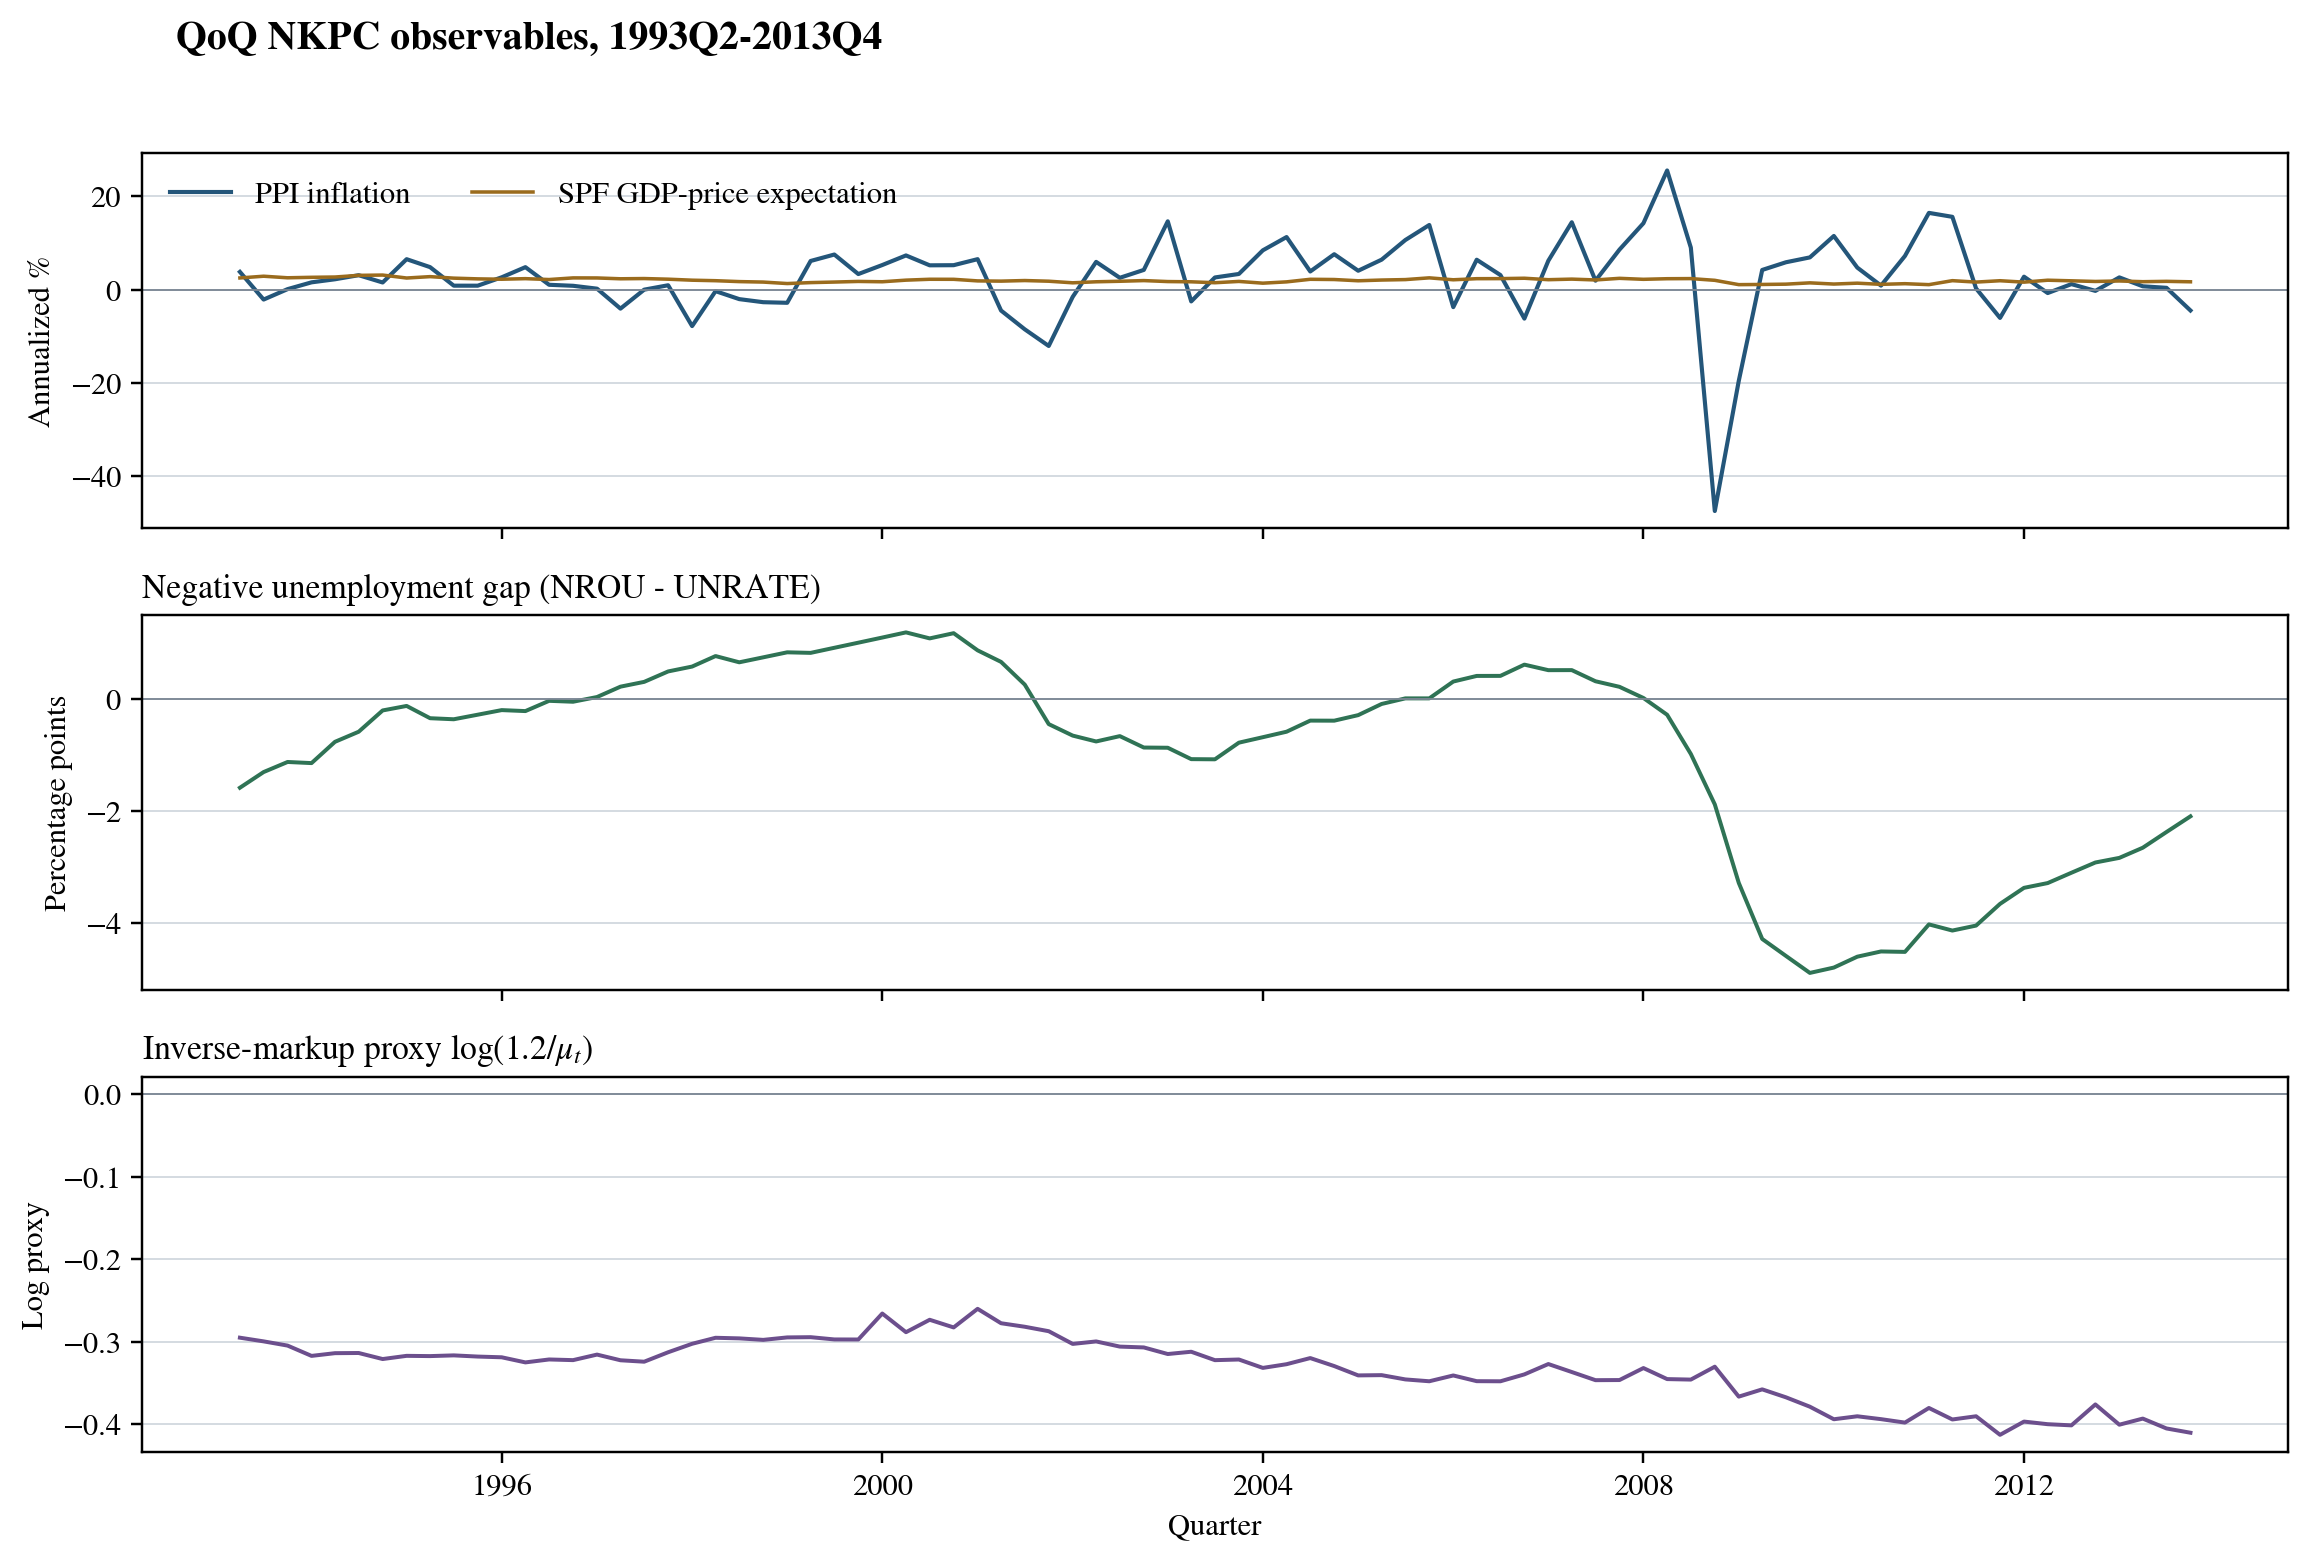
\includegraphics[width=0.92\linewidth]{data_timeseries.png}
\caption{Observed QoQ inflation, expectation, and activity series.}
\end{figure}

% -----------------------------------------------------------------------------
\section{Competition Inputs and Their Empirical Meaning}

\paragraph{Gustavo annual effective-firm count.}
The annual series is the inverse of the HHI of U.S. listed firms associated with
Grullon, Larkin, and Michaely. It supplies a long-run competition coordinate. The implemented
coordinate is
\begin{equation}
g_y=10\log(N_y^G/N_{1993}^G).
\end{equation}

\paragraph{Capital IQ quarterly effective-firm count.}
Capital IQ firm-quarter revenues for U.S. public firms on major exchanges are aggregated to
market HHIs and then to an economy-wide effective number of firms. The report uses both
firm-count-weighted and revenue-weighted market aggregation. The coordinate is
\begin{equation}
c_{j,t}=10\log(N_{j,t}^{CIQ}/N_{j,1993Q4}^{CIQ}).
\end{equation}

\paragraph{Why the levels are not equated.}
The two datasets have different firm universes, industry aggregation, and effective-count
scales. Consequently this report does not impose a common observed identity
$N_t=\Nbar_t+\Nhat_t$ across the two raw series. Instead, Gustavo determines the slow
coordinate, while Capital IQ determines a conditional quarterly cycle with an estimated
intercept, loading, and measurement error. The notation $\Nbar,\Nhat$ describes empirical
competition states; it is not yet a proof that the coordinate equals the theoretical HSA
mass of active firms.

\begin{figure}[H]
\centering
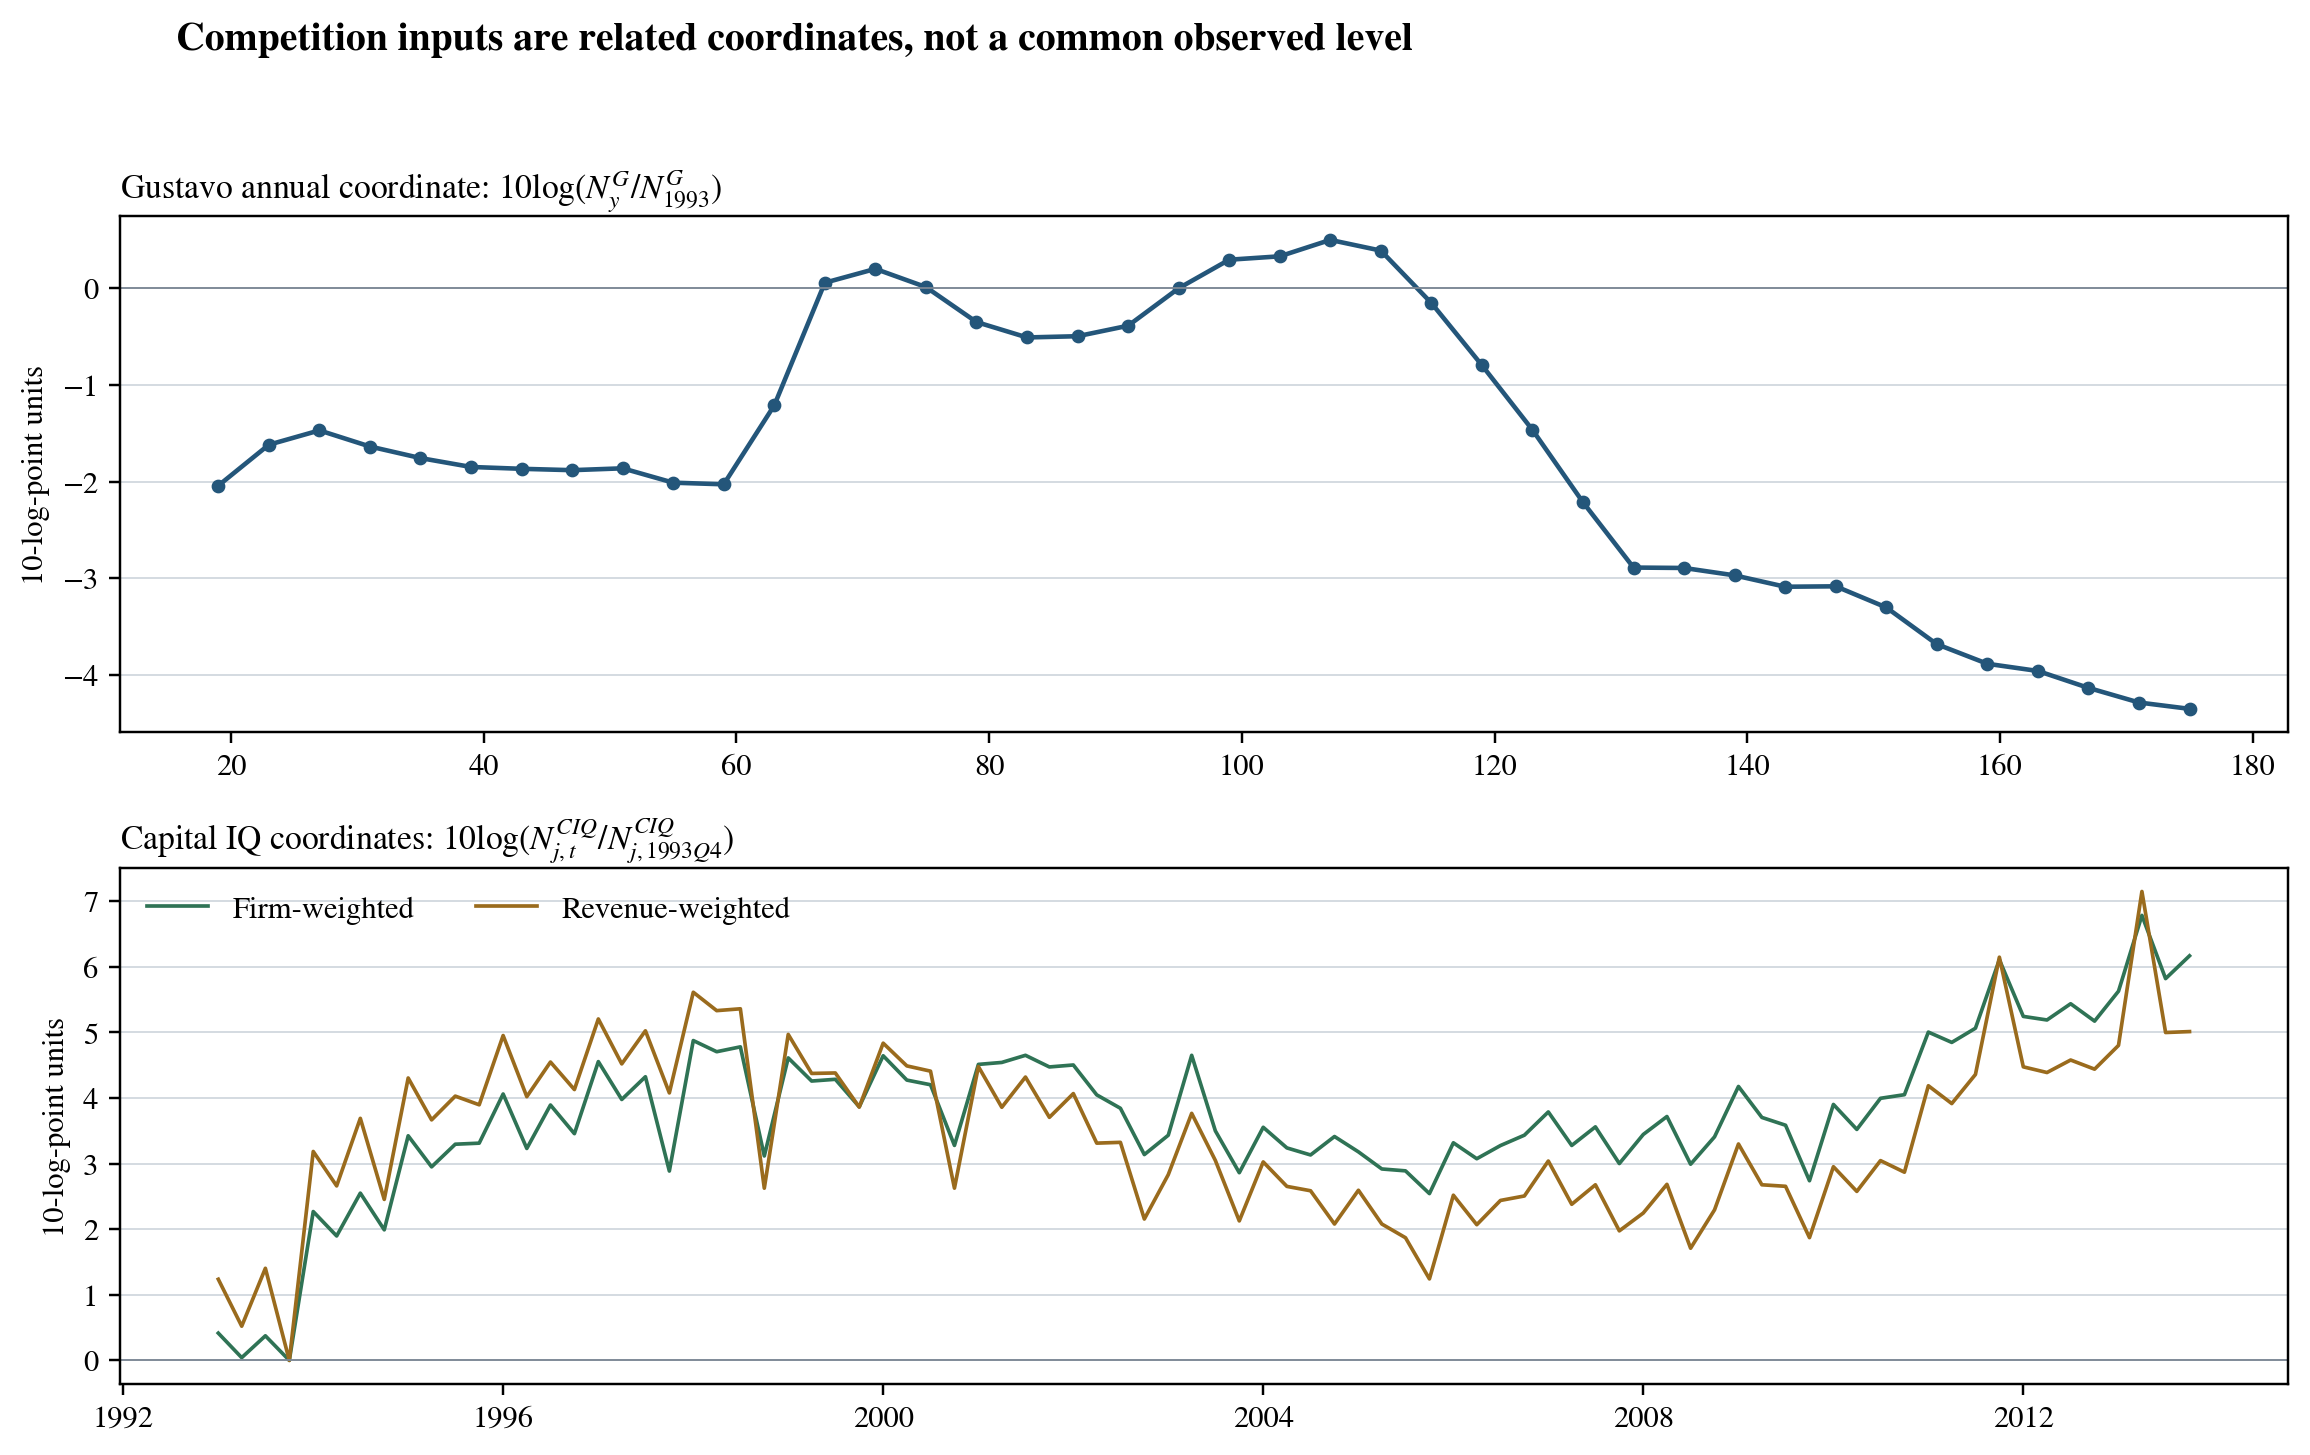
\includegraphics[width=0.88\linewidth]{competition_inputs.png}
\caption{Annual Gustavo and quarterly Capital IQ coordinates.}
\end{figure}

% -----------------------------------------------------------------------------
\section{Competition-State Measurement and the Modular Cut}

The annual Gustavo observations are exact Q4 endpoints of a quarterly Gaussian bridge,
\begin{align}
\Nbar_t&=\Nbar_{t-1}+\mu+\eta_t^{\bar n},\\
\Nbar_{y,Q4}&=g_y.
\end{align}
Conditional quarterly increments are drawn from the transition law subject to summing to
the observed annual change. This supplies a distribution over within-year timing without
deterministically interpolating the annual data.

Conditional on a slow-state draw, each Capital IQ coordinate satisfies
\begin{align}
c_{j,t}&=a_j+b_j\Nbar_t+\Nhat_{j,t}+e_{j,t},\\
\Nhat_{j,t}&=2r_j\cos(2\pi/P_j)\Nhat_{j,t-1}-r_j^2\Nhat_{j,t-2}+u_{j,t}.
\end{align}
The bounds $r_j\in[0.20,0.95]$ and $P_j\in[6,24]$ quarters keep the cycle stationary and
exclude an arbitrary second trend.

The ordering is
\begin{equation}
p(\Nbar\mid G)\;p(\Nhat,a,b,r,P,\sigma_h,\sigma_e\mid CIQ,\Nbar)\;
p(\text{NKPC coefficients}\mid\pi,x,E\pi,\Nbar,\Nhat).
\end{equation}
Inflation cannot update either competition state. This modular cut prevents the state-space
model from constructing a cycle merely because it helps explain inflation.

\begin{figure}[H]
\centering
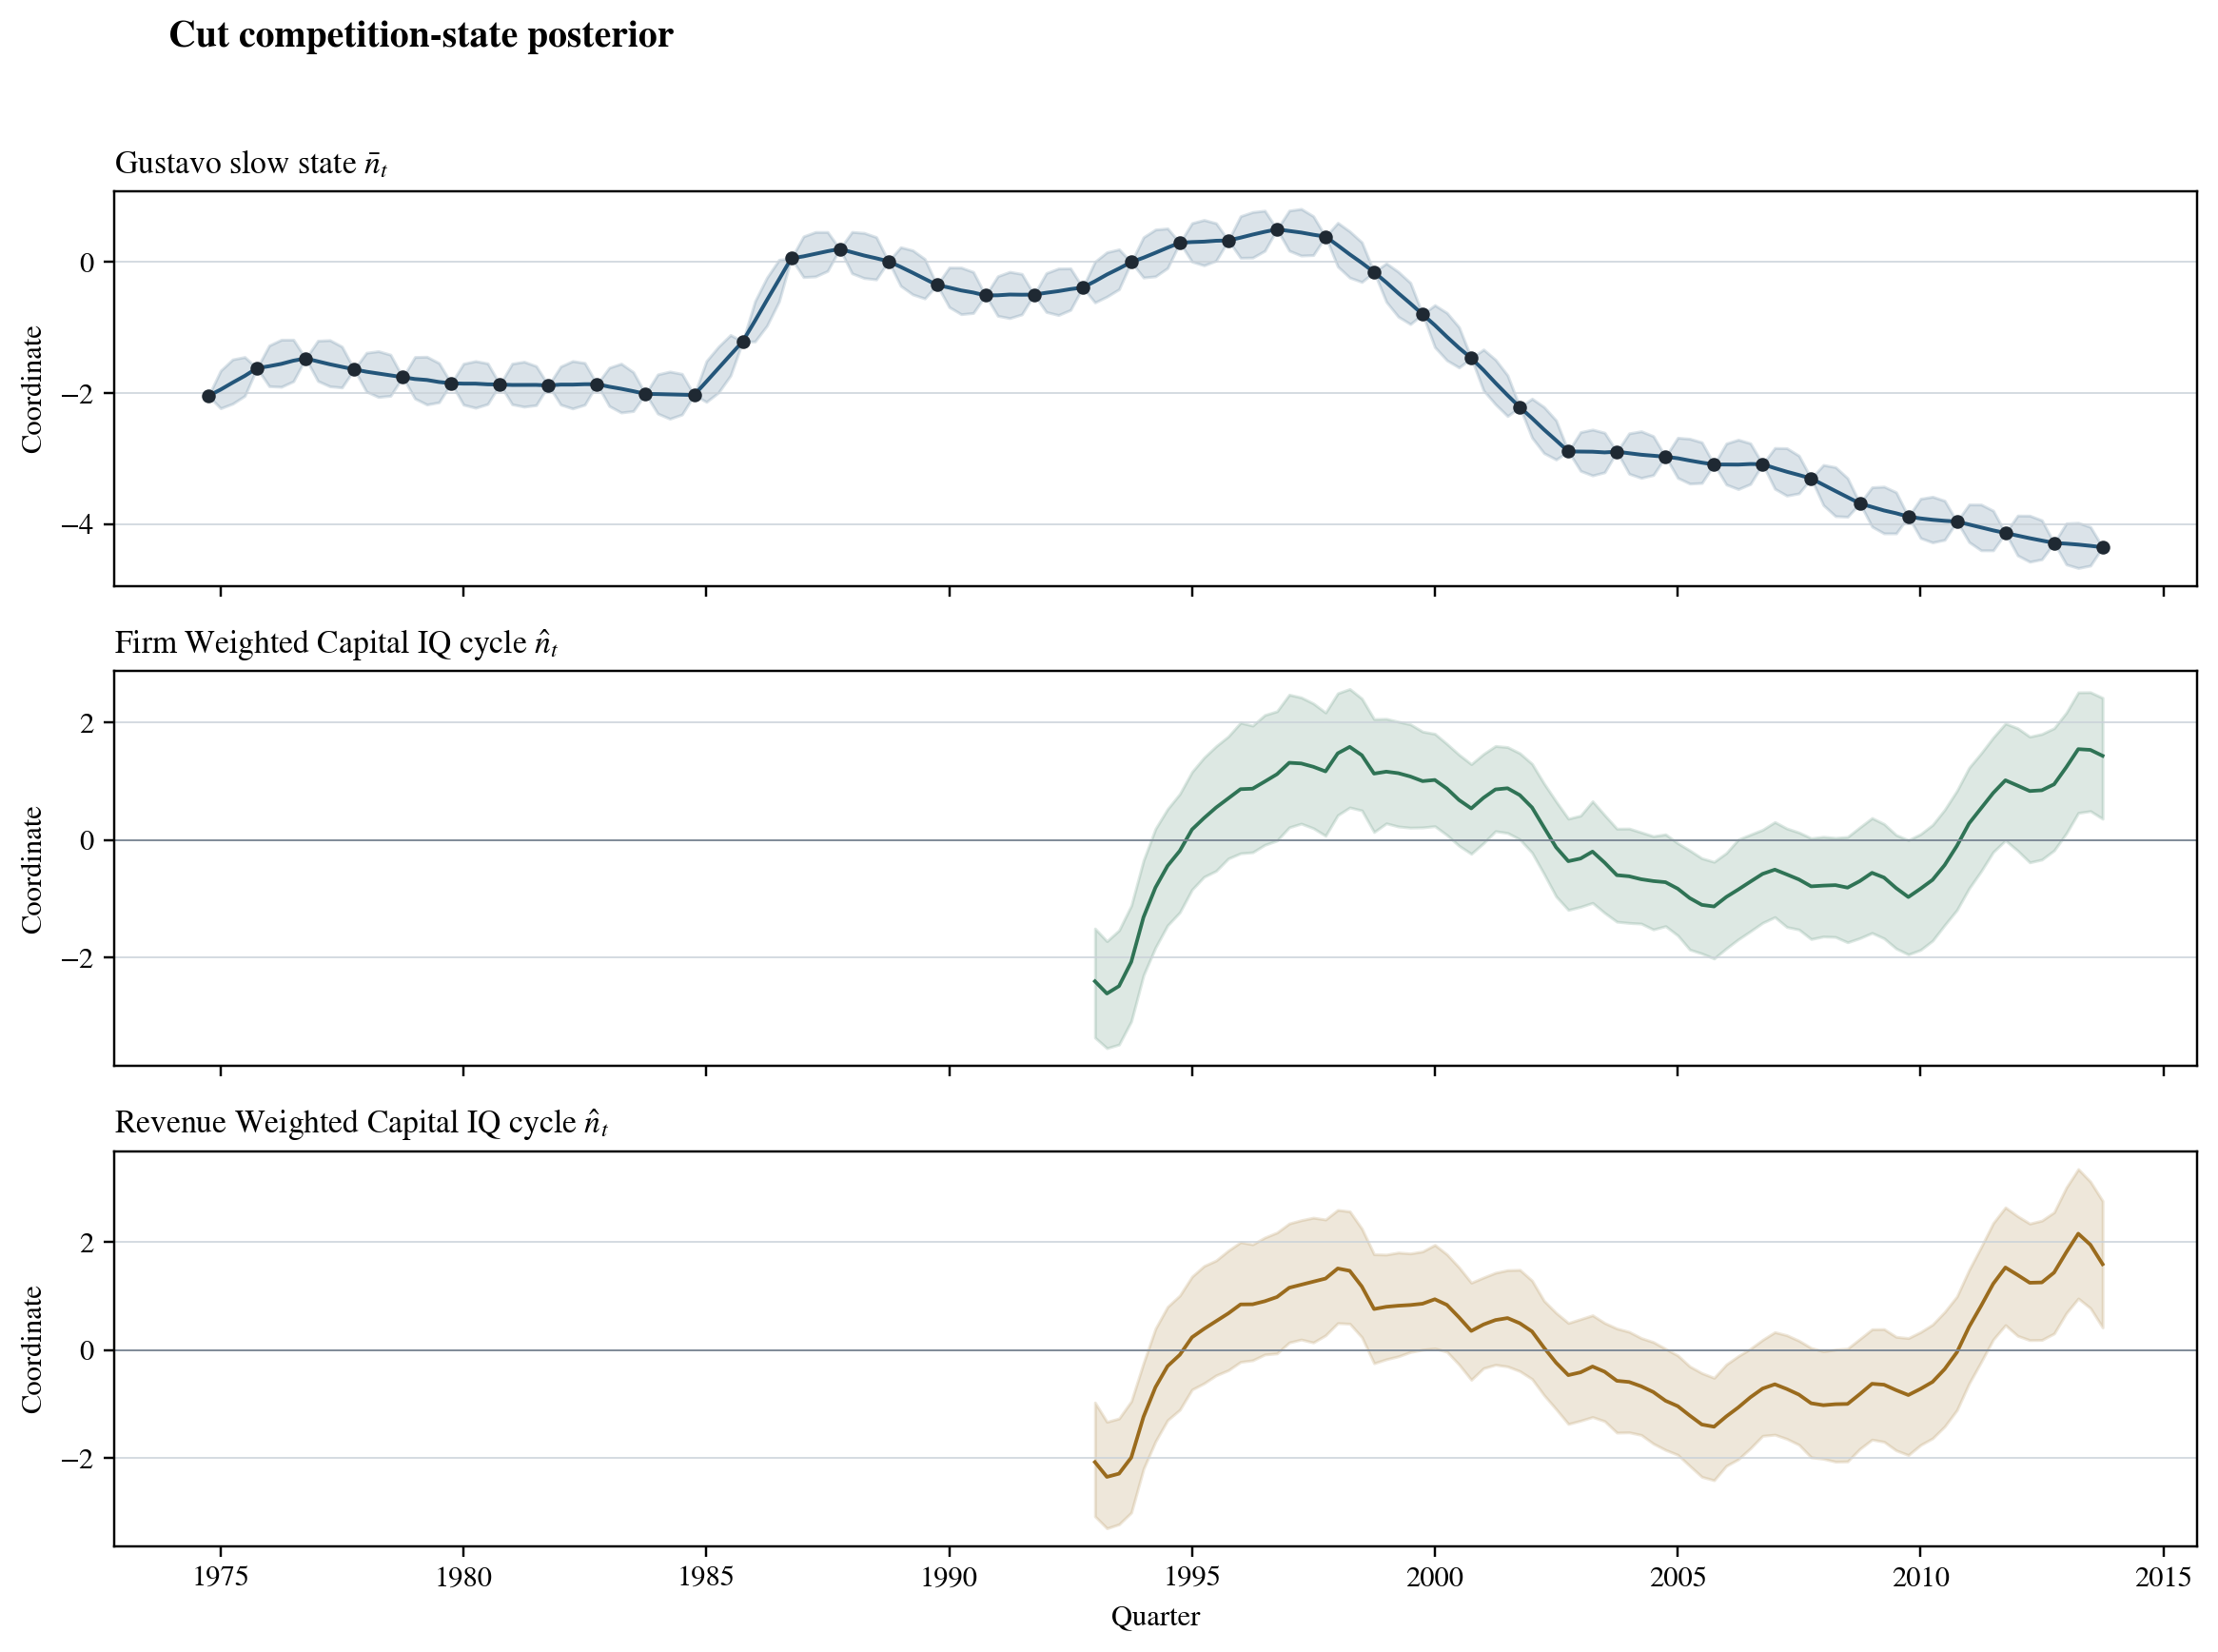
\includegraphics[width=0.92\linewidth]{state_decomposition.png}
\caption{Slow and cyclical competition-state posterior. Bands are pointwise 95\% intervals.}
\end{figure}

% -----------------------------------------------------------------------------
\section{Why the Models Are Estimated in This Order}

The estimation sequence is identification-first rather than restriction-first.

\begin{enumerate}
\item \textbf{Constant theta / direct only:} ask whether the quarterly Capital IQ cycle has
a free direct loading before using any slow-state slope information.
\item \textbf{Free static combined:} add a free slow slope $\delta$ and check whether
$\theta$ survives, without linking them.
\item \textbf{Recovery before restriction:} inject known $\delta$ and $\theta$ into the
actual 83-quarter design and test whether the unrestricted model can recover them.
\item \textbf{Varying theta:} add $\gamma$ without adding dynamic slope coefficients. This
isolates whether the direct loading itself varies.
\item \textbf{Free dynamic:} allow linear and quadratic slope variation independently.
\item \textbf{HSA-restricted dynamic:} only then impose the cross-equation restrictions and
compare their predictive implications.
\end{enumerate}

This ordering matters. If the free coefficients cannot be recovered, a product restriction
can create a narrower posterior by transferring information across equations. Such narrowing
is an implication of the restriction, not evidence that the direct channel was independently
identified.

The predeclared free-static gate failed and would ordinarily stop the dynamic branch. The
dynamic models in this report were estimated afterward at explicit user request as a weak-
identification diagnostic. They must be interpreted in that status.

% -----------------------------------------------------------------------------
\section{Estimated Model Hierarchy}

Let
\begin{equation}
\Nbar_t^c=\Nbar_t-T^{-1}\sum_s\Nbar_s,
\qquad
q_t^{(2)}=(\Nbar_t^c)^2-T^{-1}\sum_s(\Nbar_s^c)^2.
\end{equation}
Centering keeps $\kappa_0$ and $\theta_0$ at the sample-average slow state. Centering the
quadratic term changes only the intercept of $\kappa(\Nbar)$, not its derivative.

\subsection{M0: constant theta / direct only}
\begin{equation}
\kappa_t=\kappa_0,\qquad \theta_t=\theta.
\end{equation}
This is the minimum free-direct diagnostic.

\subsection{M1: free static combined}
\begin{equation}
\kappa_t=\kappa_0+\delta\Nbar_t^c,\qquad \theta_t=\theta.
\end{equation}
This asks whether the slow slope and cyclical direct channels coexist. It is not HSA-
restricted because $\delta$ and $\theta$ are independent.

\subsection{M2: varying theta}
\begin{equation}
\kappa_t=\kappa_0,\qquad \theta_t=\theta_0+\gamma\Nbar_t^c.
\end{equation}
This isolates time variation in the direct channel.

\subsection{M3: free dynamic}
\begin{equation}
\kappa_t=\kappa_0+\delta_1\Nbar_t^c+\delta_2q_t^{(2)},
\qquad \theta_t=\theta_0+\gamma\Nbar_t^c.
\end{equation}
It is the unrestricted benchmark for the HSA dynamic restriction.

\subsection{M4: HSA-restricted dynamic}
HSA links slope and direct channels through
\begin{equation}
\frac{d\kappa(N)}{dN}=\lambda\theta(N),\qquad \lambda=b_x\zeta.
\end{equation}
With $\theta(N)=\theta_0+\gamma N$, integration gives
\begin{equation}
\kappa_t=\kappa_0+\lambda\theta_0\Nbar_t^c
+\frac{\lambda\gamma}{2}q_t^{(2)},
\end{equation}
so the tested restrictions are
\begin{equation}
\boxed{\delta_1=\lambda\theta_0,\qquad
\delta_2=\lambda\gamma/2.}
\end{equation}
The sign of $\lambda$ is not fixed. Because Capital IQ is an empirical concentration
coordinate and $b_x$ is not externally identified here, $\lambda$ is a proportionality
parameter, not automatically a demand elasticity.

% -----------------------------------------------------------------------------
\section{Priors, Sampling, and Identification Criteria}

For every coefficient whose regressor is $z_t$, the competition prior is standardized so
one prior standard deviation contributes 0.20 inflation standard deviations:
\begin{equation}
\beta_z\sim N\!\left(0,
\left[0.20\frac{s_\pi}{s_z}\right]^2\right).
\end{equation}
The intercept prior is $N(0,(2s_\pi)^2)$,
$\alpha_b,\alpha_f\sim N(0.5,0.5^2)$, and
$\lambda\sim N(0,10^2)$. No economic sign is imposed. The innovation variance has the
common inverse-gamma update with shape 3 and scale $2s_\pi^2$. The AR(1) robustness prior is
$\rho\sim N(0,0.5^2)$ truncated to $[-0.95,0.95]$.

Constant-theta and free-static observed fits use four chains, 2,000 iterations, 600 warmup,
and thinning by two. The three dynamic specifications use four chains, 5,000 iterations,
1,500 warmup, and thinning by two. Observed dynamic fits require maximum R-hat at most 1.05
and minimum bulk ESS at least 400.

\paragraph{Learning versus sign evidence.}
Posterior narrowing is summarized by $SD_{post}/SD_{prior}$. Suggestive recovery requires a
correct-sign probability of at least 0.80 and an SD ratio at most 0.75. Strong recovery also
requires sign probability 0.975 and a 95\% interval excluding zero. Convergence, learning,
sign identification, and predictive performance are reported separately.

\begin{figure}[H]
\centering
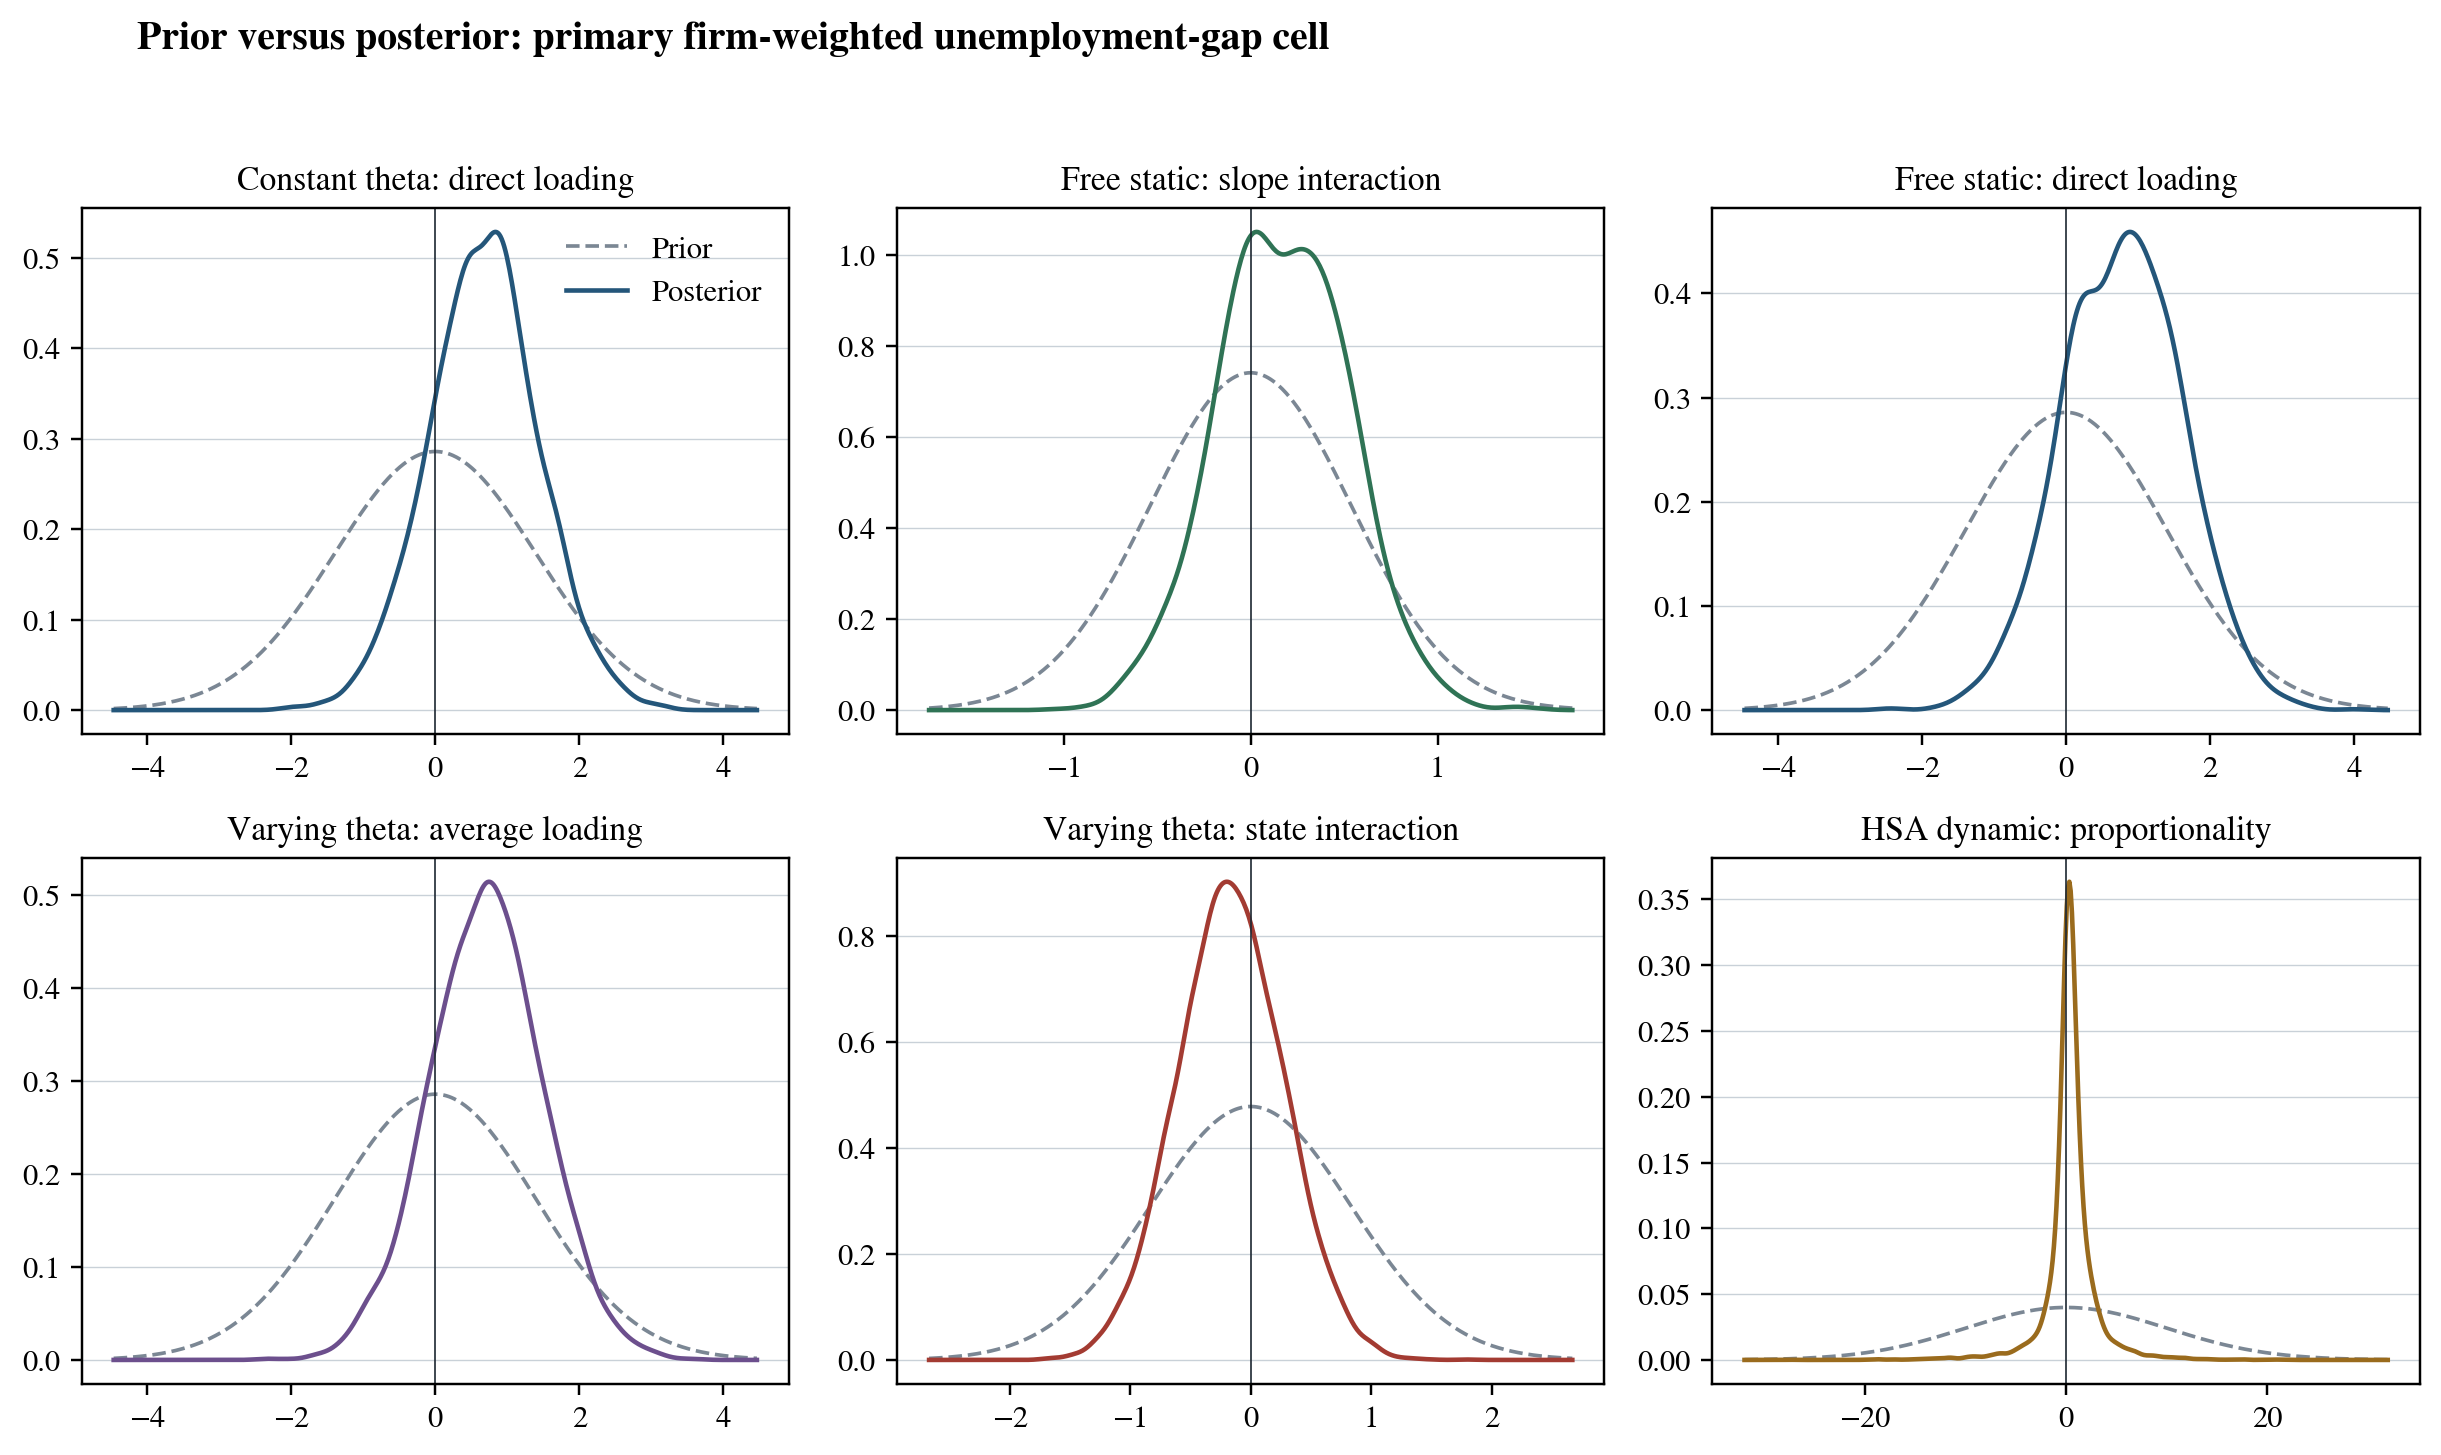
\includegraphics[width=0.92\linewidth]{prior_posterior_primary.png}
\caption{Selected prior-versus-posterior densities.}
\end{figure}

% -----------------------------------------------------------------------------
\section{Competition Measurement Results}

\begin{table}[H]
\centering
\caption{Competition-state parameters; posterior mean and 95\% interval}
\scriptsize
\begin{tabular}{@{}lllc@{}}
\toprule
Block & Variant & Parameter & Posterior \\
\midrule
gustavo\_slow & gustavo & mu & \makecell{-0.015\\{\scriptsize [-0.045, 0.015]}} \\
gustavo\_slow & gustavo & sigma\_bar & \makecell{0.179\\{\scriptsize [0.146, 0.222]}} \\
capital\_iq\_cycle & firm\_weighted & intercept & \makecell{2.860\\{\scriptsize [2.038, 3.704]}} \\
capital\_iq\_cycle & firm\_weighted & loading & \makecell{-0.383\\{\scriptsize [-0.761, -0.061]}} \\
capital\_iq\_cycle & firm\_weighted & damping & \makecell{0.779\\{\scriptsize [0.617, 0.892]}} \\
capital\_iq\_cycle & firm\_weighted & period & \makecell{20.204\\{\scriptsize [15.715, 23.735]}} \\
capital\_iq\_cycle & firm\_weighted & sigma\_cycle & \makecell{0.310\\{\scriptsize [0.181, 0.538]}} \\
capital\_iq\_cycle & firm\_weighted & sigma\_measurement & \makecell{0.462\\{\scriptsize [0.352, 0.576]}} \\
capital\_iq\_cycle & revenue\_weighted & intercept & \makecell{3.442\\{\scriptsize [2.541, 4.122]}} \\
capital\_iq\_cycle & revenue\_weighted & loading & \makecell{0.027\\{\scriptsize [-0.295, 0.330]}} \\
capital\_iq\_cycle & revenue\_weighted & damping & \makecell{0.756\\{\scriptsize [0.600, 0.879]}} \\
capital\_iq\_cycle & revenue\_weighted & period & \makecell{19.436\\{\scriptsize [14.752, 23.643]}} \\
capital\_iq\_cycle & revenue\_weighted & sigma\_cycle & \makecell{0.363\\{\scriptsize [0.212, 0.568]}} \\
capital\_iq\_cycle & revenue\_weighted & sigma\_measurement & \makecell{0.660\\{\scriptsize [0.528, 0.814]}} \\
\bottomrule
\end{tabular}

\end{table}

The exact Gustavo Q4 anchor error is below $10^{-15}$. The slow innovation scale is
$0.179[0.146,0.222]$ in the ten-log-point coordinate. Capital IQ cycles are persistent but
stationary: damping is about 0.76--0.78 and the posterior periods are about 19--20 quarters.

The most consequential measurement result is the slow loading. Firm weighting gives
$b=-0.383[-0.761,-0.061]$, whereas revenue weighting gives
$0.027[-0.295,0.330]$. The two datasets therefore do not support a stable one-for-one level
mapping. The negative firm loading is not interpreted as a structural negative relation;
it may reflect listed-firm coverage, entry/exit composition, market weighting, or industry
aggregation differences. This is precisely why the report gives the two datasets distinct
measurement roles.

The cycle measurement error is also material: $\sigma_e$ is 0.462 for firm weighting and
0.660 for revenue weighting. Propagating this uncertainty is empirically important; treating
the posterior median cycle as known would overstate precision.

% -----------------------------------------------------------------------------
\section{M0 Results: Constant Direct Loading}

The estimated equation is displayed again next to its results:
\begin{equation}
\pi_t^q=a+\alpha_b\pi_{t-1}^q+\alpha_fE_t\pi_{t+1}^q
+\kappa_0x_t-\theta_{CIQ}\Nhat_t+\varepsilon_t.
\end{equation}

\begin{table}[H]
\centering
\caption{Constant-theta model; posterior mean and 95\% interval}
\resizebox{\linewidth}{!}{\begin{tabular}{@{}lcccc@{}}
\toprule
Parameter & Firm / unemployment & Revenue / unemployment & Firm / inverse markup & Revenue / inverse markup \\
\midrule
alpha\_b & \makecell{0.342\\{\scriptsize [0.139, 0.545]}} & \makecell{0.344\\{\scriptsize [0.139, 0.548]}} & \makecell{0.339\\{\scriptsize [0.131, 0.545]}} & \makecell{0.336\\{\scriptsize [0.134, 0.547]}} \\
alpha\_f & \makecell{0.393\\{\scriptsize [-0.566, 1.328]}} & \makecell{0.407\\{\scriptsize [-0.527, 1.368]}} & \makecell{0.412\\{\scriptsize [-0.540, 1.356]}} & \makecell{0.406\\{\scriptsize [-0.528, 1.326]}} \\
kappa\_0 & \makecell{-0.019\\{\scriptsize [-0.943, 0.897]}} & \makecell{-0.077\\{\scriptsize [-0.986, 0.793]}} & \makecell{-11.227\\{\scriptsize [-48.249, 28.316]}} & \makecell{-12.844\\{\scriptsize [-51.463, 25.927]}} \\
theta\_CIQ & \makecell{0.674\\{\scriptsize [-0.845, 2.200]}} & \makecell{0.609\\{\scriptsize [-0.783, 2.055]}} & \makecell{0.656\\{\scriptsize [-0.843, 2.176]}} & \makecell{0.669\\{\scriptsize [-0.762, 2.065]}} \\
\bottomrule
\end{tabular}
}
\end{table}

The direct coefficient is positive on average in all four cells. Posterior positive
probabilities are approximately 0.79--0.84, and posterior SD is about 54--57\% of prior SD.
This is genuine updating from a symmetric zero-mean prior. It is not, however, strong sign
identification: every 95\% interval includes zero.

The backward inflation coefficient is well learned near 0.34. In contrast, the forward
coefficient remains close to its $N(0.5,0.5^2)$ prior in dispersion. This is another source
of uncertainty: the expectation term can absorb low-frequency variation that might otherwise
help estimate the competition loadings.

The inverse-markup $\kappa_0$ is numerically large because the inverse-markup proxy has a
sample SD of only 0.038. It must not be compared directly with the unemployment-gap slope.

% -----------------------------------------------------------------------------
\section{M1 Results: Free Static Combined Channels}

The free-static equation is
\begin{equation}
\pi_t^q=a+\alpha_b\pi_{t-1}^q+\alpha_fE_t\pi_{t+1}^q
+(\kappa_0+\delta\Nbar_t^c)x_t-\theta_{CIQ}\Nhat_t+\varepsilon_t.
\end{equation}

\begin{table}[H]
\centering
\caption{Free-static combined model; posterior mean and 95\% interval}
\resizebox{\linewidth}{!}{\begin{tabular}{@{}lcccc@{}}
\toprule
Parameter & Firm / unemployment & Revenue / unemployment & Firm / inverse markup & Revenue / inverse markup \\
\midrule
kappa\_0 & \makecell{0.198\\{\scriptsize [-1.055, 1.475]}} & \makecell{0.081\\{\scriptsize [-1.110, 1.290]}} & \makecell{-9.952\\{\scriptsize [-52.861, 36.946]}} & \makecell{-11.476\\{\scriptsize [-56.517, 29.453]}} \\
delta & \makecell{0.173\\{\scriptsize [-0.517, 0.861]}} & \makecell{0.141\\{\scriptsize [-0.567, 0.874]}} & \makecell{0.221\\{\scriptsize [-2.779, 3.255]}} & \makecell{0.214\\{\scriptsize [-2.813, 3.173]}} \\
theta\_CIQ & \makecell{0.784\\{\scriptsize [-0.832, 2.388]}} & \makecell{0.710\\{\scriptsize [-0.802, 2.198]}} & \makecell{0.672\\{\scriptsize [-0.874, 2.189]}} & \makecell{0.630\\{\scriptsize [-0.851, 2.063]}} \\
\bottomrule
\end{tabular}
}
\end{table}

Adding the slow slope interaction does not eliminate the direct update. In the two primary
IID unemployment-gap cells, $P(\theta_{CIQ}>0)$ is about 0.83. The largest absolute posterior
correlation between $\delta$ and $\theta_{CIQ}$ is 0.352, below the predeclared severe-
confounding threshold of 0.80.

But every $\delta$ interval includes zero. The fixed 2010Q1--2013Q4 holdout ELPD is lower
for free static in all four cells, and the Savage--Dickey $BF_{01}$ lies between 1.38 and
1.57, mildly favoring $\delta=0$. Thus the slow slope term does not explain away theta, but
neither does it earn empirical support of its own.

\begin{figure}[H]
\centering
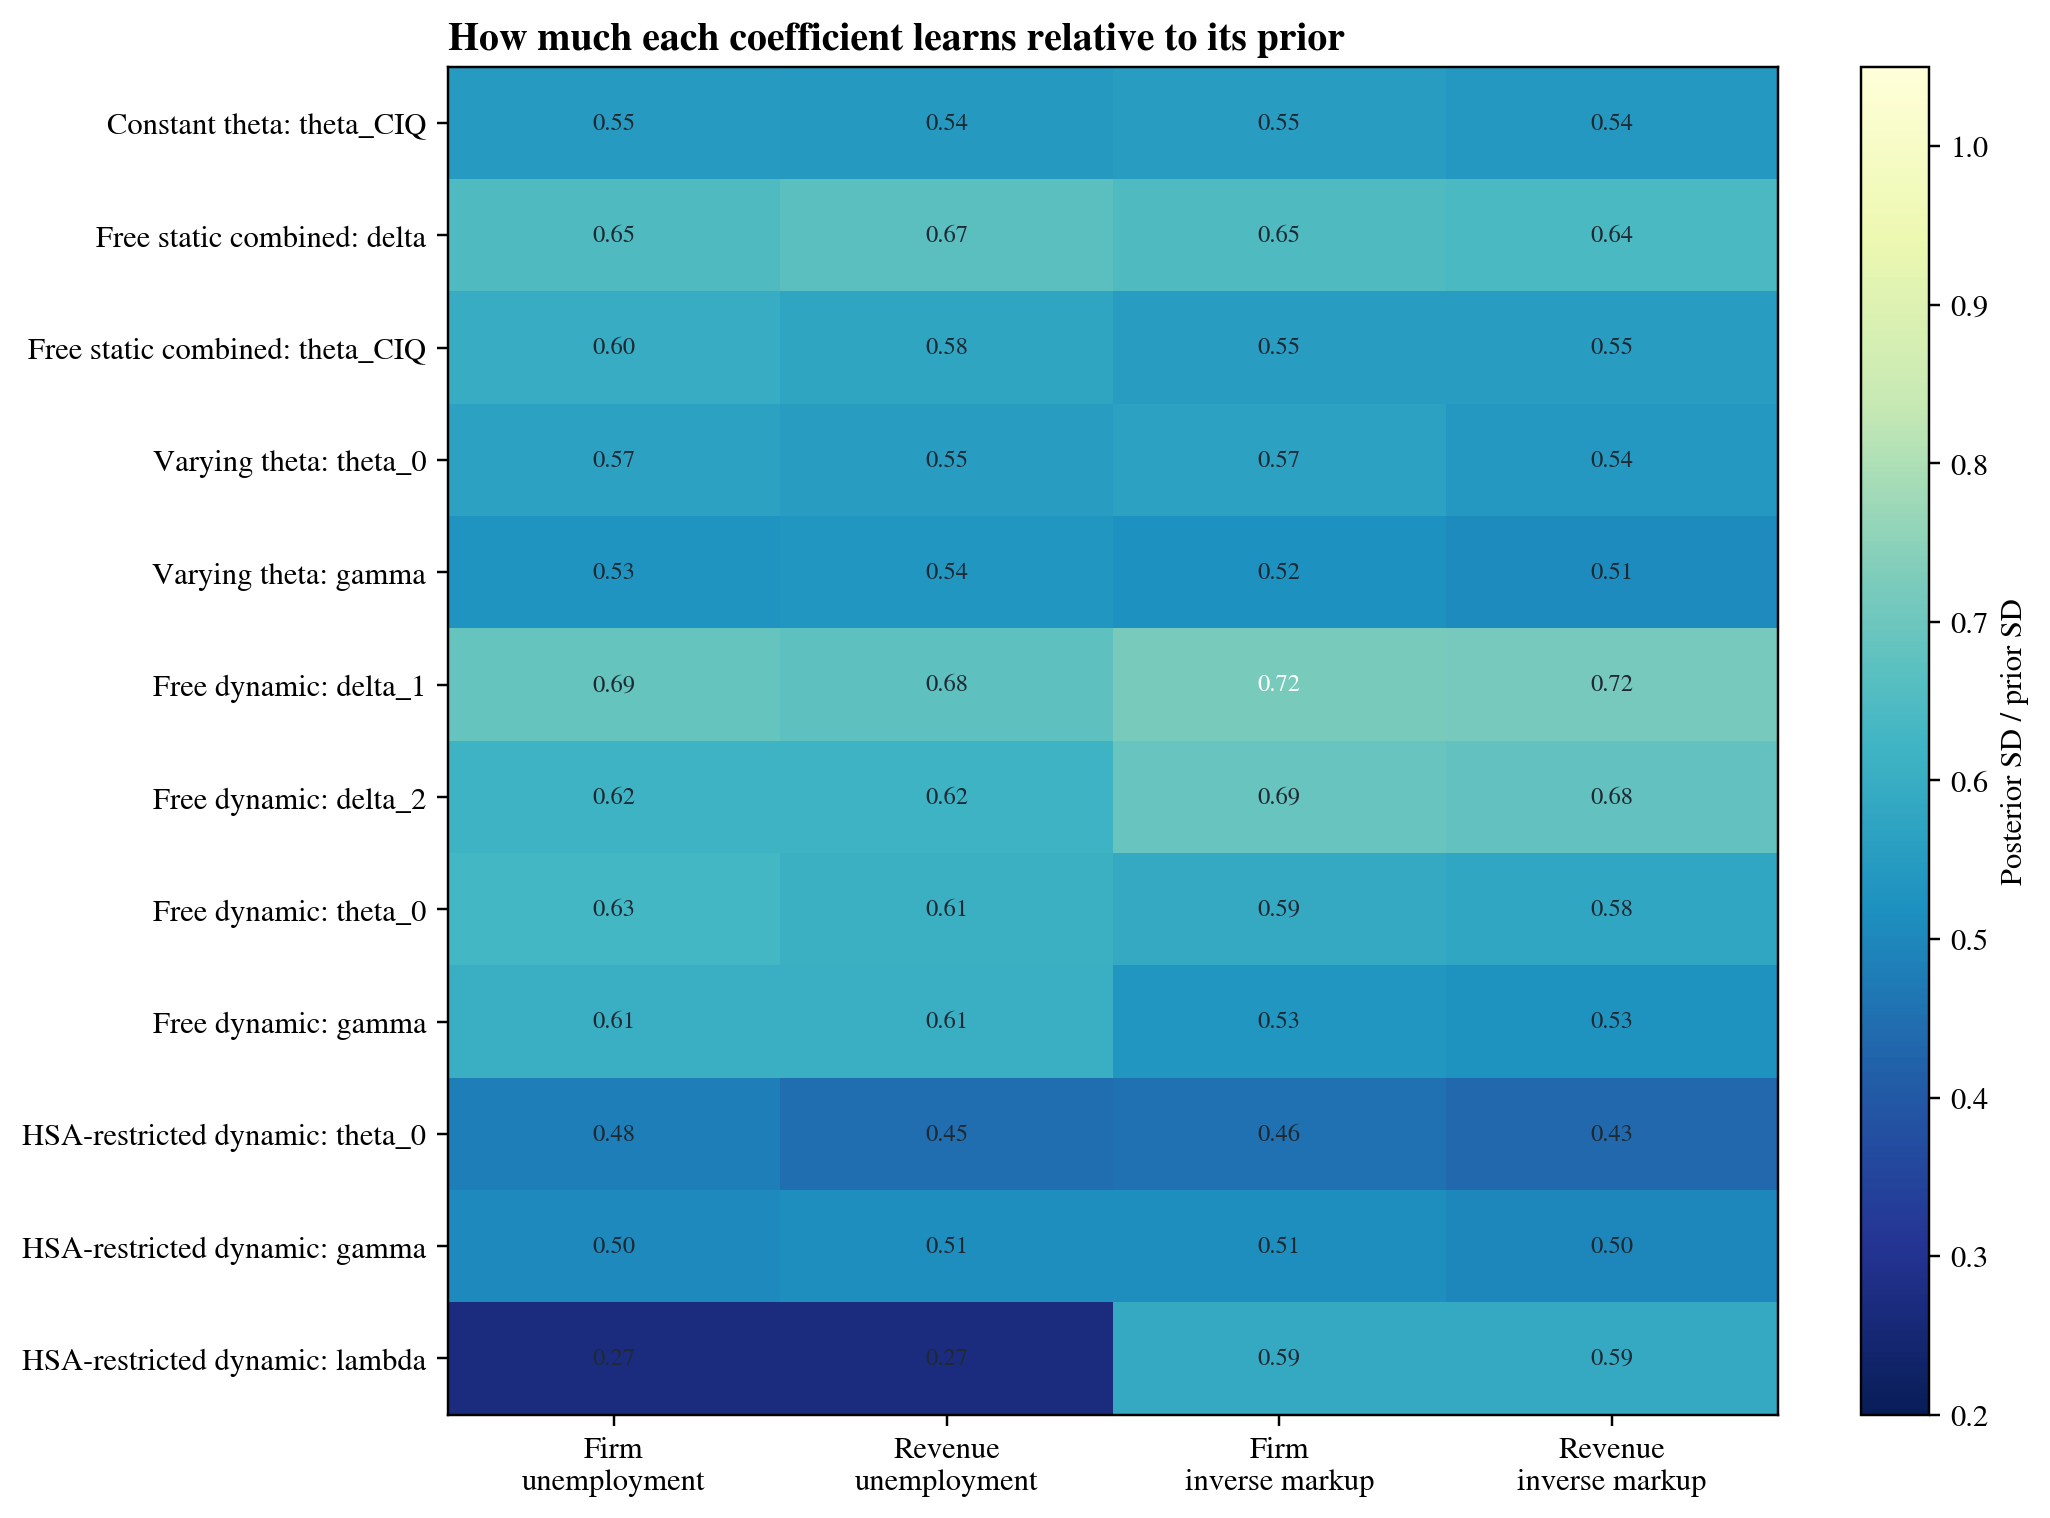
\includegraphics[width=0.89\linewidth]{learning_heatmap.png}
\caption{Posterior-to-prior SD ratios for target competition coefficients. Lower values mean more learning, not necessarily correct-sign identification.}
\end{figure}

% -----------------------------------------------------------------------------
\section{Simulation Recovery Before Imposing HSA}

Static recovery simulates the actual sample, activity series, inflation persistence, and
paired competition states, injecting standardized effects
\begin{equation}
s_\theta=\theta\,SD(\Nhat)/SD(\pi),\qquad
s_\delta=\delta\,SD(\Nbar^c x)/SD(\pi).
\end{equation}
The observed unemployment-gap magnitudes are approximately
$(s_\delta,s_\theta)=(0.06,0.11)$.

\begin{table}[H]
\centering
\caption{Primary propagated-state free-static recovery}
\input{tables/recovery_static.tex}
\end{table}

At observed magnitudes, suggestive recovery is 0.10 for $\delta$ and 0.333 for theta,
against the predeclared 0.80 promotion threshold. Oracle-state recovery is only 0.133 and
0.333. State measurement uncertainty is therefore not the main bottleneck; the aggregate
design and effect sizes are.

The recovery computation itself passes: maximum R-hat is 1.0395, minimum bulk ESS is 100.6,
coverage is 1.00 at the observed scenario, and null false-positive rates are zero. The gate
fails because detection is weak, not because the simulation sampler failed.

\begin{figure}[H]
\centering
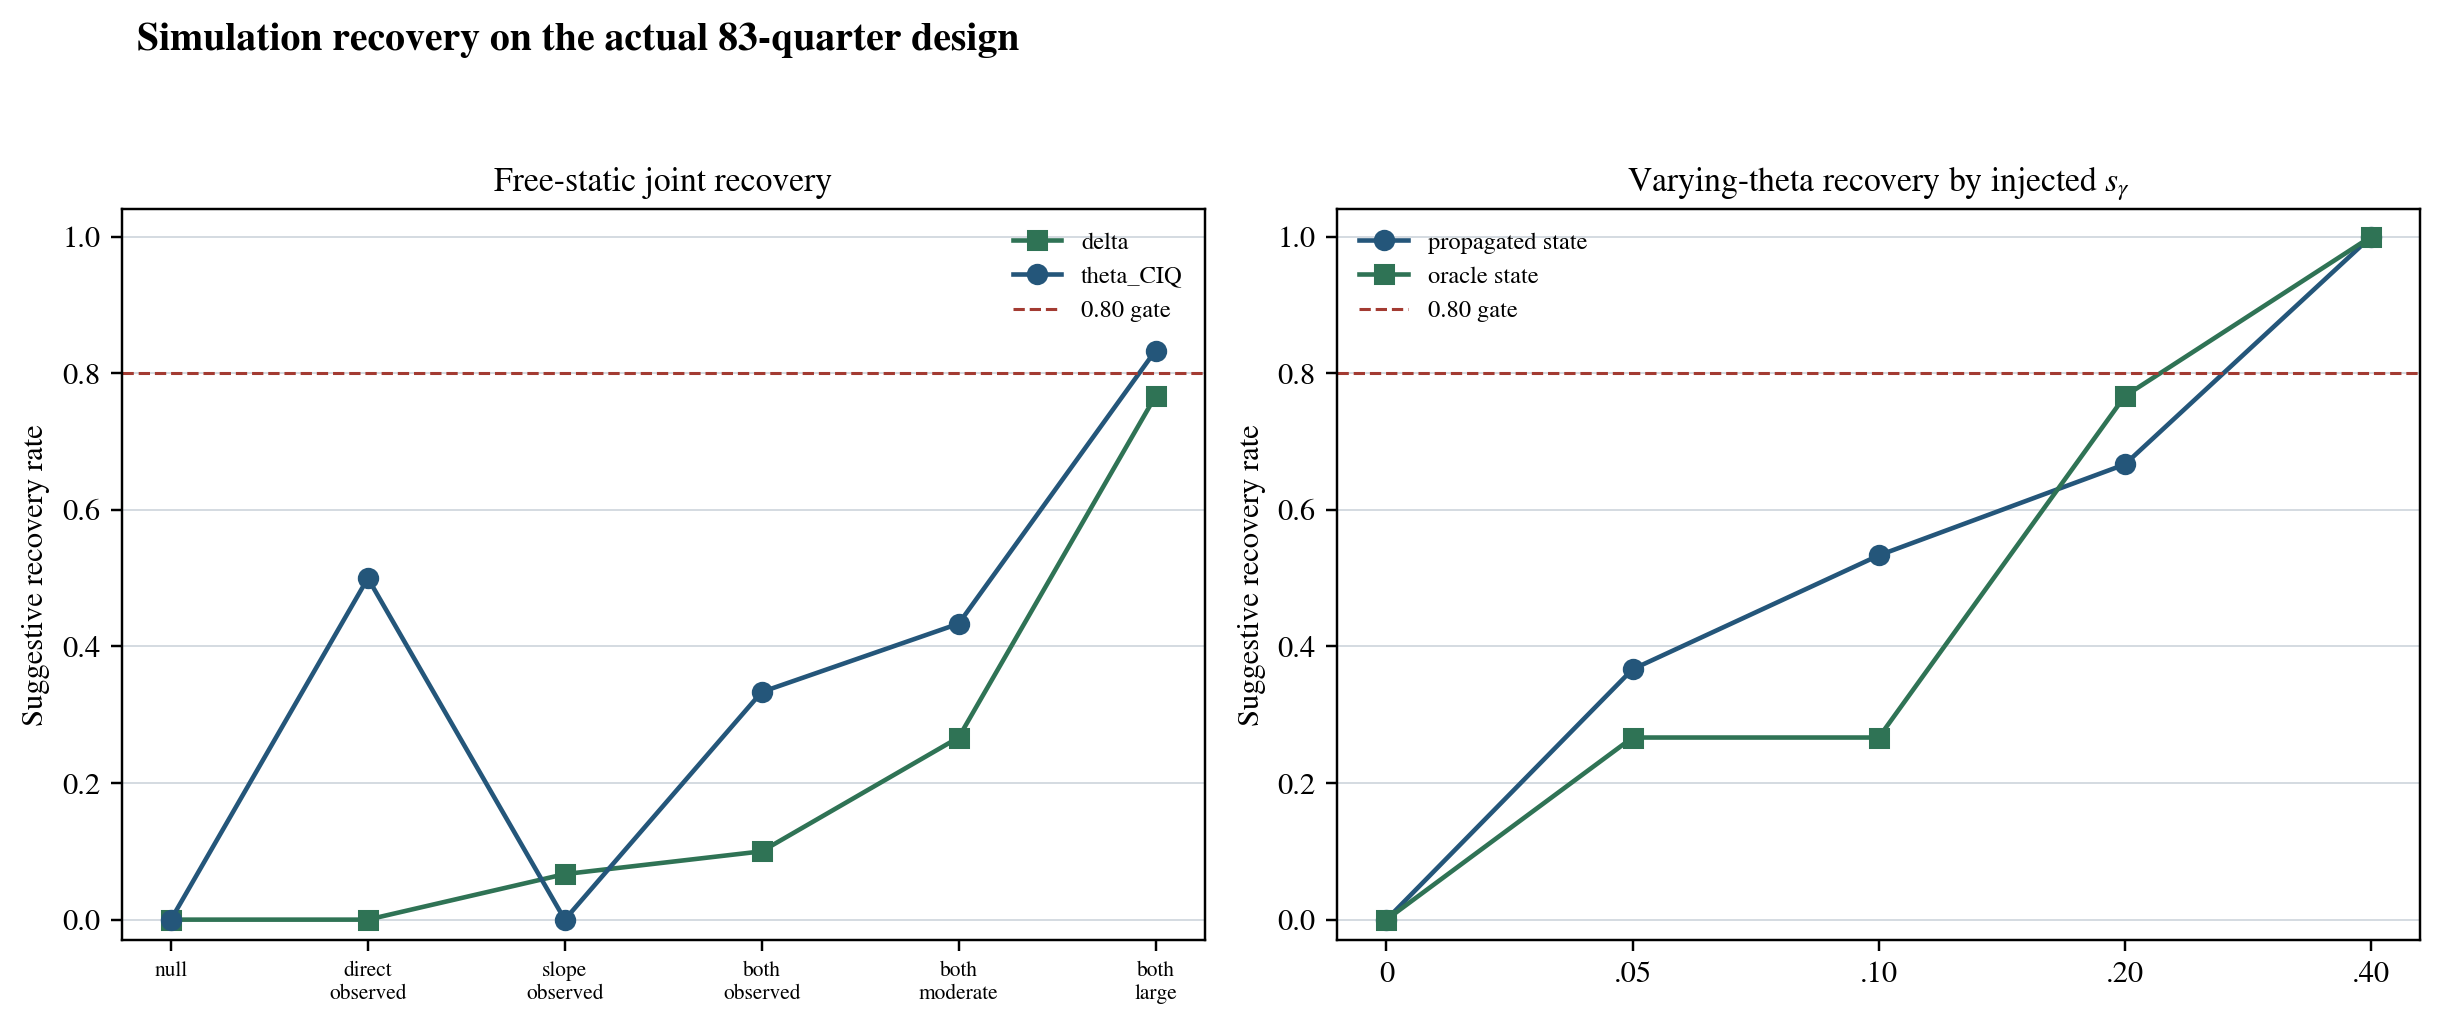
\includegraphics[width=0.94\linewidth]{recovery.png}
\caption{Free-static and varying-theta recovery on the actual sample design.}
\end{figure}

% -----------------------------------------------------------------------------
\section{M2 Results: Is Theta Time-Varying?}

The isolated varying-theta equation is
\begin{equation}
\pi_t^q=a+\alpha_b\pi_{t-1}^q+\alpha_fE_t\pi_{t+1}^q
+\kappa_0x_t-(\theta_0+\gamma\Nbar_t^c)\Nhat_t+\varepsilon_t.
\end{equation}

\begin{table}[H]
\centering
\caption{Varying-theta model; posterior mean and 95\% interval}
\resizebox{\linewidth}{!}{\begin{tabular}{@{}lcccc@{}}
\toprule
Parameter & Firm / unemployment & Revenue / unemployment & Firm / inverse markup & Revenue / inverse markup \\
\midrule
kappa\_0 & \makecell{-0.061\\{\scriptsize [-1.035, 0.920]}} & \makecell{-0.119\\{\scriptsize [-1.112, 0.848]}} & \makecell{-13.378\\{\scriptsize [-53.205, 26.472]}} & \makecell{-14.644\\{\scriptsize [-55.328, 24.334]}} \\
theta\_0 & \makecell{0.710\\{\scriptsize [-0.865, 2.262]}} & \makecell{0.627\\{\scriptsize [-0.830, 2.077]}} & \makecell{0.749\\{\scriptsize [-0.813, 2.283]}} & \makecell{0.666\\{\scriptsize [-0.754, 2.099]}} \\
gamma & \makecell{-0.165\\{\scriptsize [-1.030, 0.707]}} & \makecell{-0.126\\{\scriptsize [-0.953, 0.701]}} & \makecell{-0.215\\{\scriptsize [-1.083, 0.645]}} & \makecell{-0.170\\{\scriptsize [-0.960, 0.610]}} \\
\bottomrule
\end{tabular}
}
\end{table}

$\theta_0$ remains directionally positive: $P(\theta_0>0)$ ranges from 0.804 to 0.830.
Every interval still includes zero. More importantly, every $\gamma$ posterior leans
negative and includes zero; $P(\gamma>0)$ ranges from 0.308 to 0.384. The data therefore do
not reveal positive time variation in the direct channel.

The varying-theta recovery fixes $s_{\theta_0}=0.11$ and injects
$s_\gamma\in\{0,0.05,0.10,0.20,0.40\}$. Thirty propagated-state and thirty oracle-state
replications are used at each value.

\begin{table}[H]
\centering
\caption{Propagated-state recovery of $\gamma$}
\begin{tabular}{@{}rrrrr@{}}
\toprule
True $s_\gamma$ & Suggestive & Strong & Coverage & Mean SD ratio \\
\midrule
0.00 & 0.000 & 0.000 & 1.000 & 0.522 \\
0.05 & 0.367 & 0.000 & 1.000 & 0.523 \\
0.10 & 0.533 & 0.067 & 1.000 & 0.521 \\
0.20 & 0.667 & 0.167 & 1.000 & 0.510 \\
0.40 & 1.000 & 0.800 & 0.967 & 0.520 \\
\bottomrule
\end{tabular}

\end{table}

At $s_\gamma=0.10$, suggestive recovery is 0.533 but strong recovery is only 0.067. Strong
recovery reaches 0.80 only at $s_\gamma=0.40$. Modest time variation is below the practical
detection threshold of this aggregate sample.

% -----------------------------------------------------------------------------
\section{M3 Results: Free Dynamic Channels}

The unrestricted dynamic benchmark is
\begin{align}
\theta_t&=\theta_0+\gamma\Nbar_t^c,\\
\kappa_t&=\kappa_0+\delta_1\Nbar_t^c+\delta_2q_t^{(2)}.
\end{align}

\begin{table}[H]
\centering
\caption{Free-dynamic model; posterior mean and 95\% interval}
\resizebox{\linewidth}{!}{\begin{tabular}{@{}lcccc@{}}
\toprule
Parameter & Firm / unemployment & Revenue / unemployment & Firm / inverse markup & Revenue / inverse markup \\
\midrule
kappa\_0 & \makecell{0.118\\{\scriptsize [-1.215, 1.451]}} & \makecell{0.050\\{\scriptsize [-1.245, 1.309]}} & \makecell{-16.294\\{\scriptsize [-64.777, 31.296]}} & \makecell{-18.518\\{\scriptsize [-66.930, 31.734]}} \\
delta\_1 & \makecell{0.102\\{\scriptsize [-0.615, 0.851]}} & \makecell{0.115\\{\scriptsize [-0.595, 0.838]}} & \makecell{-0.076\\{\scriptsize [-3.463, 3.262]}} & \makecell{-0.130\\{\scriptsize [-3.383, 3.238]}} \\
delta\_2 & \makecell{-0.177\\{\scriptsize [-1.156, 0.803]}} & \makecell{-0.138\\{\scriptsize [-1.134, 0.830]}} & \makecell{0.813\\{\scriptsize [-1.530, 3.137]}} & \makecell{0.828\\{\scriptsize [-1.516, 3.191]}} \\
theta\_0 & \makecell{0.894\\{\scriptsize [-0.845, 2.598]}} & \makecell{0.750\\{\scriptsize [-0.857, 2.327]}} & \makecell{0.613\\{\scriptsize [-0.993, 2.296]}} & \makecell{0.518\\{\scriptsize [-0.988, 2.040]}} \\
gamma & \makecell{-0.241\\{\scriptsize [-1.257, 0.746]}} & \makecell{-0.171\\{\scriptsize [-1.104, 0.766]}} & \makecell{-0.191\\{\scriptsize [-1.064, 0.693]}} & \makecell{-0.157\\{\scriptsize [-0.957, 0.663]}} \\
\bottomrule
\end{tabular}
}
\end{table}

All sixteen target intervals for $\delta_1,\delta_2,\theta_0,\gamma$ include zero.
$\theta_0$ keeps a positive direction, with $P(\theta_0>0)$ from 0.750 to 0.847, but
$\gamma$ remains negative-leaning. Neither the linear nor quadratic slope change is
independently identified.

This model is essential even though it is weak. It shows what the data say before HSA links
the channels. Any precision gain in the restricted model must be assessed against these
wide free coefficients.

% -----------------------------------------------------------------------------
\section{M4 Results: HSA-Restricted Dynamic Model}

The fully restricted equation is
\begin{align}
\pi_t^q={}&a+\alpha_b\pi_{t-1}^q+\alpha_fE_t\pi_{t+1}^q\\
&+\left(\kappa_0+\lambda\theta_0\Nbar_t^c
+\frac{\lambda\gamma}{2}q_t^{(2)}\right)x_t\\
&-(\theta_0+\gamma\Nbar_t^c)\Nhat_t+\varepsilon_t.
\end{align}

\begin{table}[H]
\centering
\caption{HSA-restricted dynamic model; posterior mean and 95\% interval}
\resizebox{0.94\linewidth}{!}{\begin{tabular}{@{}lcccc@{}}
\toprule
Parameter & Firm / unemployment & Revenue / unemployment & Firm / inverse markup & Revenue / inverse markup \\
\midrule
kappa\_0 & \makecell{0.106\\{\scriptsize [-1.247, 1.526]}} & \makecell{0.051\\{\scriptsize [-1.250, 1.426]}} & \makecell{-14.523\\{\scriptsize [-65.287, 33.928]}} & \makecell{-15.291\\{\scriptsize [-66.327, 32.481]}} \\
theta\_0 & \makecell{0.406\\{\scriptsize [-0.619, 2.035]}} & \makecell{0.334\\{\scriptsize [-0.620, 1.837]}} & \makecell{0.375\\{\scriptsize [-0.664, 1.832]}} & \makecell{0.332\\{\scriptsize [-0.653, 1.678]}} \\
gamma & \makecell{-0.090\\{\scriptsize [-0.949, 0.721]}} & \makecell{-0.084\\{\scriptsize [-0.927, 0.719]}} & \makecell{-0.175\\{\scriptsize [-0.996, 0.668]}} & \makecell{-0.170\\{\scriptsize [-0.922, 0.639]}} \\
lambda & \makecell{0.402\\{\scriptsize [-5.288, 5.952]}} & \makecell{0.523\\{\scriptsize [-5.307, 6.244]}} & \makecell{-0.411\\{\scriptsize [-13.298, 12.196]}} & \makecell{-0.518\\{\scriptsize [-12.947, 12.155]}} \\
derived:delta\_1 & \makecell{0.149\\{\scriptsize [-0.644, 1.033]}} & \makecell{0.132\\{\scriptsize [-0.648, 1.013]}} & \makecell{-0.028\\{\scriptsize [-3.901, 3.895]}} & \makecell{0.022\\{\scriptsize [-3.796, 3.808]}} \\
derived:delta\_2 & \makecell{-0.016\\{\scriptsize [-0.705, 0.615]}} & \makecell{-0.010\\{\scriptsize [-0.691, 0.651]}} & \makecell{0.427\\{\scriptsize [-1.181, 3.065]}} & \makecell{0.396\\{\scriptsize [-1.204, 2.957]}} \\
\bottomrule
\end{tabular}
}
\end{table}

Every $\lambda$ interval spans zero and both signs:
\begin{equation*}
\lambda_{\mathrm{firm,unemp}}=0.402[-5.288,5.952],\qquad
\lambda_{\mathrm{firm,markup}}=-0.411[-13.298,12.196].
\end{equation*}
Every derived $\delta_1=\lambda\theta_0$ and
$\delta_2=\lambda\gamma/2$ interval also spans zero.

The narrower $\theta_0$ posterior in the restricted parameterization is not independent
direct-channel identification. The likelihood observes products such as
$\lambda\theta_0$ and $\lambda\gamma$. When the unrestricted factors are near zero, many
combinations of signs and magnitudes generate similar fitted values. This produces a weakly
identified multiplicative geometry. The restriction shares information; it does not create
new variation in the data.

% -----------------------------------------------------------------------------
\section{Implied Time-Varying Coefficients and In-Sample Fit}

\begin{figure}[H]
\centering
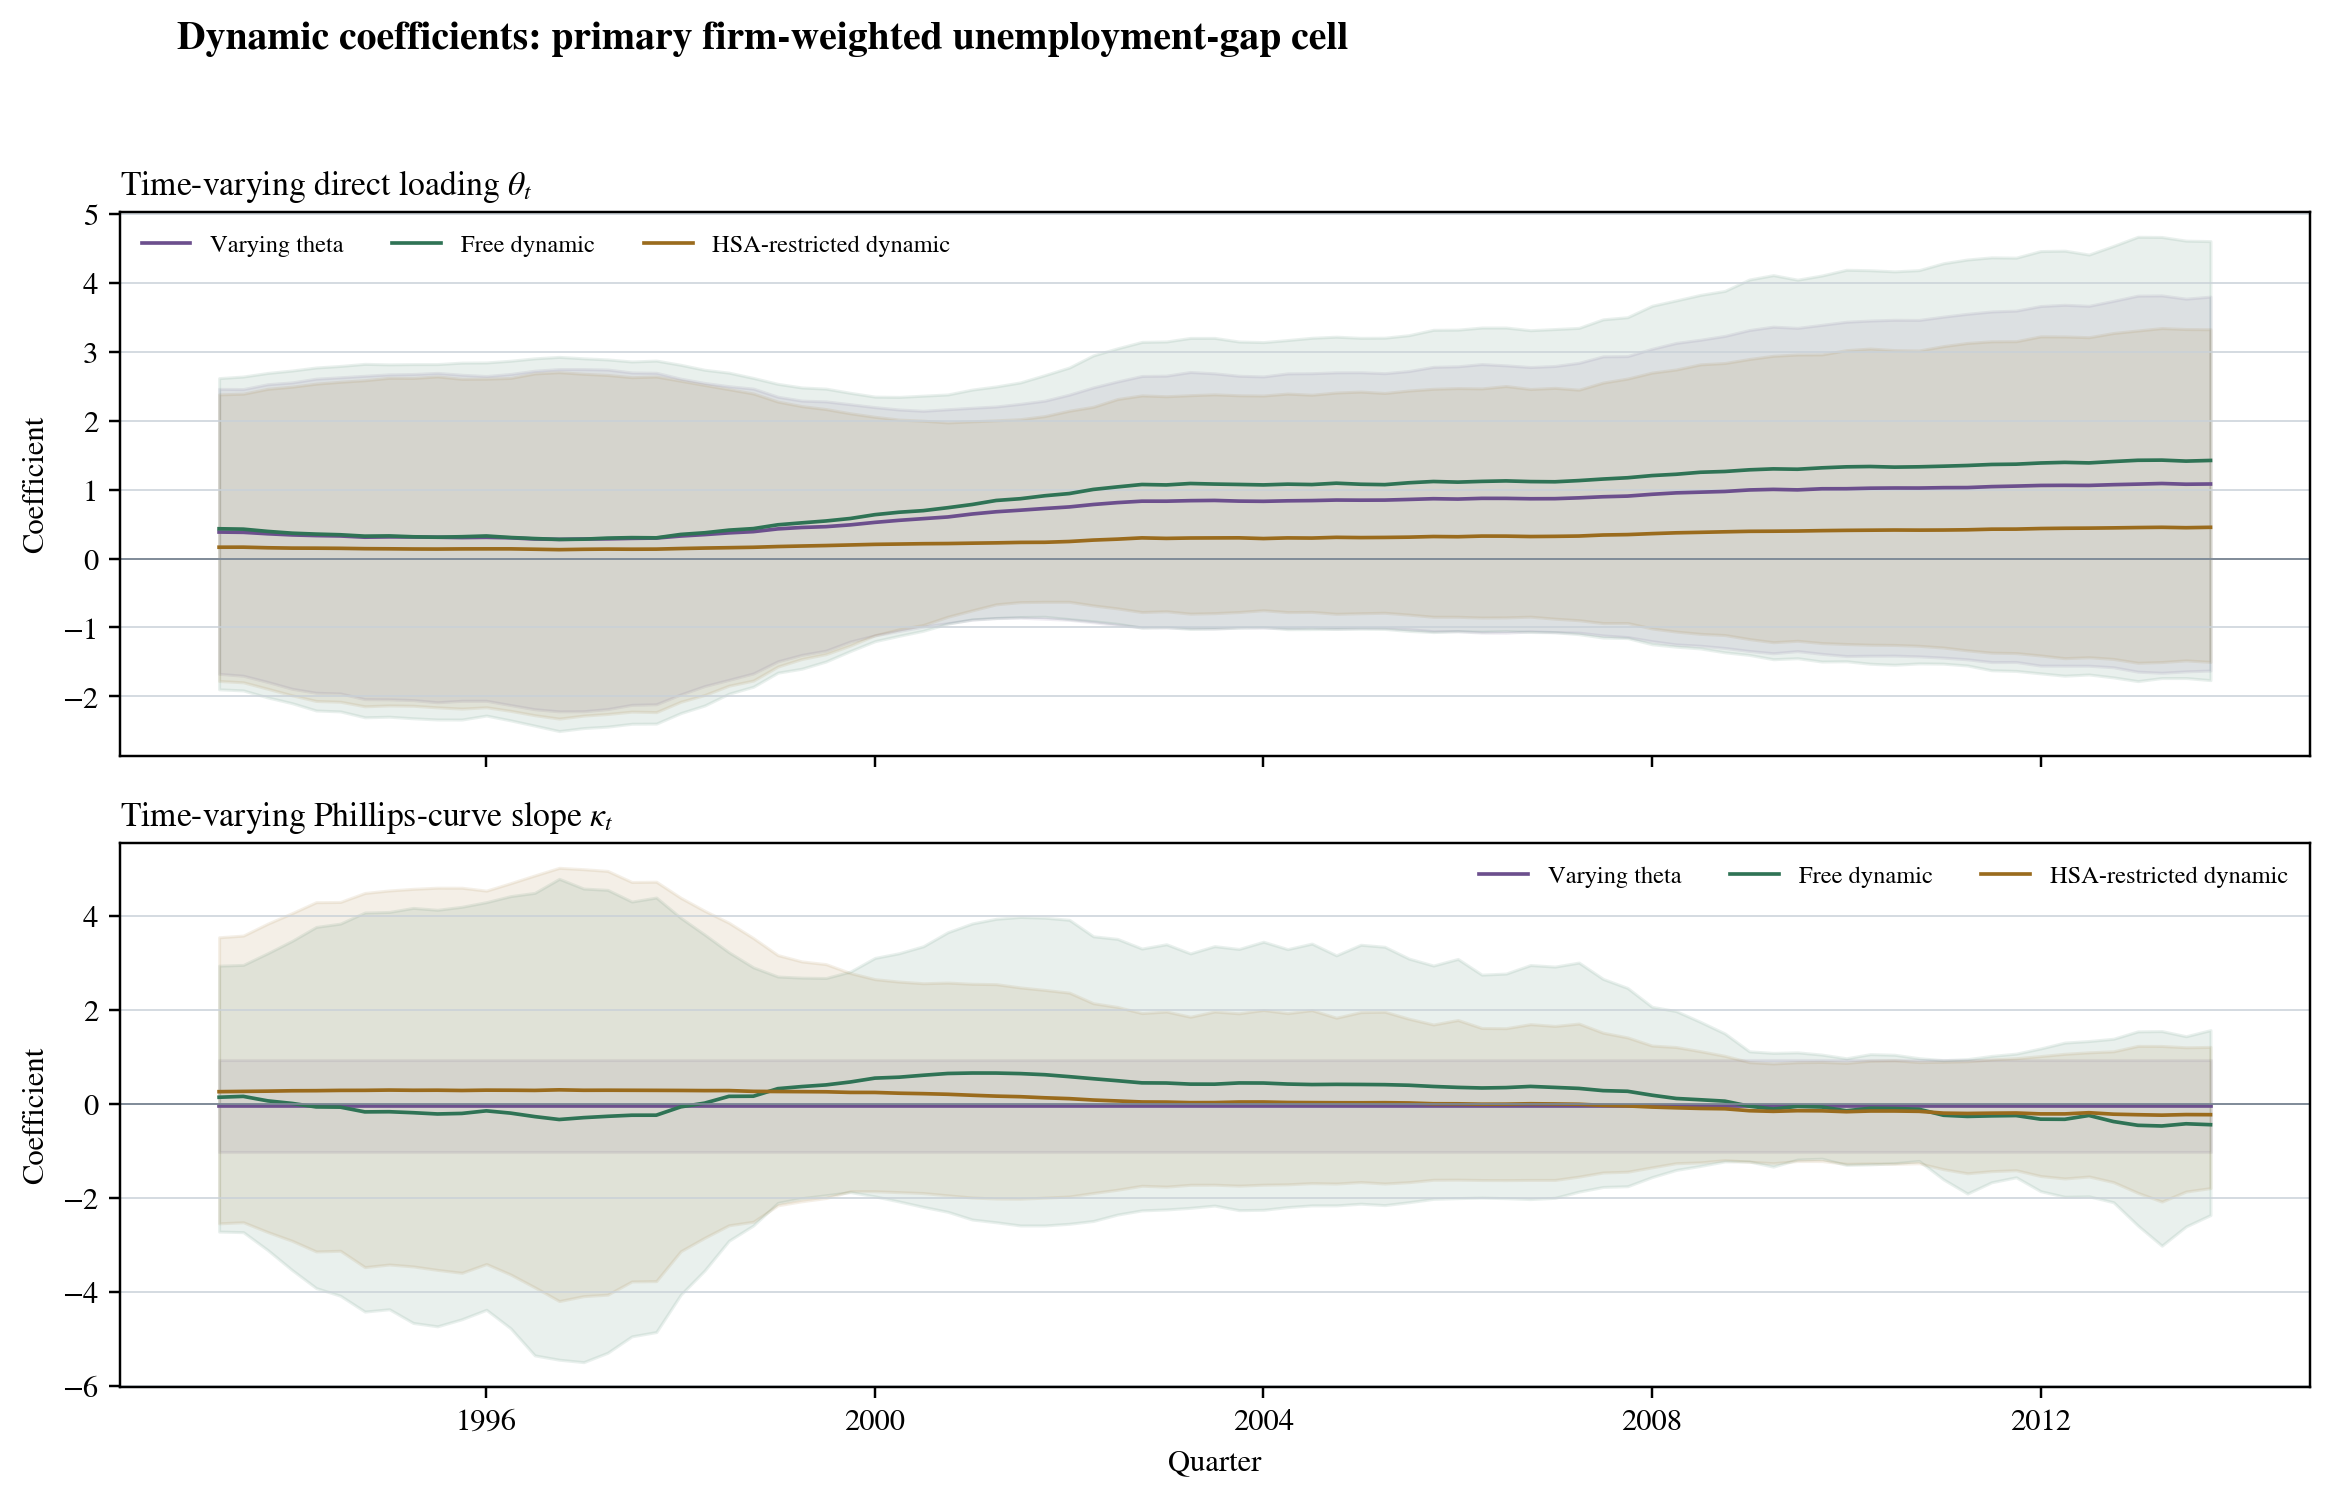
\includegraphics[width=0.94\linewidth]{dynamic_paths.png}
\caption{Posterior paths for the firm-weighted negative-unemployment-gap cell. Bands are pointwise 95\% intervals.}
\end{figure}

The posterior medians move because they are functions of the estimated slow-state path.
That visual movement must not be read as evidence that $\gamma$ or the quadratic slope is
identified. The bands remain wide and generally overlap zero. In particular, a smooth median
path can be mechanically induced by multiplying an uncertain coefficient by a smooth
$\Nbar_t$.

\begin{figure}[H]
\centering
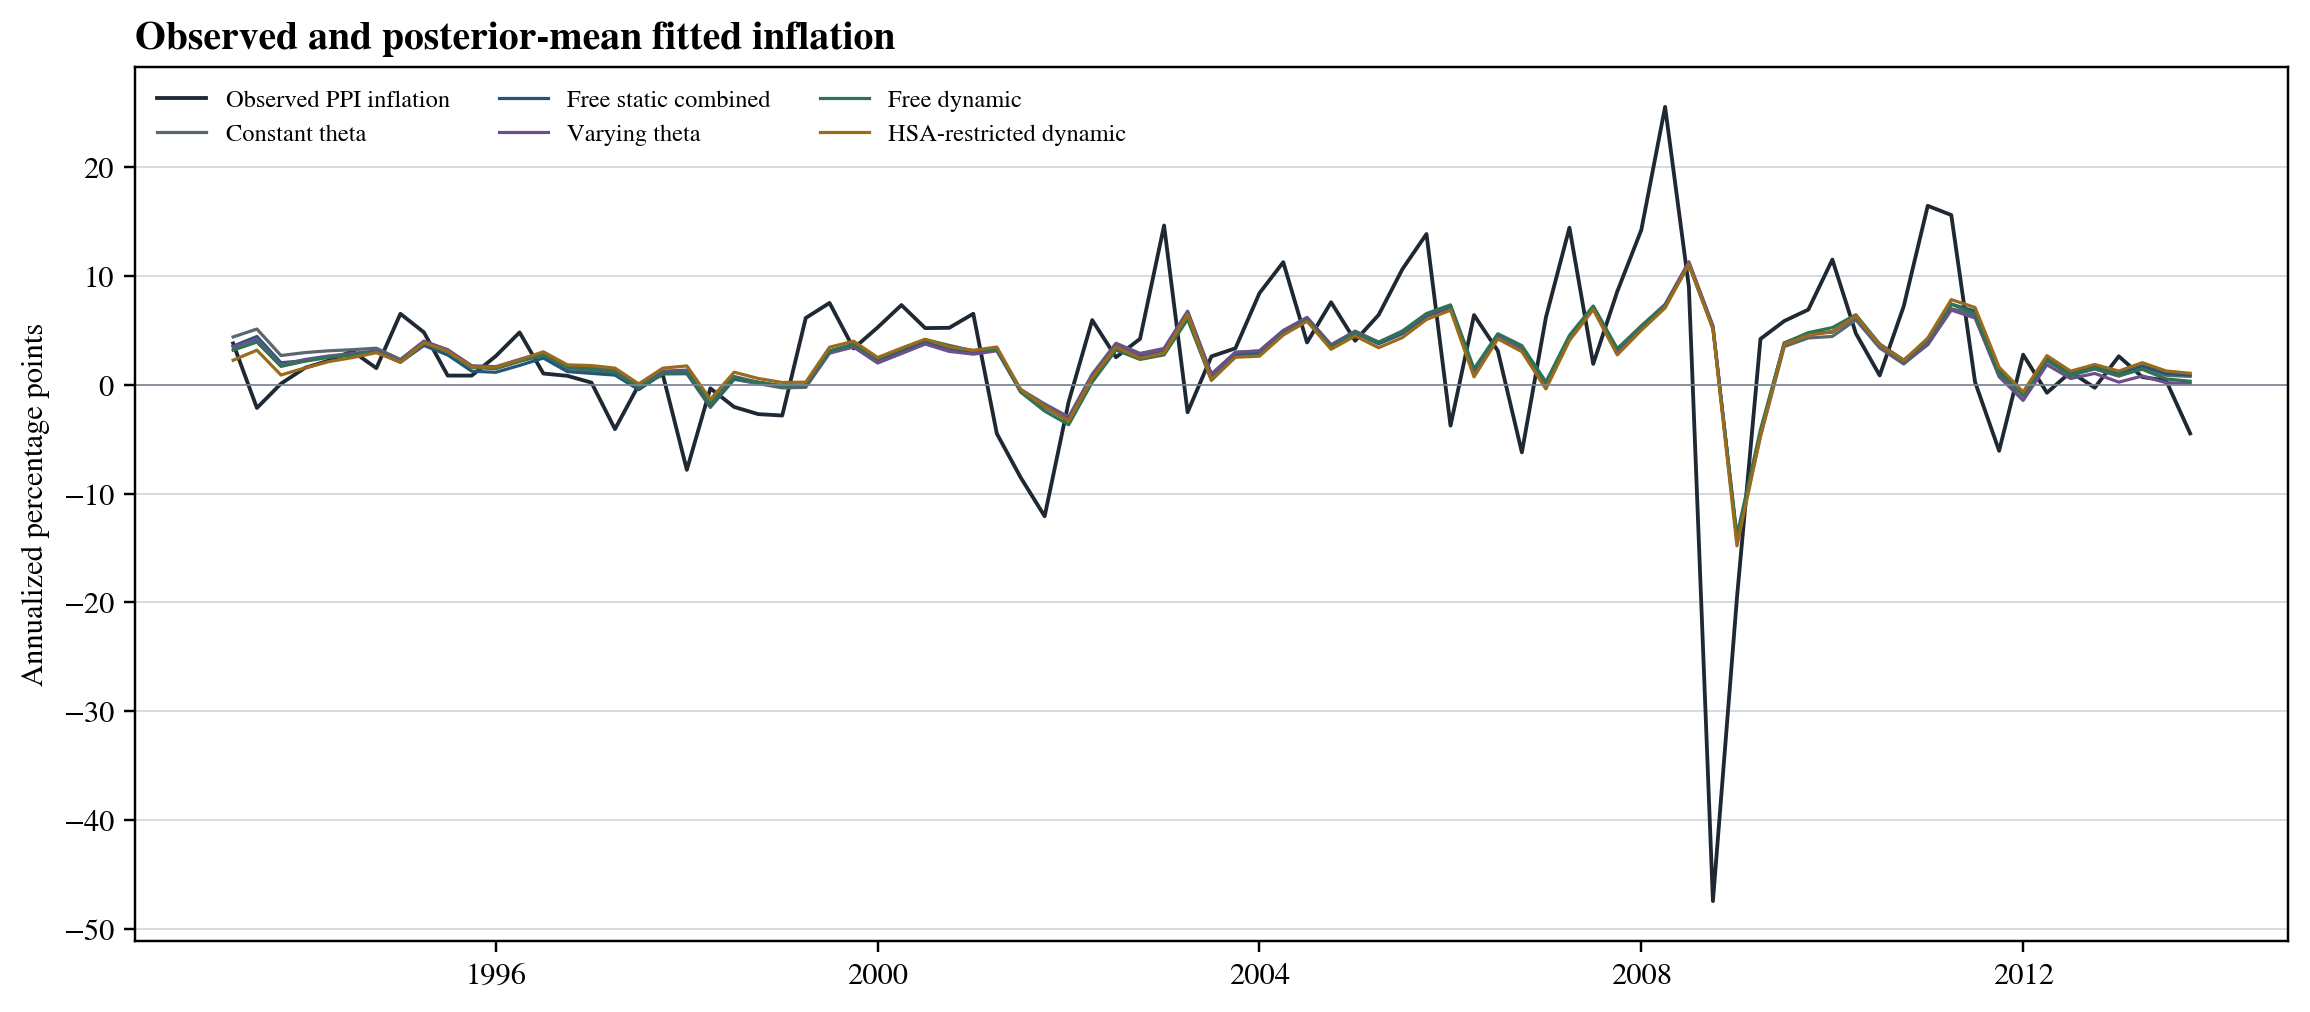
\includegraphics[width=0.92\linewidth]{posterior_fit.png}
\caption{Observed PPI inflation and posterior-mean in-sample fitted values.}
\end{figure}

The fitted means are similar across specifications. Extra dynamic coefficients mostly
redistribute a small fitted competition contribution rather than explaining the large QoQ
inflation movements. This is consistent with the weak predictive gains reported next.

% -----------------------------------------------------------------------------
\section{Model Comparison}

The dynamic models are compared with the constant-theta baseline using full-sample
PSIS-LOO, manually computed WAIC, and a fixed 2010Q1--2013Q4 holdout. Positive ELPD
differences favor the dynamic model; negative RMSE differences favor it.

\begin{table}[H]
\centering
\caption{Dynamic models relative to constant theta}
\resizebox{\linewidth}{!}{\begin{tabular}{@{}lllrrrrr@{}}
\toprule
Cycle & Activity & Model & $\Delta$LOO & $\Delta$WAIC & $\Delta$holdout & $\Delta$RMSE & max $k$ \\
\midrule
firm\_weighted & inverse\_markup & Varying theta & -0.088 & -0.413 & -0.828 & -0.108 & 1.46 \\
firm\_weighted & inverse\_markup & Free dynamic & -0.532 & -0.531 & -1.988 & 0.108 & 1.44 \\
firm\_weighted & inverse\_markup & HSA-restricted dynamic & -0.944 & -0.483 & -1.145 & -0.137 & 1.53 \\
firm\_weighted & negative\_unemployment\_gap & Varying theta & 0.242 & -0.522 & -0.777 & 0.137 & 1.35 \\
firm\_weighted & negative\_unemployment\_gap & Free dynamic & -1.034 & -1.752 & -1.407 & -0.111 & 1.42 \\
firm\_weighted & negative\_unemployment\_gap & HSA-restricted dynamic & -0.270 & -1.213 & -0.636 & -0.274 & 1.58 \\
revenue\_weighted & inverse\_markup & Varying theta & -0.031 & -0.146 & -1.341 & -0.084 & 1.39 \\
revenue\_weighted & inverse\_markup & Free dynamic & -0.135 & -0.661 & -2.444 & 0.082 & 1.43 \\
revenue\_weighted & inverse\_markup & HSA-restricted dynamic & -0.925 & -0.560 & -1.603 & -0.133 & 1.40 \\
revenue\_weighted & negative\_unemployment\_gap & Varying theta & -1.117 & -0.736 & -1.118 & 0.225 & 1.24 \\
revenue\_weighted & negative\_unemployment\_gap & Free dynamic & -2.195 & -0.915 & -1.850 & 0.012 & 1.44 \\
revenue\_weighted & negative\_unemployment\_gap & HSA-restricted dynamic & -1.167 & -0.562 & -0.774 & -0.276 & 1.33 \\
\bottomrule
\end{tabular}
}
\end{table}

All twelve holdout ELPD differences are negative. Some dynamic models reduce holdout RMSE,
but predictive density also evaluates uncertainty and tail behavior; those RMSE gains do not
translate into better predictive distributions. LOO differences are small and unstable.
Every comparison has at least one Pareto $k>0.7$, with maxima above one, so PSIS-LOO is
descriptive only.

\begin{figure}[H]
\centering
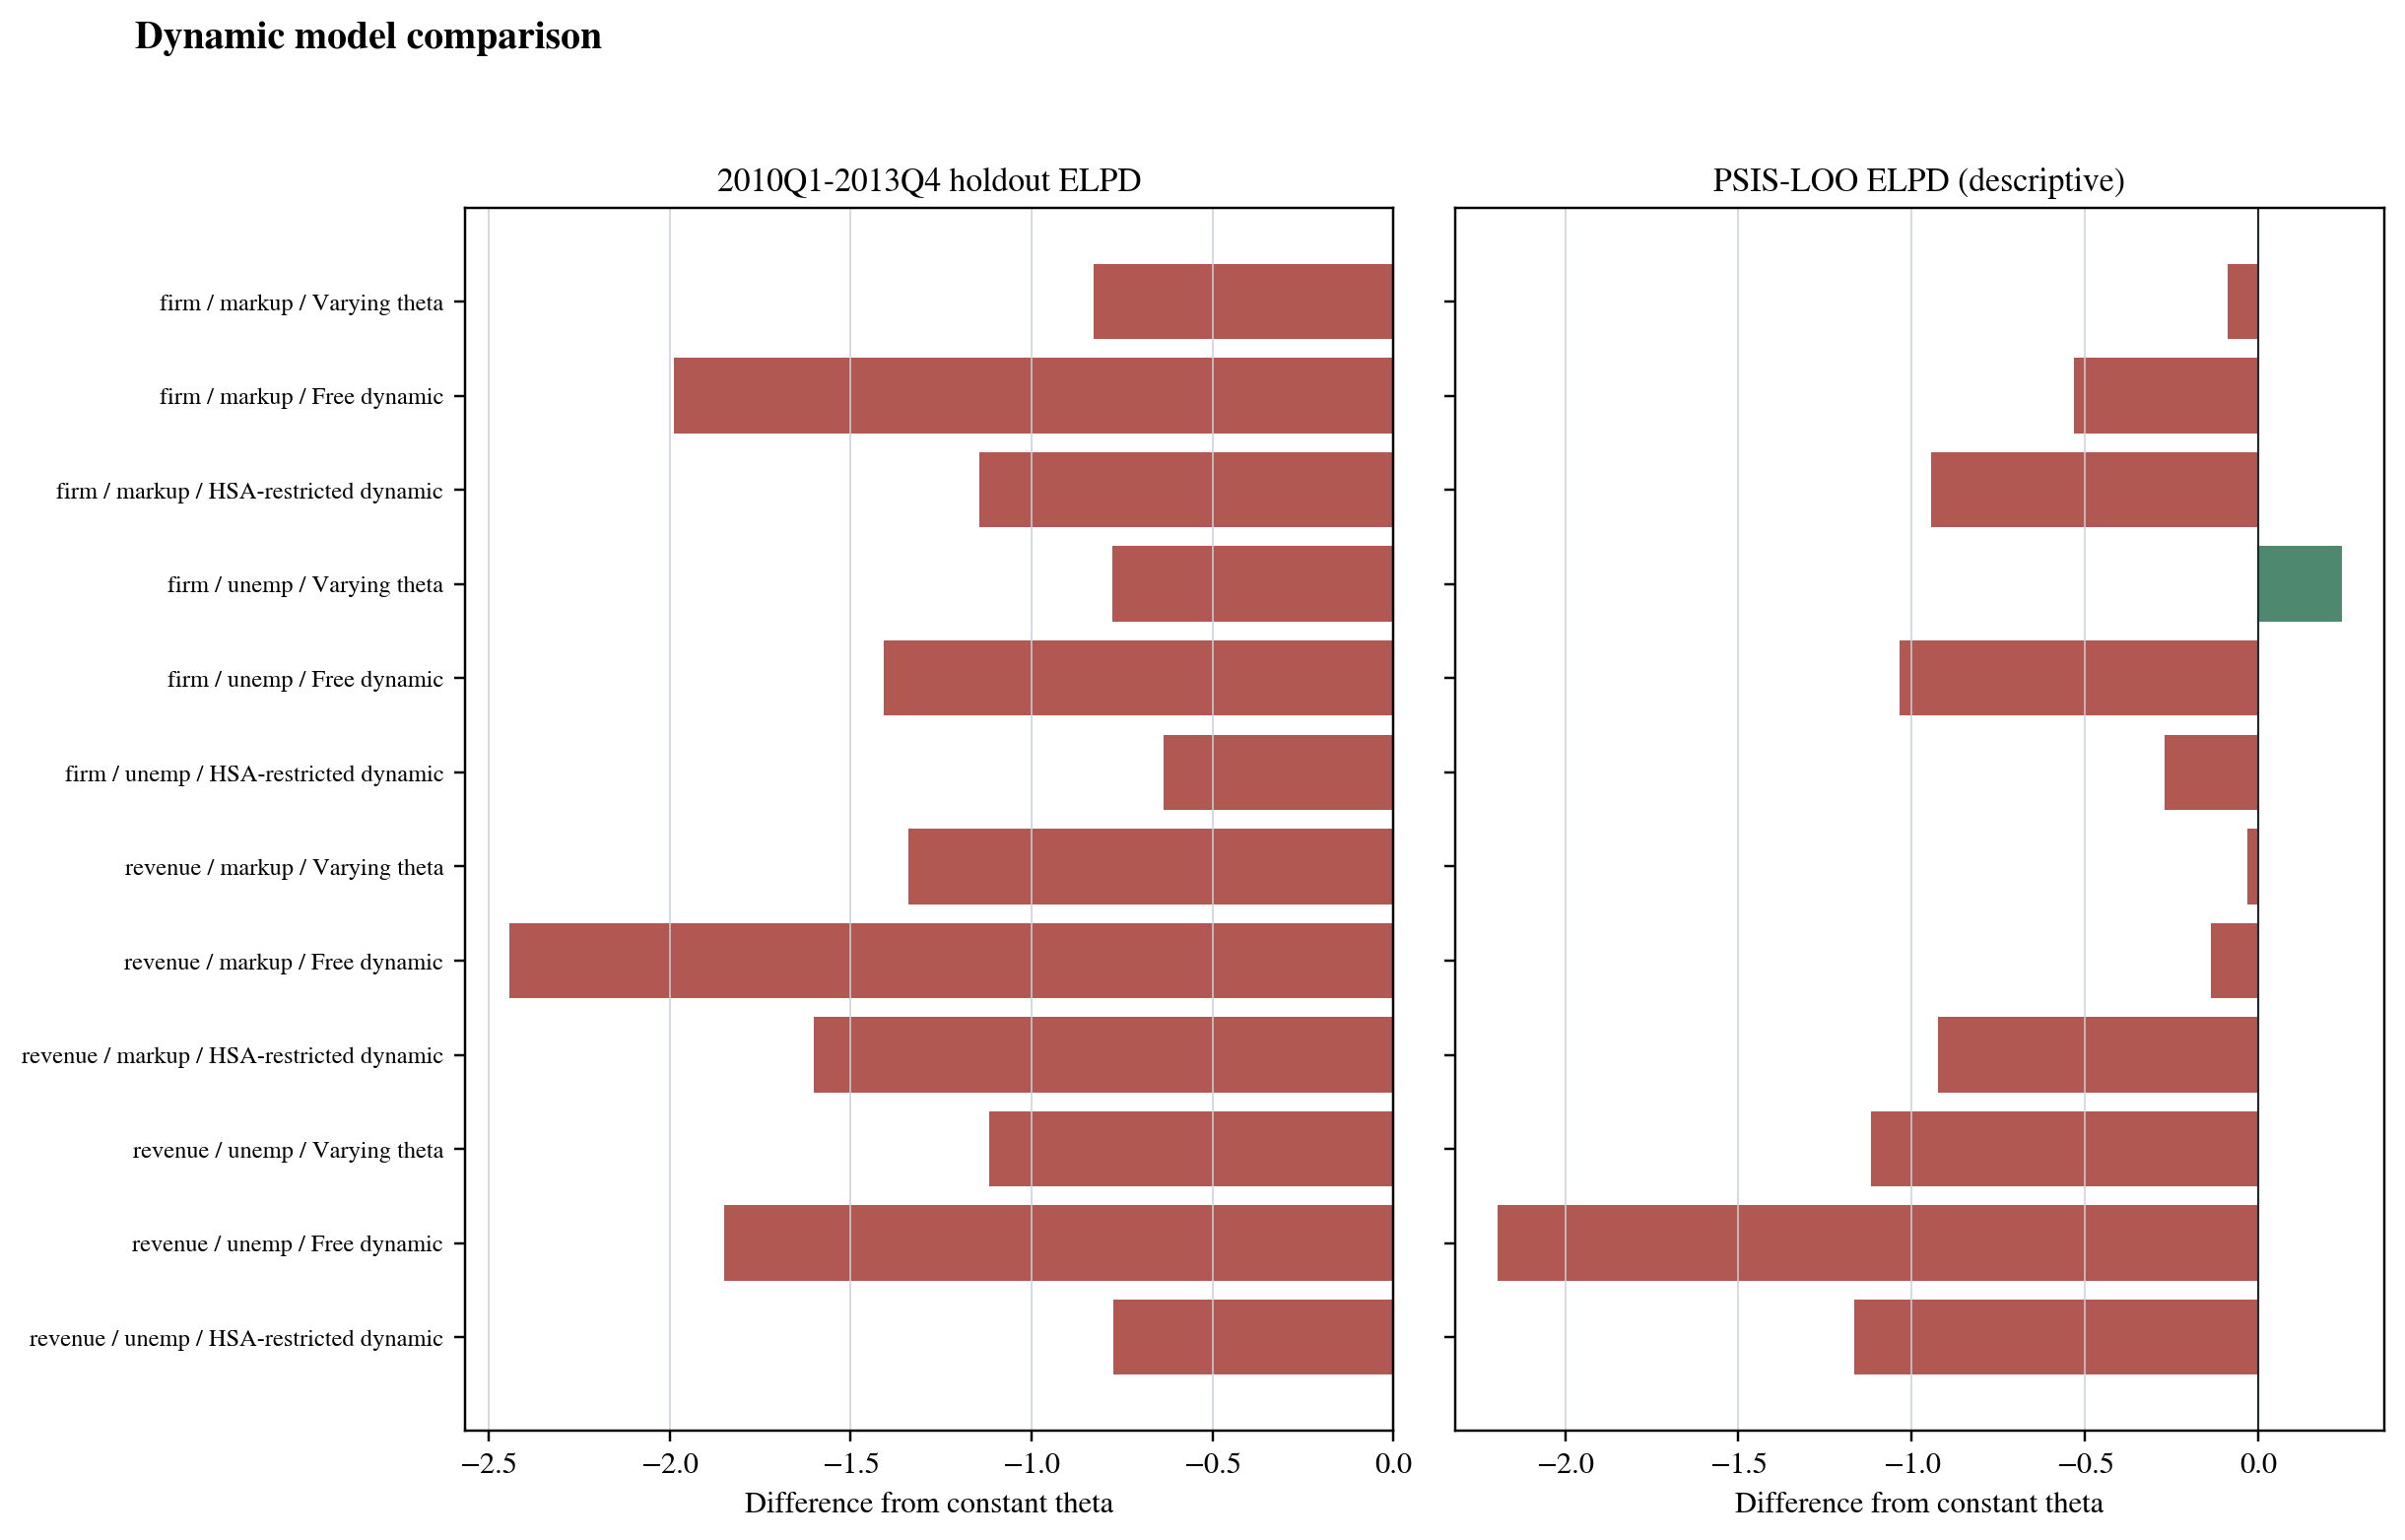
\includegraphics[width=0.94\linewidth]{model_comparison.png}
\caption{Predictive comparison relative to constant theta.}
\end{figure}

No formal marginal likelihood was computed for this post-gate dynamic diagnostic, and the
current QoQ bundle did not re-estimate a separate CES model. Therefore this report does not
make a dynamic-HSA-versus-CES Bayes-factor claim. Its valid nested comparison is free dynamic
versus HSA restricted, with constant theta as the predictive baseline.

% -----------------------------------------------------------------------------
\section{Identification Geometry}

The relevant competition regressors are
\begin{equation}
-\Nhat_t,\quad -\Nbar_t^c\Nhat_t,\quad
\Nbar_t^cx_t,\quad q_t^{(2)}x_t.
\end{equation}
Their standardized condition numbers are not extreme: about 1.0--1.4 for varying theta and
2.3--3.0 for free dynamic. Maximum pairwise correlations are 0.42--0.68. Thus catastrophic
linear collinearity is not the main explanation for failure.

\begin{table}[H]
\centering
\caption{Regressor geometry using posterior-median competition paths}
\resizebox{\linewidth}{!}{\begin{tabular}{@{}lrrrrr@{}}
\toprule
Cell & Corr($\theta_0,\gamma$ regressors) & Corr($\delta_1,\delta_2$ regressors) & Max regressor corr. & Cond. varying & Cond. free dyn. \\
\midrule
Firm / unemployment & 0.296 & -0.423 & 0.601 & 1.36 & 3.03 \\
Revenue / unemployment & -0.009 & -0.393 & 0.676 & 1.01 & 2.96 \\
Firm / inverse markup & 0.296 & 0.388 & 0.416 & 1.36 & 2.34 \\
Revenue / inverse markup & -0.009 & 0.402 & 0.497 & 1.01 & 2.36 \\
\bottomrule
\end{tabular}
}
\end{table}

\begin{table}[H]
\centering
\caption{Posterior dependence among free-dynamic target coefficients}
\begin{tabular}{@{}lr@{}}
\toprule
Cell & Max target posterior correlation \\
\midrule
Firm / unemployment & 0.456 \\
Revenue / unemployment & 0.481 \\
Firm / inverse markup & 0.375 \\
Revenue / inverse markup & 0.391 \\
\bottomrule
\end{tabular}

\end{table}

\begin{figure}[H]
\centering
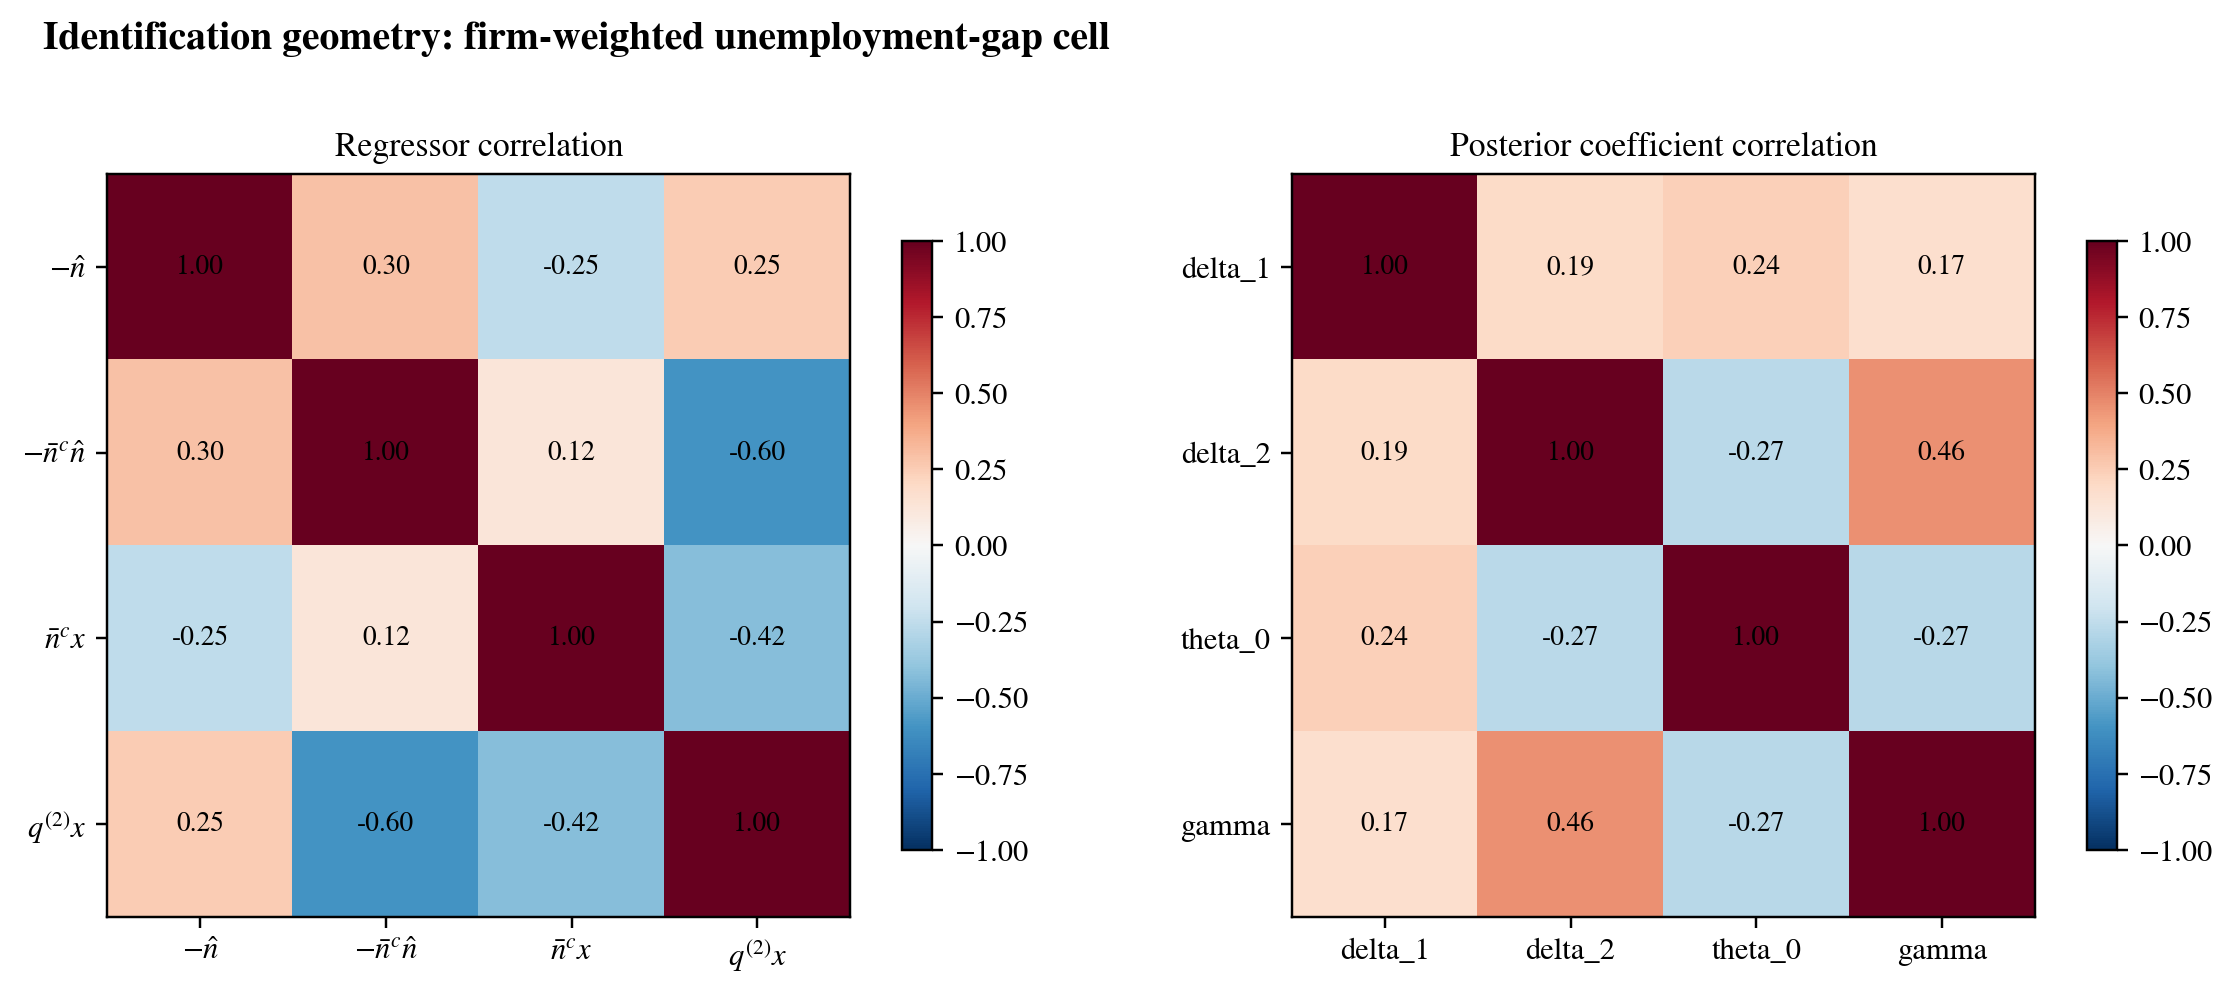
\includegraphics[width=0.86\linewidth]{identification_geometry.png}
\caption{Regressor and posterior correlations in the primary firm-weighted unemployment-gap cell.}
\end{figure}

Posterior target correlations are moderate rather than singular. The problem is primarily
low signal relative to quarterly inflation volatility, limited $T$, and the multiplicative
HSA factorization---not a single near-collinear pair that could be removed to solve the
model.

% -----------------------------------------------------------------------------
\section{Persistent-Error Robustness and MCMC Convergence}

\begin{table}[H]
\centering
\caption{IID versus persistent AR(1), firm-weighted unemployment-gap cell}
\small
\begin{tabular}{@{}llcc@{}}
\toprule
Model & Parameter & IID & Persistent AR(1) \\
\midrule
Varying theta & theta\_0 & \makecell{0.710\\{\scriptsize [-0.865, 2.262]}} & \makecell{0.715\\{\scriptsize [-1.076, 2.543]}} \\
Varying theta & gamma & \makecell{-0.165\\{\scriptsize [-1.030, 0.707]}} & \makecell{-0.158\\{\scriptsize [-1.161, 0.847]}} \\
Free dynamic & delta\_1 & \makecell{0.102\\{\scriptsize [-0.615, 0.851]}} & \makecell{0.069\\{\scriptsize [-0.697, 0.832]}} \\
Free dynamic & delta\_2 & \makecell{-0.177\\{\scriptsize [-1.156, 0.803]}} & \makecell{-0.217\\{\scriptsize [-1.311, 0.866]}} \\
Free dynamic & theta\_0 & \makecell{0.894\\{\scriptsize [-0.845, 2.598]}} & \makecell{0.860\\{\scriptsize [-1.106, 2.782]}} \\
Free dynamic & gamma & \makecell{-0.241\\{\scriptsize [-1.257, 0.746]}} & \makecell{-0.231\\{\scriptsize [-1.338, 0.866]}} \\
HSA-restricted dynamic & theta\_0 & \makecell{0.406\\{\scriptsize [-0.619, 2.035]}} & \makecell{0.351\\{\scriptsize [-0.796, 2.089]}} \\
HSA-restricted dynamic & gamma & \makecell{-0.090\\{\scriptsize [-0.949, 0.721]}} & \makecell{-0.096\\{\scriptsize [-1.113, 0.847]}} \\
HSA-restricted dynamic & lambda & \makecell{0.402\\{\scriptsize [-5.288, 5.952]}} & \makecell{0.401\\{\scriptsize [-5.975, 6.292]}} \\
\bottomrule
\end{tabular}

\end{table}

Allowing persistent inflation errors widens intervals modestly but does not change their
sign conclusions. Free-dynamic $\gamma$ is $-0.231[-1.338,0.866]$ and HSA $\lambda$ is
$0.401[-5.975,6.292]$ under AR(1).

\begin{table}[H]
\centering
\caption{Observed IID fit convergence}
\footnotesize
\begin{tabular}{@{}llrr@{}}
\toprule
Model & Cell & Max R-hat & Min bulk ESS \\
\midrule
Constant theta & Firm / unemployment & 1.0019 & 2466.9 \\
Constant theta & Revenue / unemployment & 1.0008 & 2390.1 \\
Constant theta & Firm / inverse markup & 1.0008 & 2711.9 \\
Constant theta & Revenue / inverse markup & 1.0019 & 2679.6 \\
Free static combined & Firm / unemployment & 1.0011 & 2514.6 \\
Free static combined & Revenue / unemployment & 1.0014 & 2725.2 \\
Free static combined & Firm / inverse markup & 1.0013 & 2592.0 \\
Free static combined & Revenue / inverse markup & 1.0024 & 2654.5 \\
Varying theta & Firm / unemployment & 1.0008 & 6488.6 \\
Varying theta & Revenue / unemployment & 1.0008 & 6832.8 \\
Varying theta & Firm / inverse markup & 1.0003 & 6357.6 \\
Varying theta & Revenue / inverse markup & 1.0007 & 6586.1 \\
Free dynamic & Firm / unemployment & 1.0003 & 6528.4 \\
Free dynamic & Revenue / unemployment & 1.0006 & 6615.1 \\
Free dynamic & Firm / inverse markup & 1.0004 & 6521.4 \\
Free dynamic & Revenue / inverse markup & 1.0005 & 6723.2 \\
HSA-restricted dynamic & Firm / unemployment & 1.0011 & 4569.7 \\
HSA-restricted dynamic & Revenue / unemployment & 1.0005 & 4729.5 \\
HSA-restricted dynamic & Firm / inverse markup & 1.0007 & 4273.2 \\
HSA-restricted dynamic & Revenue / inverse markup & 1.0006 & 4310.0 \\
\bottomrule
\end{tabular}

\end{table}

Every observed fit passes comfortably. Across the dynamic fits, maximum R-hat is 1.0011
and minimum bulk ESS is 4,074.5. Recovery maximum R-hat is 1.0129 and minimum bulk ESS is
498.5. The substantive failure is therefore not an MCMC convergence failure.

\begin{figure}[H]
\centering
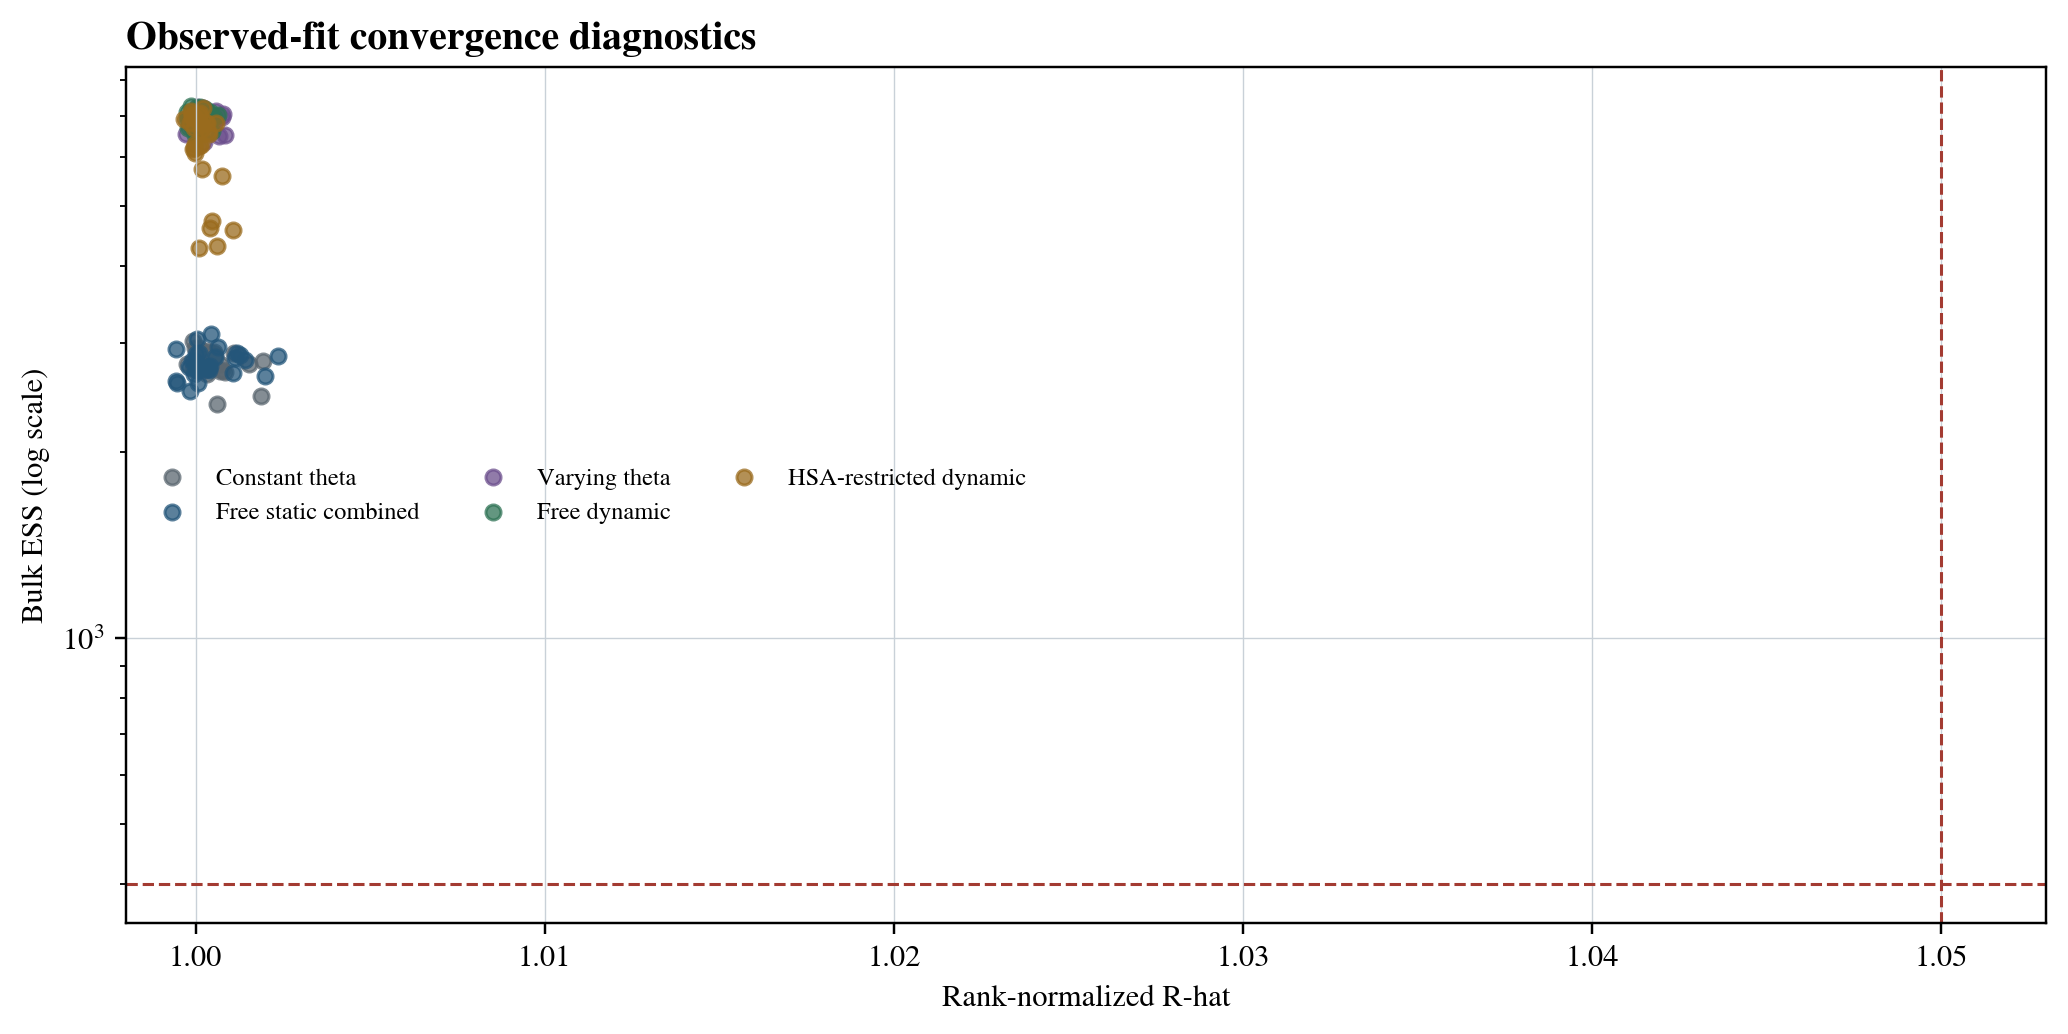
\includegraphics[width=0.82\linewidth]{convergence.png}
\caption{Parameter-level convergence diagnostics. Dashed lines are the dynamic-fit gates.}
\end{figure}

% -----------------------------------------------------------------------------
\section{Core CPI Extension: Matched Data and Design}

Core CPI is estimated as a separate outcome, not pooled with PPI. The competition-state
draws, 1993Q2--2013Q4 sample, activity variables, priors, M0--M4 ladder, IID primary error,
AR(1) robustness, and 2010Q1 holdout are held fixed. The dependent variable is
\begin{equation}
\pi_t^{q,core}=400\left(\log P_t^{core}-\log P_{t-1}^{core}\right),
\end{equation}
where monthly FRED CPILFESL is averaged within quarter before differencing.

The expectation is the Philadelphia Fed SPF mean headline-CPI forecast CPI3. At survey
quarter $t$, CPI3 is the genuine forecast of annualized headline-CPI inflation in $t+1$,
converted to $100\log(1+r_t/100)$. It is horizon-matched and closer to Core CPI than the
GDP-price forecast used for PPI, but it remains a \emph{headline}-CPI proxy because an
independent historical Core-CPI expectation is unavailable.

\begin{table}[H]
\centering
\caption{Core-CPI QoQ data summary}
\resizebox{\linewidth}{!}{\begin{tabular}{@{}p{0.18\linewidth}p{0.18\linewidth}p{0.18\linewidth}cccrr@{}}
\toprule
Series & Source & Transformation & Start & End & $T$ & Mean & SD \\
\midrule
Core CPI inflation & FRED CPILFESL & $400\Delta\log P_t$ & 1993Q2 & 2013Q4 & 83 & 2.155 & 0.644 \\
SPF headline-CPI expectation & Philadelphia Fed CPI3 & $100\log(1+r_t/100)$ & 1993Q2 & 2013Q4 & 83 & 2.304 & 0.571 \\
Negative unemployment gap & FRED NROU and UNRATE & $u_t^*-u_t$ & 1993Q2 & 2013Q4 & 83 & -0.940 & 1.738 \\
Inverse-markup proxy & Nekarda-Ramey markup & $\log(1.2/\mu_t)$ & 1993Q2 & 2013Q4 & 83 & -0.333 & 0.038 \\
\bottomrule
\end{tabular}
}
\end{table}

\begin{figure}[H]
\centering
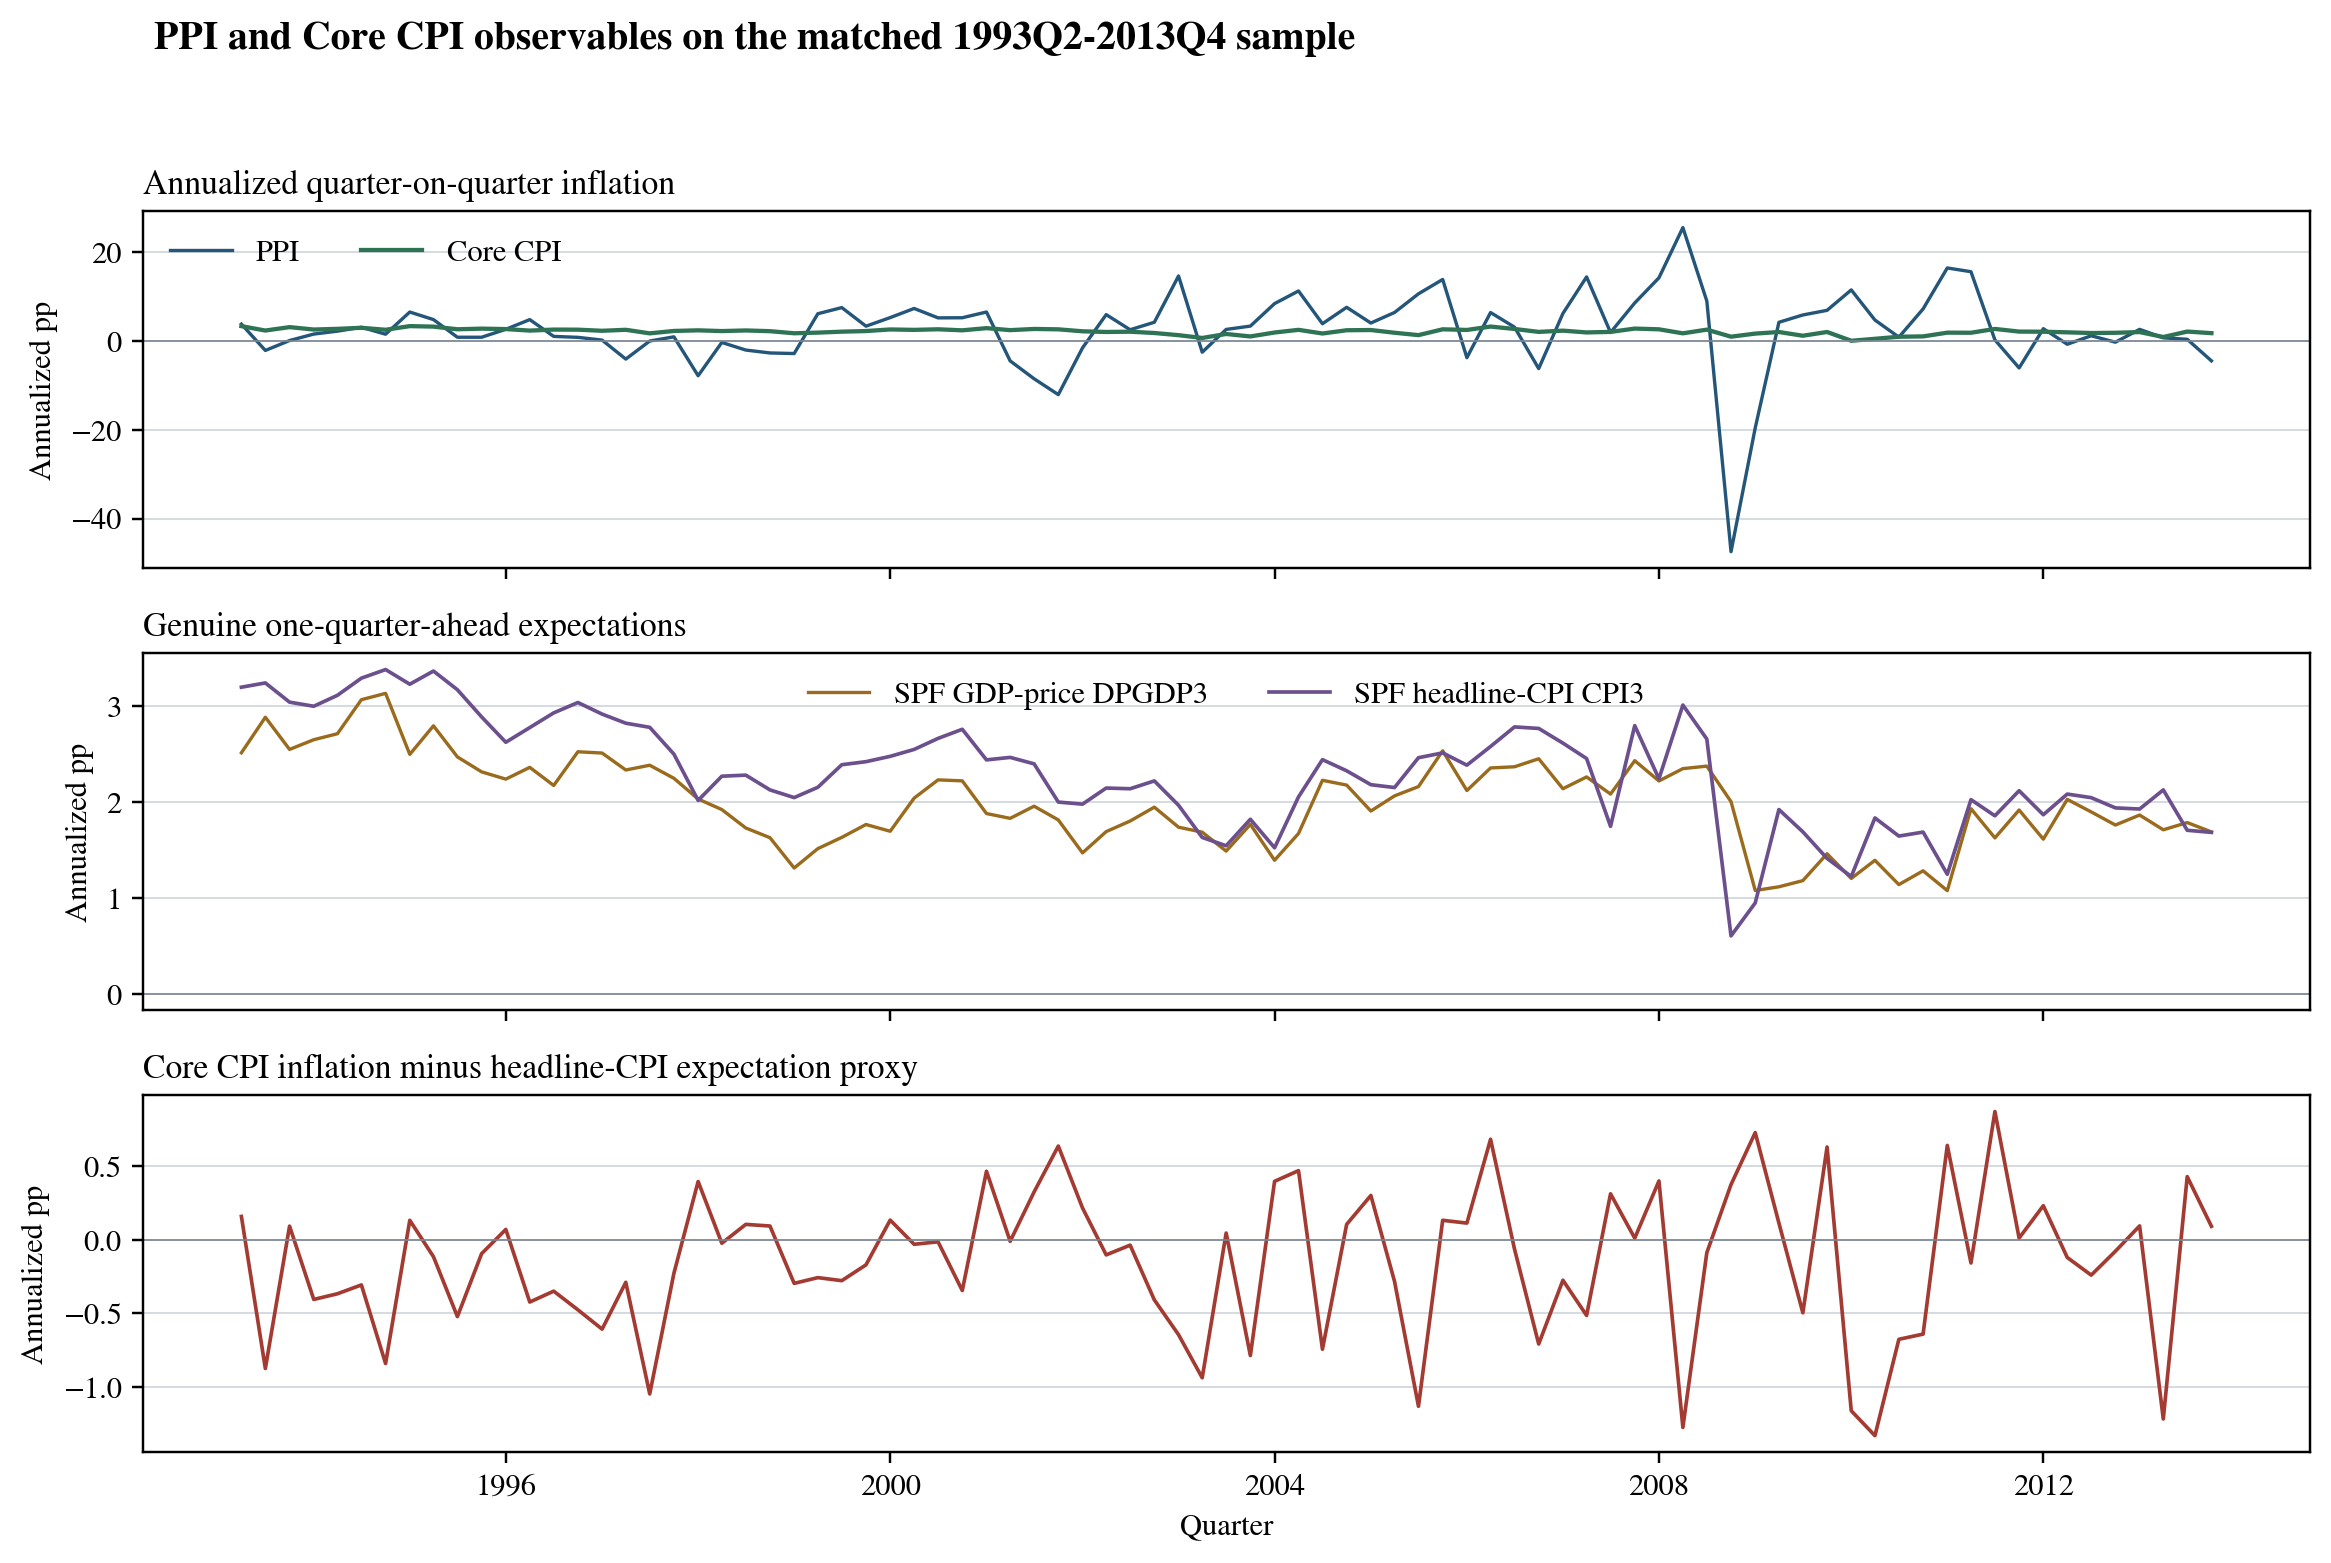
\includegraphics[width=0.91\linewidth]{core_data_timeseries.png}
\caption{Matched PPI and Core-CPI outcomes and their price-appropriate SPF proxies.}
\end{figure}

Core CPI is much smoother than PPI. This changes the signal-to-noise environment and prior
scales, but it does not add observations: both equations still contain only 83 quarters.
The exercise therefore asks whether the PPI direction transports to a less volatile consumer
price outcome, not whether the two inflation series share coefficients.

% -----------------------------------------------------------------------------
\section{Core CPI M0 and M1: Average Direct and Free Static Channels}

For M0 the Core-CPI equation is
\begin{equation}
\pi_t^{q,core}=a+\alpha_b\pi_{t-1}^{q,core}+\alpha_fE_t\pi_{t+1}^{q,CPI}
+\kappa_0x_t-\theta_{CIQ}\Nhat_t+\varepsilon_t.
\end{equation}

\begin{table}[H]
\centering
\caption{Core CPI M0 constant direct loading; posterior mean and 95\% interval}
\resizebox{\linewidth}{!}{\begin{tabular}{@{}lcccc@{}}
\toprule
Parameter & Firm / unemployment & Revenue / unemployment & Firm / inverse markup & Revenue / inverse markup \\
\midrule
alpha\_b & \makecell{0.201\\{\scriptsize [-0.003, 0.406]}} & \makecell{0.200\\{\scriptsize [-0.012, 0.398]}} & \makecell{0.209\\{\scriptsize [-0.006, 0.412]}} & \makecell{0.204\\{\scriptsize [0.002, 0.405]}} \\
alpha\_f & \makecell{0.546\\{\scriptsize [0.314, 0.780]}} & \makecell{0.546\\{\scriptsize [0.300, 0.789]}} & \makecell{0.570\\{\scriptsize [0.335, 0.804]}} & \makecell{0.576\\{\scriptsize [0.338, 0.815]}} \\
kappa\_0 & \makecell{0.042\\{\scriptsize [-0.022, 0.106]}} & \makecell{0.043\\{\scriptsize [-0.022, 0.108]}} & \makecell{1.372\\{\scriptsize [-1.225, 3.908]}} & \makecell{1.415\\{\scriptsize [-1.275, 3.941]}} \\
theta\_CIQ & \makecell{-0.016\\{\scriptsize [-0.111, 0.078]}} & \makecell{-0.016\\{\scriptsize [-0.101, 0.069]}} & \makecell{-0.025\\{\scriptsize [-0.118, 0.067]}} & \makecell{-0.024\\{\scriptsize [-0.112, 0.063]}} \\
\bottomrule
\end{tabular}
}
\end{table}

Unlike PPI, every Core-CPI M0 posterior mean for $\theta_{CIQ}$ is negative. Across the four
cycle/activity cells, $P(\theta_{CIQ}>0)$ is only 0.294--0.378. The posterior SD is
43--46\% of its prior SD, so the sign reversal is not caused by a failure to update. Yet all
four intervals include zero; the result is directional evidence against transportability,
not a sign-identified negative structural effect.

M1 adds the slow-state slope without linking it to the direct loading:
\begin{equation}
\pi_t^{q,core}=\cdots+(\kappa_0+\delta\Nbar_t^c)x_t
-\theta_{CIQ}\Nhat_t+\varepsilon_t.
\end{equation}

\begin{table}[H]
\centering
\caption{Core CPI M1 free-static combined channels}
\resizebox{\linewidth}{!}{\begin{tabular}{@{}lcccc@{}}
\toprule
Parameter & Firm / unemployment & Revenue / unemployment & Firm / inverse markup & Revenue / inverse markup \\
\midrule
kappa\_0 & \makecell{0.024\\{\scriptsize [-0.060, 0.113]}} & \makecell{0.024\\{\scriptsize [-0.058, 0.105]}} & \makecell{1.415\\{\scriptsize [-1.576, 4.273]}} & \makecell{1.438\\{\scriptsize [-1.455, 4.404]}} \\
delta & \makecell{-0.016\\{\scriptsize [-0.067, 0.037]}} & \makecell{-0.019\\{\scriptsize [-0.071, 0.033]}} & \makecell{0.009\\{\scriptsize [-0.227, 0.241]}} & \makecell{0.007\\{\scriptsize [-0.218, 0.237]}} \\
theta\_CIQ & \makecell{-0.029\\{\scriptsize [-0.133, 0.072]}} & \makecell{-0.032\\{\scriptsize [-0.129, 0.069]}} & \makecell{-0.026\\{\scriptsize [-0.124, 0.077]}} & \makecell{-0.023\\{\scriptsize [-0.114, 0.069]}} \\
\bottomrule
\end{tabular}
}
\end{table}

Adding $\delta$ makes the direct mean slightly more negative. In unemployment-gap cells,
$\delta$ also leans negative; in inverse-markup cells it is essentially centered on zero.
Every interval includes zero. Thus M1 does not reveal a hidden positive Core-CPI direct
channel, nor does it identify the standalone slow-slope channel.

% -----------------------------------------------------------------------------
\section{Core CPI M2: Does the Direct Loading Vary?}

The isolated time-variation diagnostic is
\begin{equation}
\pi_t^{q,core}=\cdots+\kappa_0x_t
-(\theta_0+\gamma\Nbar_t^c)\Nhat_t+\varepsilon_t.
\end{equation}

\begin{table}[H]
\centering
\caption{Core CPI M2 varying-theta model}
\resizebox{\linewidth}{!}{\begin{tabular}{@{}lcccc@{}}
\toprule
Parameter & Firm / unemployment & Revenue / unemployment & Firm / inverse markup & Revenue / inverse markup \\
\midrule
kappa\_0 & \makecell{0.056\\{\scriptsize [-0.013, 0.125]}} & \makecell{0.057\\{\scriptsize [-0.015, 0.129]}} & \makecell{1.647\\{\scriptsize [-1.120, 4.385]}} & \makecell{1.725\\{\scriptsize [-0.950, 4.535]}} \\
theta\_0 & \makecell{-0.026\\{\scriptsize [-0.121, 0.069]}} & \makecell{-0.016\\{\scriptsize [-0.104, 0.073]}} & \makecell{-0.035\\{\scriptsize [-0.134, 0.060]}} & \makecell{-0.023\\{\scriptsize [-0.113, 0.066]}} \\
gamma & \makecell{0.030\\{\scriptsize [-0.025, 0.087]}} & \makecell{0.025\\{\scriptsize [-0.027, 0.078]}} & \makecell{0.022\\{\scriptsize [-0.032, 0.077]}} & \makecell{0.018\\{\scriptsize [-0.032, 0.067]}} \\
\bottomrule
\end{tabular}
}
\end{table}

$\theta_0$ retains the negative M0 direction. By contrast, every $\gamma$ mean is positive.
The strongest directional cell is firm-weighted Core CPI $\times$ unemployment gap,
$\gamma=0.030[-0.025,0.087]$ with $P(\gamma>0)=0.860$. The revenue-weighted version gives
$0.025[-0.027,0.078]$ with probability 0.829. This pattern is worth reporting, but it does
not meet interval or recovery criteria and therefore cannot be described as identified
time variation.

% -----------------------------------------------------------------------------
\section{Core CPI M3 and M4: Free Dynamic versus HSA Dynamic}

The unrestricted M3 benchmark estimates
\begin{equation}
\theta_t=\theta_0+\gamma\Nbar_t^c,\qquad
\kappa_t=\kappa_0+\delta_1\Nbar_t^c+\delta_2q_t^{(2)}.
\end{equation}

\begin{table}[H]
\centering
\caption{Core CPI M3 free-dynamic model}
\resizebox{\linewidth}{!}{\begin{tabular}{@{}lcccc@{}}
\toprule
Parameter & Firm / unemployment & Revenue / unemployment & Firm / inverse markup & Revenue / inverse markup \\
\midrule
kappa\_0 & \makecell{0.039\\{\scriptsize [-0.053, 0.128]}} & \makecell{0.037\\{\scriptsize [-0.054, 0.129]}} & \makecell{1.233\\{\scriptsize [-2.147, 4.604]}} & \makecell{1.234\\{\scriptsize [-2.265, 4.732]}} \\
delta\_1 & \makecell{-0.023\\{\scriptsize [-0.081, 0.034]}} & \makecell{-0.024\\{\scriptsize [-0.081, 0.032]}} & \makecell{-0.038\\{\scriptsize [-0.306, 0.223]}} & \makecell{-0.044\\{\scriptsize [-0.310, 0.217]}} \\
delta\_2 & \makecell{-0.024\\{\scriptsize [-0.097, 0.048]}} & \makecell{-0.020\\{\scriptsize [-0.096, 0.056]}} & \makecell{0.040\\{\scriptsize [-0.117, 0.201]}} & \makecell{0.043\\{\scriptsize [-0.124, 0.209]}} \\
theta\_0 & \makecell{-0.028\\{\scriptsize [-0.138, 0.088]}} & \makecell{-0.025\\{\scriptsize [-0.128, 0.079]}} & \makecell{-0.042\\{\scriptsize [-0.143, 0.060]}} & \makecell{-0.031\\{\scriptsize [-0.126, 0.069]}} \\
gamma & \makecell{0.018\\{\scriptsize [-0.048, 0.083]}} & \makecell{0.015\\{\scriptsize [-0.047, 0.078]}} & \makecell{0.026\\{\scriptsize [-0.030, 0.082]}} & \makecell{0.020\\{\scriptsize [-0.033, 0.072]}} \\
\bottomrule
\end{tabular}
}
\end{table}

All M3 intervals for $\delta_1,\delta_2,\theta_0$, and $\gamma$ include zero. The markup
cells lean toward $\delta_2>0$ and $\gamma>0$, while the unemployment-gap cells lean toward
negative slope changes. These differences show why a restriction should not be credited
with identification before the free coefficients are recovered.

M4 imposes the HSA cross-equation restriction:
\begin{align}
\pi_t^{q,core}={}&a+\alpha_b\pi_{t-1}^{q,core}+\alpha_fE_t\pi_{t+1}^{q,CPI}\\
&+\left(\kappa_0+\lambda\theta_0\Nbar_t^c
+\frac{\lambda\gamma}{2}q_t^{(2)}\right)x_t\\
&-(\theta_0+\gamma\Nbar_t^c)\Nhat_t+\varepsilon_t.
\end{align}

\begin{table}[H]
\centering
\caption{Core CPI M4 HSA-restricted dynamic model}
\resizebox{0.94\linewidth}{!}{\begin{tabular}{@{}lcccc@{}}
\toprule
Parameter & Firm / unemployment & Revenue / unemployment & Firm / inverse markup & Revenue / inverse markup \\
\midrule
kappa\_0 & \makecell{0.030\\{\scriptsize [-0.074, 0.125]}} & \makecell{0.029\\{\scriptsize [-0.074, 0.120]}} & \makecell{1.174\\{\scriptsize [-2.651, 4.617]}} & \makecell{1.265\\{\scriptsize [-2.422, 4.602]}} \\
theta\_0 & \makecell{-0.016\\{\scriptsize [-0.111, 0.044]}} & \makecell{-0.015\\{\scriptsize [-0.105, 0.046]}} & \makecell{-0.028\\{\scriptsize [-0.112, 0.047]}} & \makecell{-0.019\\{\scriptsize [-0.093, 0.051]}} \\
gamma & \makecell{0.009\\{\scriptsize [-0.057, 0.071]}} & \makecell{0.008\\{\scriptsize [-0.055, 0.067]}} & \makecell{0.023\\{\scriptsize [-0.029, 0.080]}} & \makecell{0.019\\{\scriptsize [-0.029, 0.070]}} \\
lambda & \makecell{0.564\\{\scriptsize [-8.287, 9.120]}} & \makecell{0.775\\{\scriptsize [-7.771, 9.291]}} & \makecell{1.056\\{\scriptsize [-10.042, 11.710]}} & \makecell{1.185\\{\scriptsize [-10.358, 12.916]}} \\
derived:delta\_1 & \makecell{-0.027\\{\scriptsize [-0.114, 0.031]}} & \makecell{-0.027\\{\scriptsize [-0.109, 0.033]}} & \makecell{-0.054\\{\scriptsize [-0.429, 0.243]}} & \makecell{-0.049\\{\scriptsize [-0.422, 0.225]}} \\
derived:delta\_2 & \makecell{-0.019\\{\scriptsize [-0.112, 0.030]}} & \makecell{-0.015\\{\scriptsize [-0.108, 0.036]}} & \makecell{0.028\\{\scriptsize [-0.096, 0.214]}} & \makecell{0.028\\{\scriptsize [-0.091, 0.228]}} \\
\bottomrule
\end{tabular}
}
\end{table}

Every $\lambda$ interval spans both signs. In the firm-weighted unemployment-gap cell,
$\lambda=0.564[-8.287,9.120]$; in the corresponding inverse-markup cell it is
$1.056[-10.042,11.710]$. All derived $\delta_1=\lambda\theta_0$ and
$\delta_2=\lambda\gamma/2$ intervals include zero. As in PPI, posterior narrowing inside
M4 reflects shared multiplicative restrictions and is not independent evidence for the
direct channel.

% -----------------------------------------------------------------------------
\section{PPI versus Core CPI: Coefficients on a Common Layout}

The following table holds the Capital IQ aggregation fixed at firm weighting and places the
two inflation outcomes and two activity measures in columns. The equations are exactly M0--M4
above; only $\pi_t$, its lag, and its expectation proxy change across price indices.

\begin{table}[H]
\centering
\caption{Firm-weighted target coefficients across PPI and Core CPI}
\scriptsize
\begin{tabular}{@{}lcccc@{}}
\toprule
Target & PPI / unemployment & PPI / inverse markup & Core CPI / unemployment & Core CPI / inverse markup \\
\midrule
M0 $\theta$ & \makecell{0.674\\{\scriptsize [-0.845, 2.200]}} & \makecell{0.656\\{\scriptsize [-0.843, 2.176]}} & \makecell{-0.016\\{\scriptsize [-0.111, 0.078]}} & \makecell{-0.025\\{\scriptsize [-0.118, 0.067]}} \\
M1 $\delta$ & \makecell{0.173\\{\scriptsize [-0.517, 0.861]}} & \makecell{0.221\\{\scriptsize [-2.779, 3.255]}} & \makecell{-0.016\\{\scriptsize [-0.067, 0.037]}} & \makecell{0.009\\{\scriptsize [-0.227, 0.241]}} \\
M1 $\theta$ & \makecell{0.784\\{\scriptsize [-0.832, 2.388]}} & \makecell{0.672\\{\scriptsize [-0.874, 2.189]}} & \makecell{-0.029\\{\scriptsize [-0.133, 0.072]}} & \makecell{-0.026\\{\scriptsize [-0.124, 0.077]}} \\
M2 $\theta_0$ & \makecell{0.710\\{\scriptsize [-0.865, 2.262]}} & \makecell{0.749\\{\scriptsize [-0.813, 2.283]}} & \makecell{-0.026\\{\scriptsize [-0.121, 0.069]}} & \makecell{-0.035\\{\scriptsize [-0.134, 0.060]}} \\
M2 $\gamma$ & \makecell{-0.165\\{\scriptsize [-1.030, 0.707]}} & \makecell{-0.215\\{\scriptsize [-1.083, 0.645]}} & \makecell{0.030\\{\scriptsize [-0.025, 0.087]}} & \makecell{0.022\\{\scriptsize [-0.032, 0.077]}} \\
M3 $\delta_1$ & \makecell{0.102\\{\scriptsize [-0.615, 0.851]}} & \makecell{-0.076\\{\scriptsize [-3.463, 3.262]}} & \makecell{-0.023\\{\scriptsize [-0.081, 0.034]}} & \makecell{-0.038\\{\scriptsize [-0.306, 0.223]}} \\
M3 $\delta_2$ & \makecell{-0.177\\{\scriptsize [-1.156, 0.803]}} & \makecell{0.813\\{\scriptsize [-1.530, 3.137]}} & \makecell{-0.024\\{\scriptsize [-0.097, 0.048]}} & \makecell{0.040\\{\scriptsize [-0.117, 0.201]}} \\
M3 $\theta_0$ & \makecell{0.894\\{\scriptsize [-0.845, 2.598]}} & \makecell{0.613\\{\scriptsize [-0.993, 2.296]}} & \makecell{-0.028\\{\scriptsize [-0.138, 0.088]}} & \makecell{-0.042\\{\scriptsize [-0.143, 0.060]}} \\
M3 $\gamma$ & \makecell{-0.241\\{\scriptsize [-1.257, 0.746]}} & \makecell{-0.191\\{\scriptsize [-1.064, 0.693]}} & \makecell{0.018\\{\scriptsize [-0.048, 0.083]}} & \makecell{0.026\\{\scriptsize [-0.030, 0.082]}} \\
M4 $\theta_0$ & \makecell{0.406\\{\scriptsize [-0.619, 2.035]}} & \makecell{0.375\\{\scriptsize [-0.664, 1.832]}} & \makecell{-0.016\\{\scriptsize [-0.111, 0.044]}} & \makecell{-0.028\\{\scriptsize [-0.112, 0.047]}} \\
M4 $\gamma$ & \makecell{-0.090\\{\scriptsize [-0.949, 0.721]}} & \makecell{-0.175\\{\scriptsize [-0.996, 0.668]}} & \makecell{0.009\\{\scriptsize [-0.057, 0.071]}} & \makecell{0.023\\{\scriptsize [-0.029, 0.080]}} \\
M4 $\lambda$ & \makecell{0.402\\{\scriptsize [-5.288, 5.952]}} & \makecell{-0.411\\{\scriptsize [-13.298, 12.196]}} & \makecell{0.564\\{\scriptsize [-8.287, 9.120]}} & \makecell{1.056\\{\scriptsize [-10.042, 11.710]}} \\
M4 $\delta_1$ & \makecell{0.149\\{\scriptsize [-0.644, 1.033]}} & \makecell{-0.028\\{\scriptsize [-3.901, 3.895]}} & \makecell{-0.027\\{\scriptsize [-0.114, 0.031]}} & \makecell{-0.054\\{\scriptsize [-0.429, 0.243]}} \\
M4 $\delta_2$ & \makecell{-0.016\\{\scriptsize [-0.705, 0.615]}} & \makecell{0.427\\{\scriptsize [-1.181, 3.065]}} & \makecell{-0.019\\{\scriptsize [-0.112, 0.030]}} & \makecell{0.028\\{\scriptsize [-0.096, 0.214]}} \\
\bottomrule
\end{tabular}

\end{table}

The comparison makes the central result visible. PPI M0/M1 $\theta$ means are positive,
whereas Core-CPI means are negative. PPI $\gamma$ leans negative, whereas Core-CPI $\gamma$
leans positive. No corresponding 95\% interval excludes zero. Consequently the cross-price
exercise weakens, rather than strengthens, a claim of a common HSA coefficient. Pooling the
two price systems would conceal this economically relevant heterogeneity.

% -----------------------------------------------------------------------------
\section{Core CPI Prior--Posterior Learning and Recovery}

\begin{figure}[H]
\centering
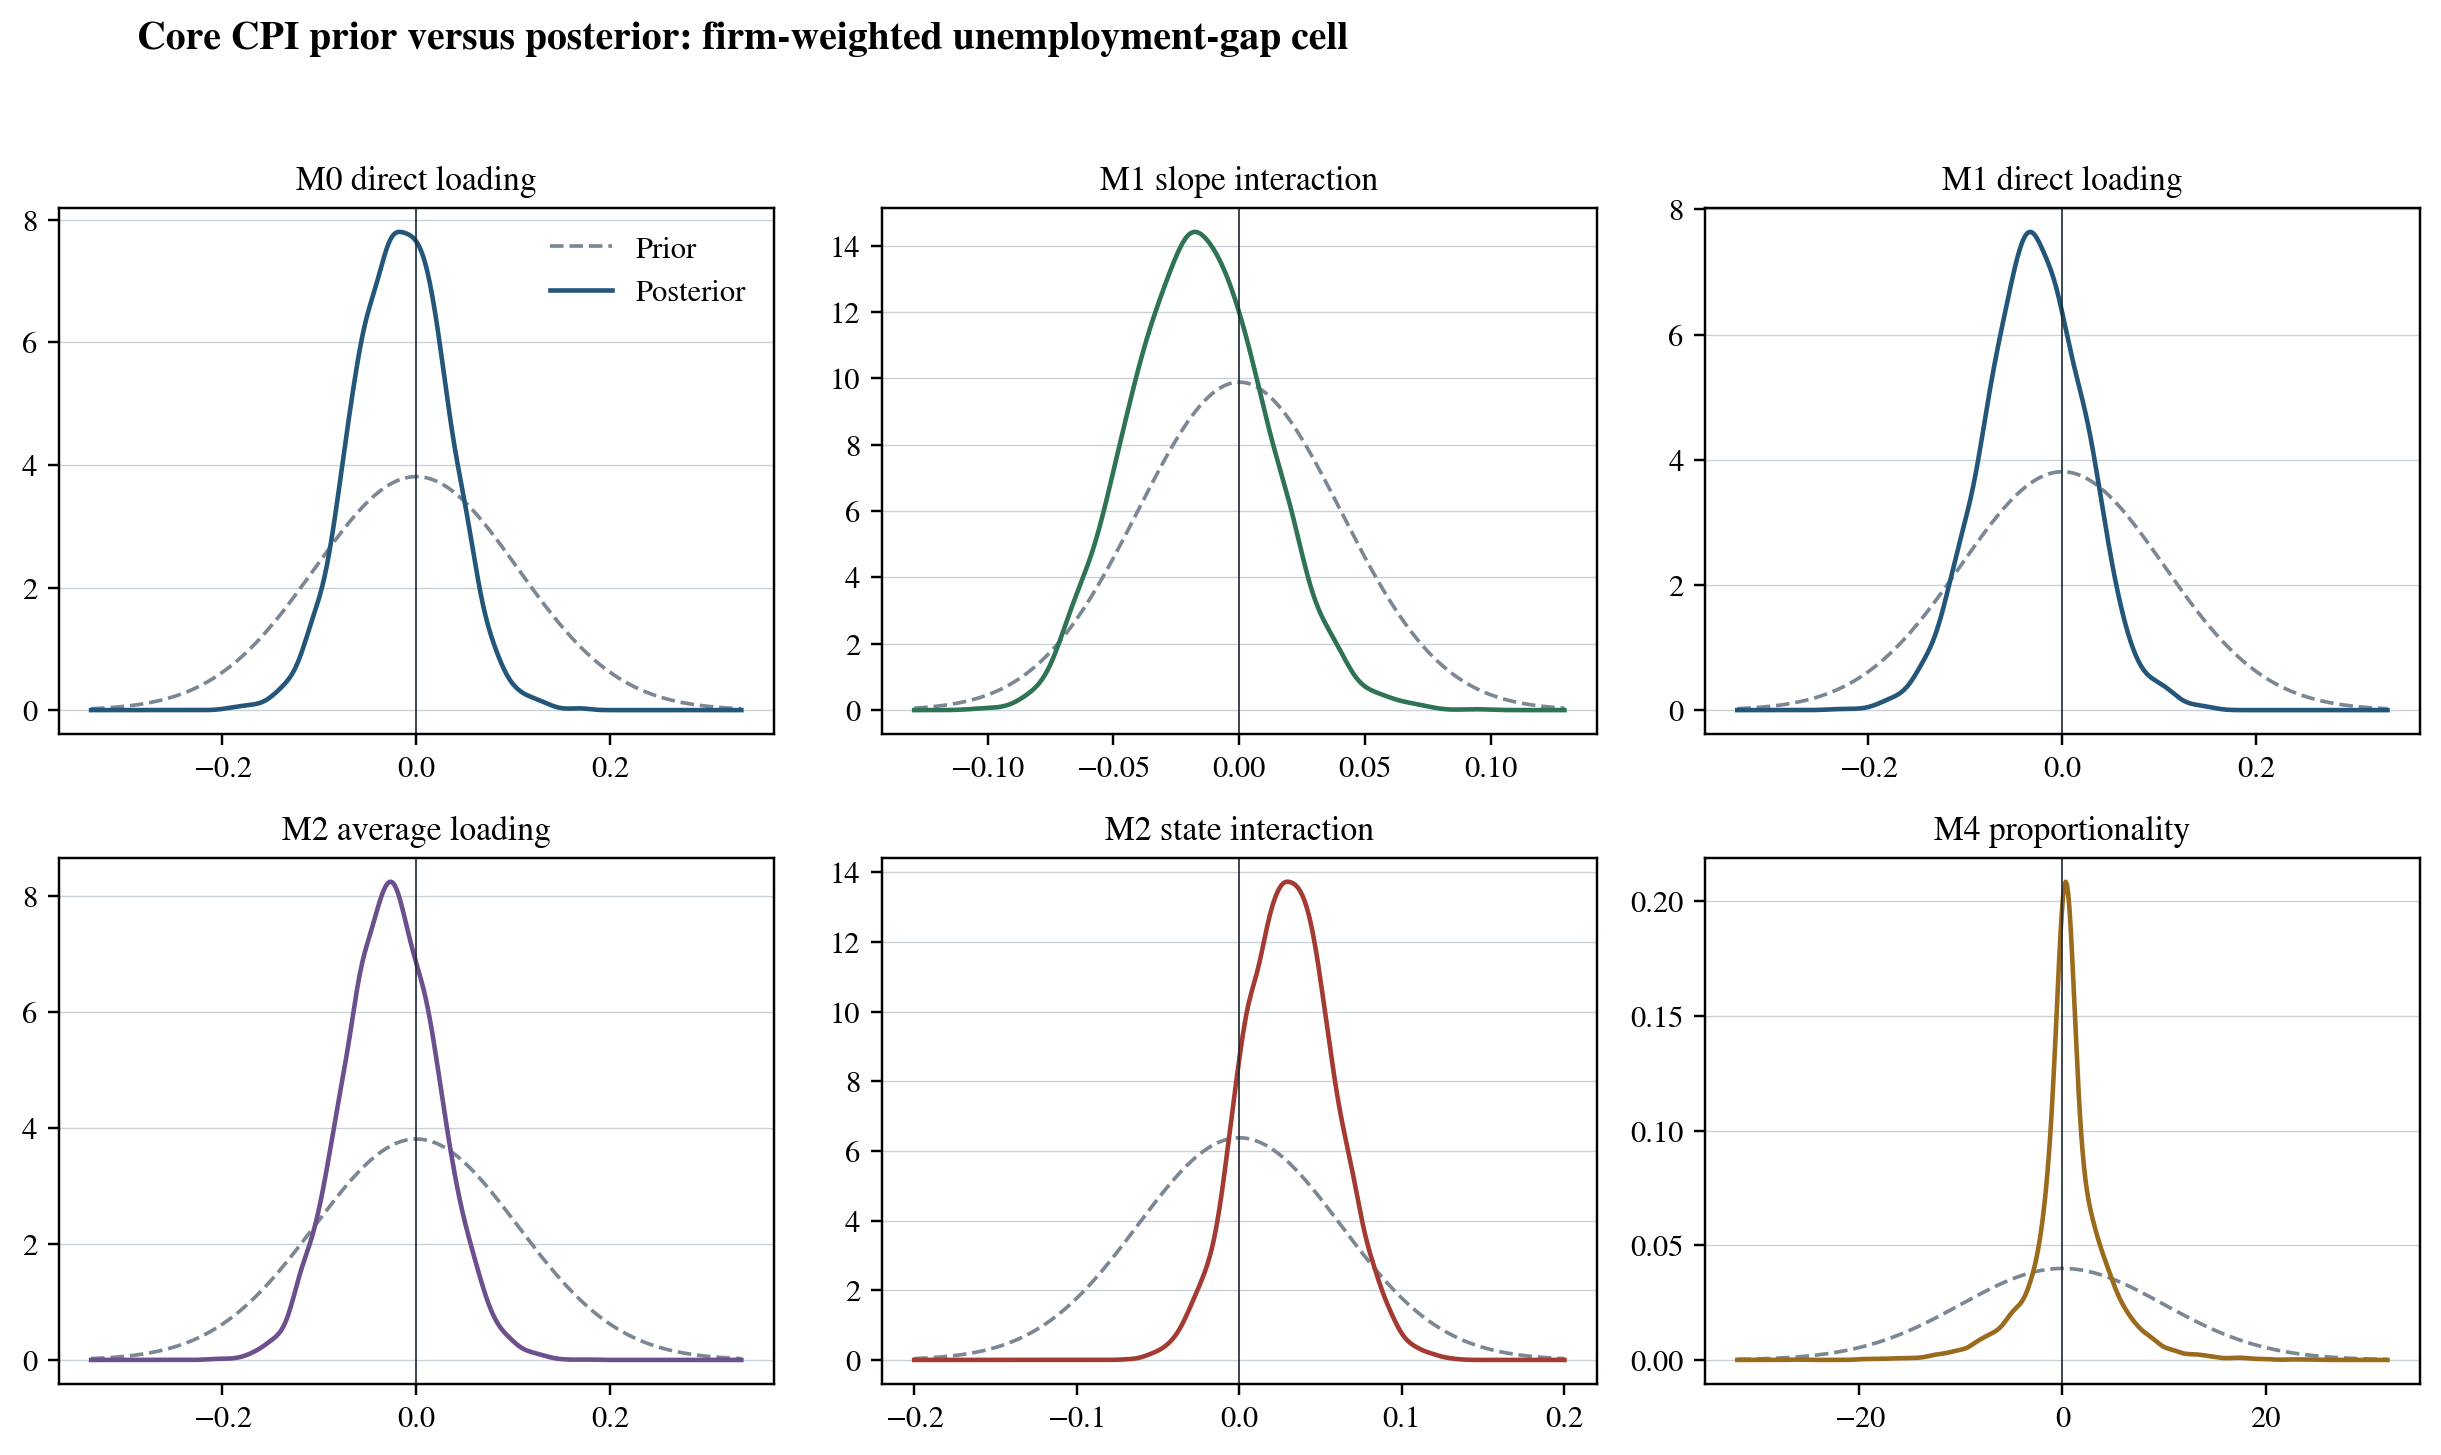
\includegraphics[width=0.91\linewidth]{core_prior_posterior.png}
\caption{Core CPI selected prior-versus-posterior densities.}
\end{figure}

The posteriors narrow substantially relative to their standardized priors. This is genuine
Bayesian learning about the empirical regressions. It is nevertheless distinct from learning
the theoretically maintained sign: a narrow posterior can lie mostly on the opposite side of
zero, and every reported interval can still span zero.

The Core-CPI recovery experiment repeats the PPI grids on the actual Core-CPI outcome,
activity paths, persistence, and frozen state draws. It contains 480 static and 300 dynamic
fits, with 30 propagated-state and 30 oracle-state replications per injected effect.

\begin{table}[H]
\centering
\caption{Core CPI propagated-state free-static recovery}
\begin{tabular}{@{}llrrrr@{}}
\toprule
Scenario & Parameter & True effect & Suggestive & Strong & Coverage \\
\midrule
both\_observed & delta & 0.06 & 0.000 & 0.000 & 1.000 \\
both\_observed & theta\_CIQ & 0.11 & 0.433 & 0.067 & 0.967 \\
both\_moderate & delta & 0.20 & 0.200 & 0.000 & 0.867 \\
both\_moderate & theta\_CIQ & 0.20 & 0.767 & 0.033 & 0.933 \\
both\_large & delta & 0.40 & 0.833 & 0.033 & 0.567 \\
both\_large & theta\_CIQ & 0.40 & 0.867 & 0.500 & 0.567 \\
\bottomrule
\end{tabular}

\end{table}

At $(s_\delta,s_\theta)=(0.06,0.11)$, suggestive recovery is 0 for $\delta$ and 0.433 for
$\theta$. Oracle-state rates are 0.067 and 0.500. At $s_\gamma=0.10$, propagated-state
suggestive recovery is 0.367 and strong recovery is 0.067.

\begin{table}[H]
\centering
\caption{Core CPI propagated-state recovery of $\gamma$}
\begin{tabular}{@{}rrrrr@{}}
\toprule
True $s_\gamma$ & Suggestive & Strong & Coverage & Mean SD ratio \\
\midrule
0.00 & 0.000 & 0.000 & 0.967 & 0.438 \\
0.05 & 0.200 & 0.000 & 1.000 & 0.436 \\
0.10 & 0.367 & 0.067 & 0.933 & 0.449 \\
0.20 & 0.867 & 0.367 & 0.967 & 0.460 \\
0.40 & 1.000 & 0.767 & 0.733 & 0.485 \\
\bottomrule
\end{tabular}

\end{table}

\begin{figure}[H]
\centering
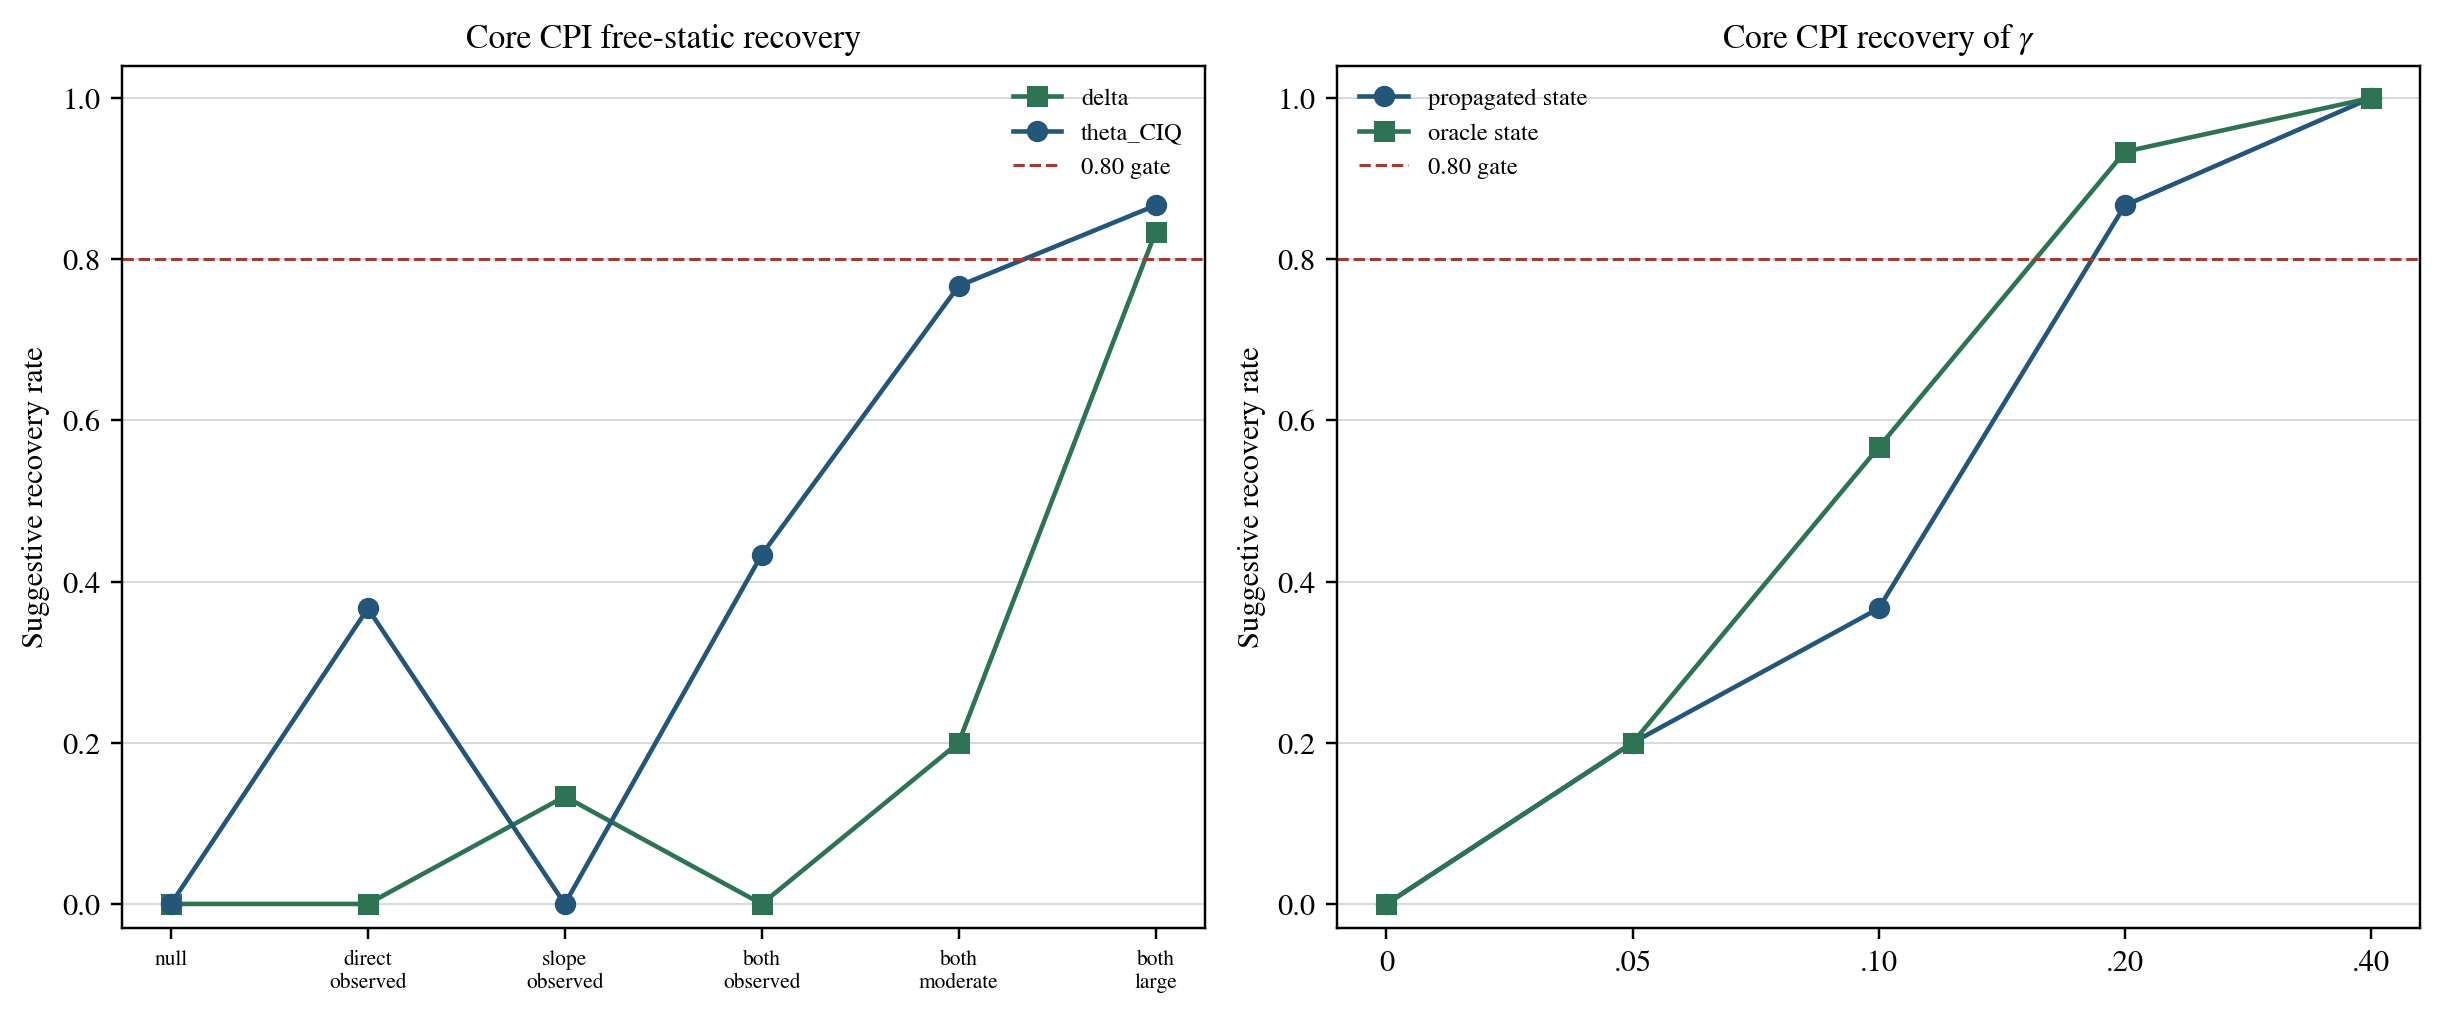
\includegraphics[width=0.93\linewidth]{core_recovery.png}
\caption{Core CPI free-static and varying-theta recovery.}
\end{figure}

The recovery sampler passes comfortably: maximum R-hat is 1.0207 and minimum bulk ESS is
331.9. The observed-scale effects fail because they are detected too infrequently, not
because recovery chains fail to mix.

% -----------------------------------------------------------------------------
\section{Core CPI Implied Paths and In-Sample Fit}

\begin{figure}[H]
\centering
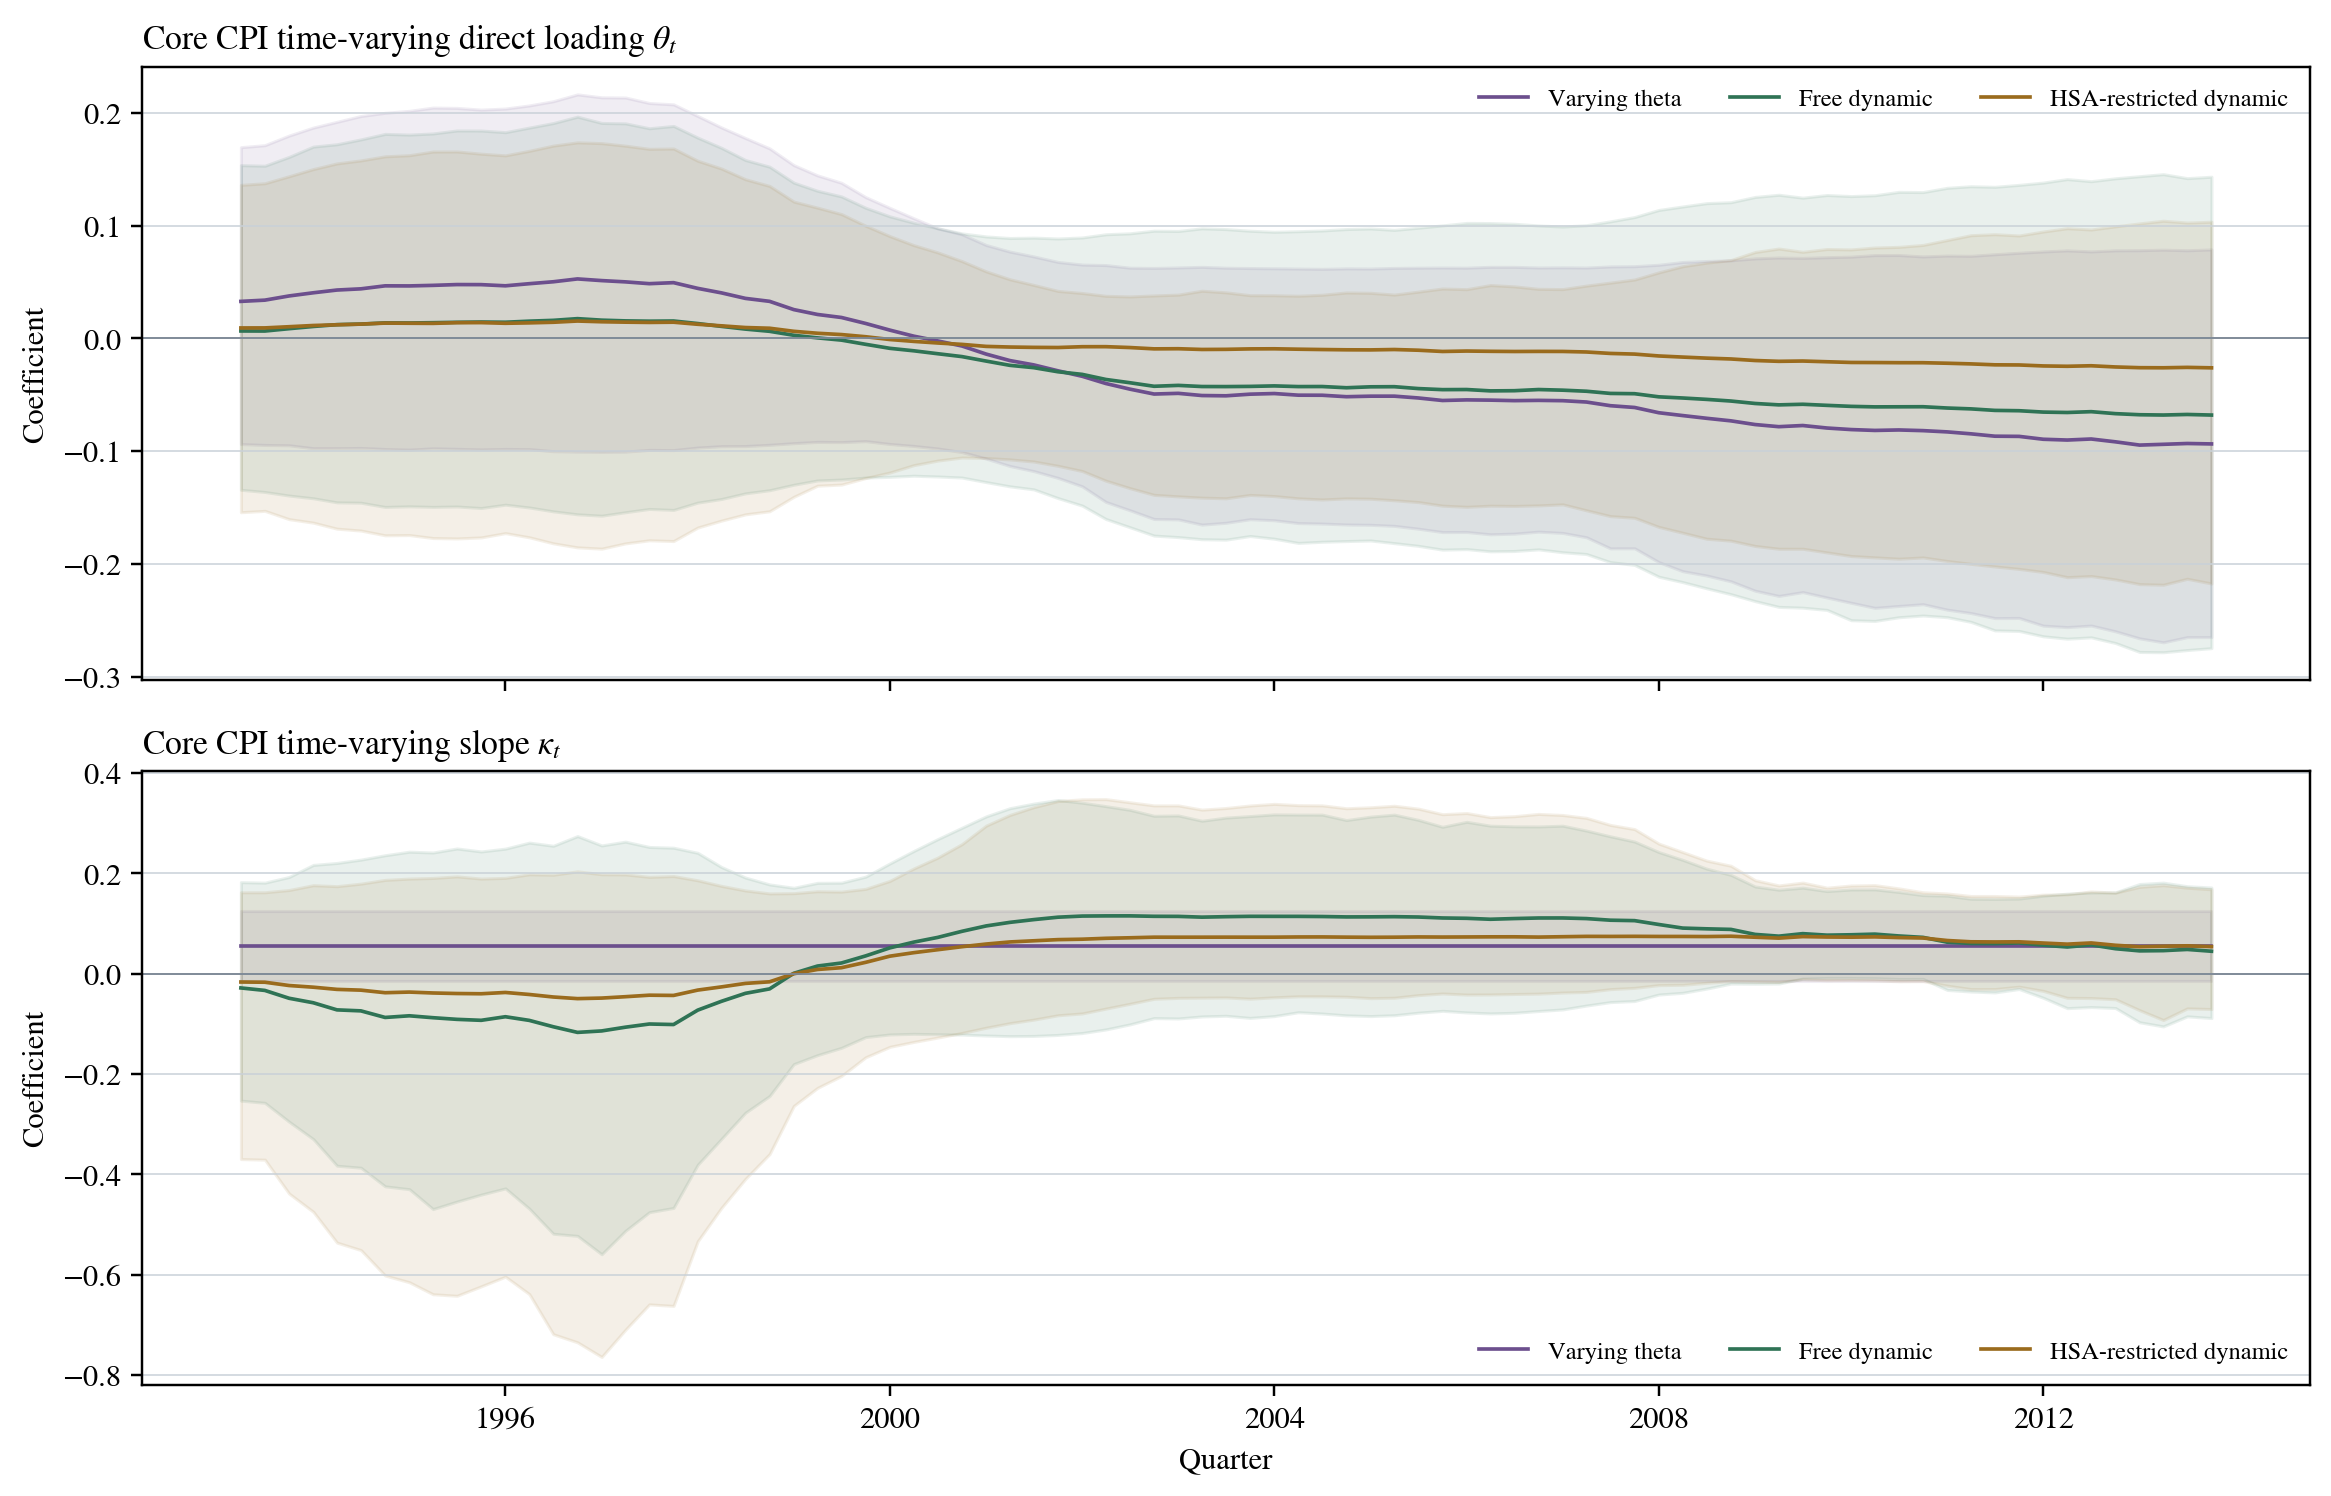
\includegraphics[width=0.94\linewidth]{core_dynamic_paths.png}
\caption{Core CPI implied $\theta_t$ and $\kappa_t$ paths in the firm-weighted unemployment-gap cell.}
\end{figure}

The positive median drift in $\theta_t$ is generated by a positive but zero-crossing $\gamma$
multiplied by the smooth slow state. The pointwise bands overlap zero over the sample. As for
PPI, motion in the posterior median is not equivalent to identification of historical
time variation.

\begin{figure}[H]
\centering
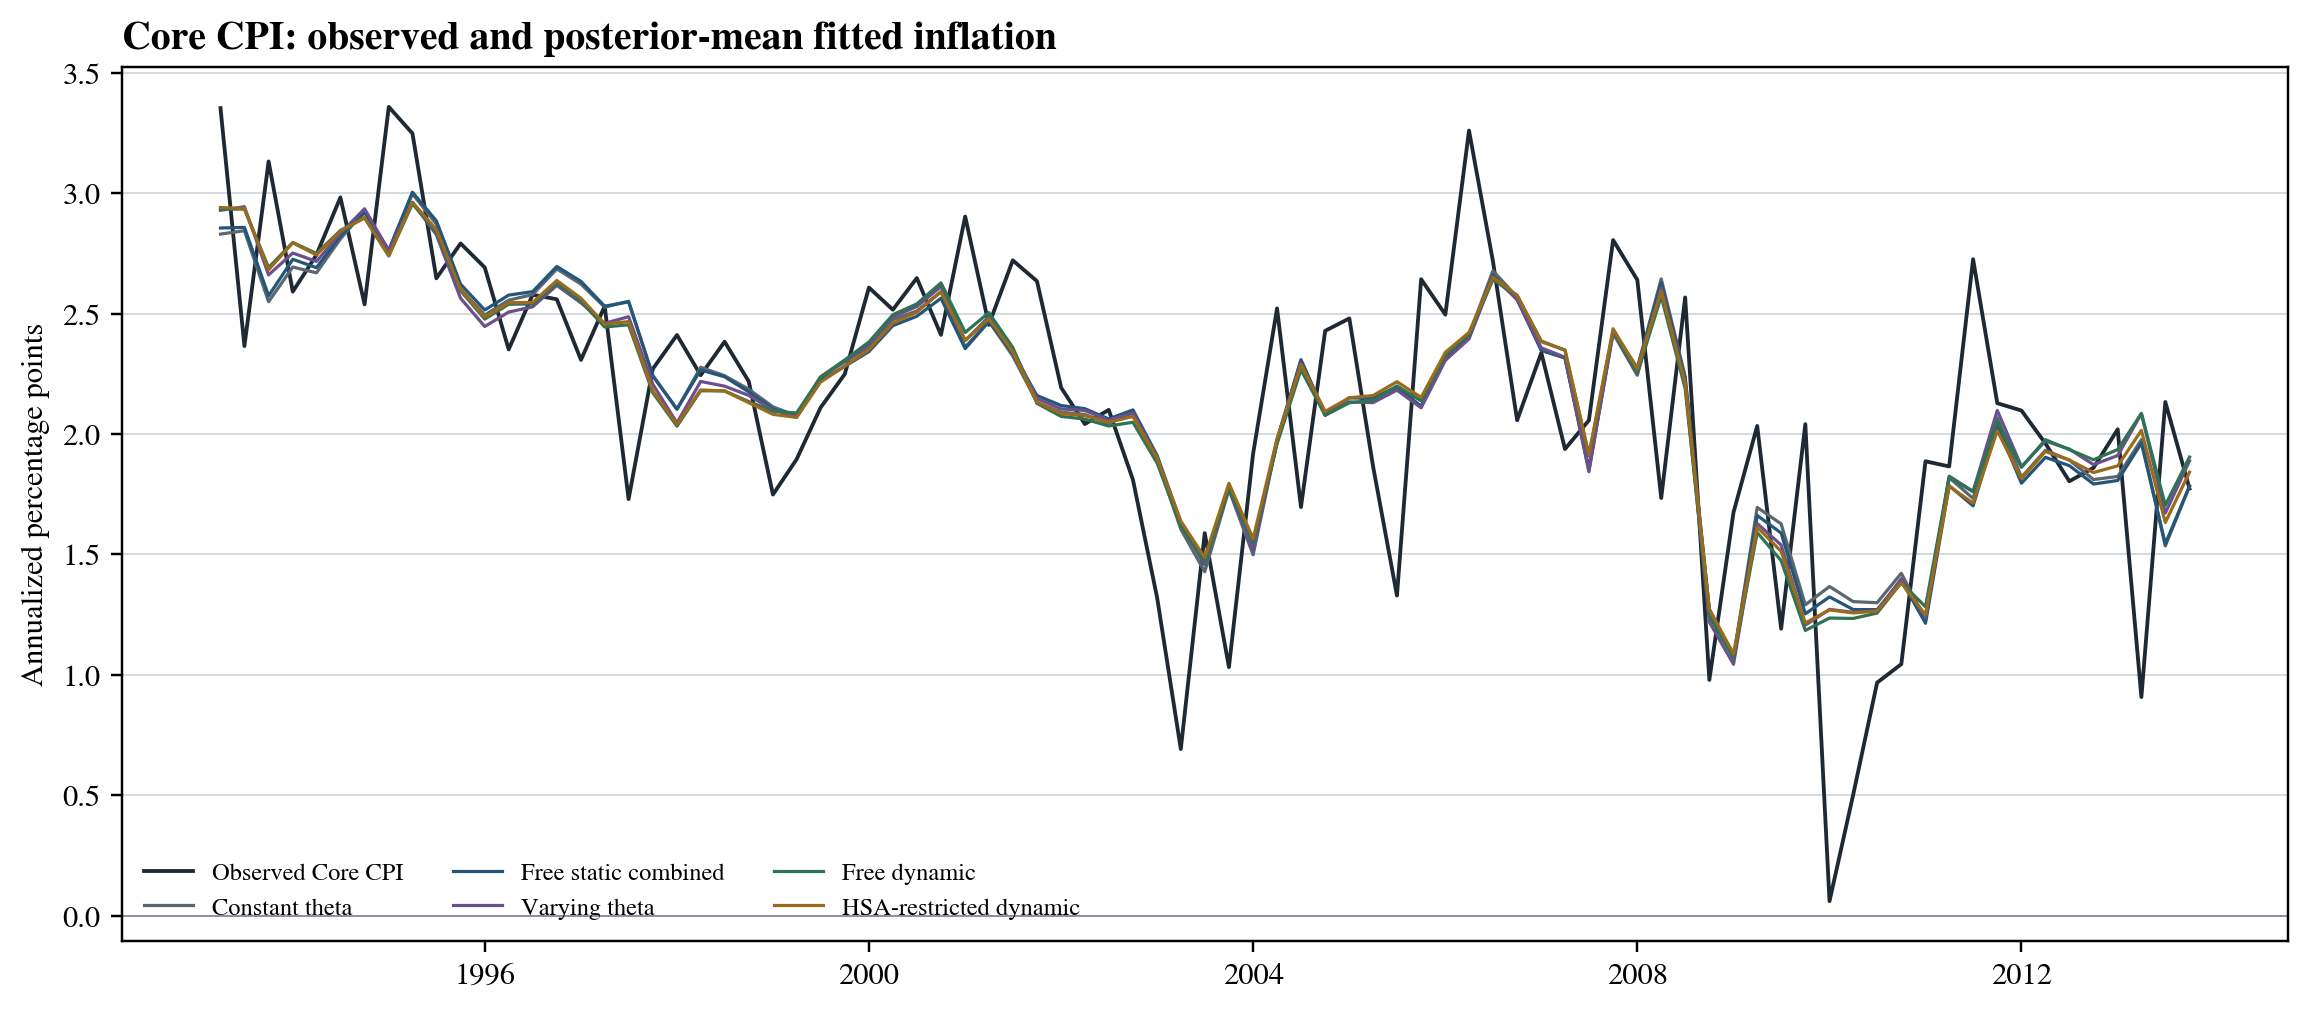
\includegraphics[width=0.92\linewidth]{core_posterior_fit.png}
\caption{Observed Core CPI and posterior-mean fitted values.}
\end{figure}

The five fitted means are close. The extra competition interactions alter a small component
of fitted Core CPI rather than accounting for a visibly distinct inflation movement.

% -----------------------------------------------------------------------------
\section{Core CPI Prediction, AR(1) Robustness, and Convergence}

\begin{table}[H]
\centering
\caption{Core CPI M1--M4 relative to M0 constant theta}
\resizebox{\linewidth}{!}{\begin{tabular}{@{}lllrrrrr@{}}
\toprule
Cycle & Activity & Model & $\Delta$LOO & $\Delta$WAIC & $\Delta$holdout & $\Delta$RMSE & max $k$ \\
\midrule
firm\_weighted & inverse\_markup & Free static combined & -0.436 & -0.459 & 0.124 & -0.001 & 0.46 \\
firm\_weighted & inverse\_markup & Varying theta & -0.240 & -0.217 & -0.443 & 0.017 & 0.51 \\
firm\_weighted & inverse\_markup & Free dynamic & -1.046 & -0.954 & -0.092 & 0.009 & 0.55 \\
firm\_weighted & inverse\_markup & HSA-restricted dynamic & -0.459 & -0.415 & 0.036 & 0.006 & 0.47 \\
firm\_weighted & negative\_unemployment\_gap & Free static combined & -0.105 & -0.133 & 0.321 & -0.000 & 0.43 \\
firm\_weighted & negative\_unemployment\_gap & Varying theta & 0.004 & 0.068 & 0.005 & 0.007 & 0.50 \\
firm\_weighted & negative\_unemployment\_gap & Free dynamic & -0.447 & -0.315 & -3.118 & 0.103 & 0.64 \\
firm\_weighted & negative\_unemployment\_gap & HSA-restricted dynamic & -0.236 & -0.146 & -2.348 & 0.079 & 0.44 \\
revenue\_weighted & inverse\_markup & Free static combined & -0.268 & -0.244 & -0.037 & 0.002 & 0.46 \\
revenue\_weighted & inverse\_markup & Varying theta & -0.563 & -0.443 & -0.769 & 0.024 & 0.55 \\
revenue\_weighted & inverse\_markup & Free dynamic & -1.215 & -1.095 & -0.301 & 0.009 & 0.69 \\
revenue\_weighted & inverse\_markup & HSA-restricted dynamic & -0.542 & -0.480 & -0.137 & 0.008 & 0.54 \\
revenue\_weighted & negative\_unemployment\_gap & Free static combined & -0.064 & -0.060 & 0.309 & -0.000 & 0.55 \\
revenue\_weighted & negative\_unemployment\_gap & Varying theta & -0.374 & -0.299 & -0.076 & 0.009 & 0.65 \\
revenue\_weighted & negative\_unemployment\_gap & Free dynamic & -0.740 & -0.599 & -3.326 & 0.110 & 0.56 \\
revenue\_weighted & negative\_unemployment\_gap & HSA-restricted dynamic & -0.433 & -0.335 & -2.211 & 0.078 & 0.57 \\
\bottomrule
\end{tabular}
}
\end{table}

Free static improves holdout ELPD slightly in three of four cells, by at most 0.321, while
its LOO and WAIC differences are negative. The isolated M2 improvement is essentially zero
in the firm-weighted unemployment-gap cell. M3 and M4 produce sizable holdout losses in both
unemployment-gap cells. No extension therefore improves prediction consistently across
cycle definitions, activities, and scoring rules. Core-CPI Pareto values are below 0.7, so
its LOO calculation is more stable than the PPI comparison, but it still favors parsimony.

\begin{figure}[H]
\centering
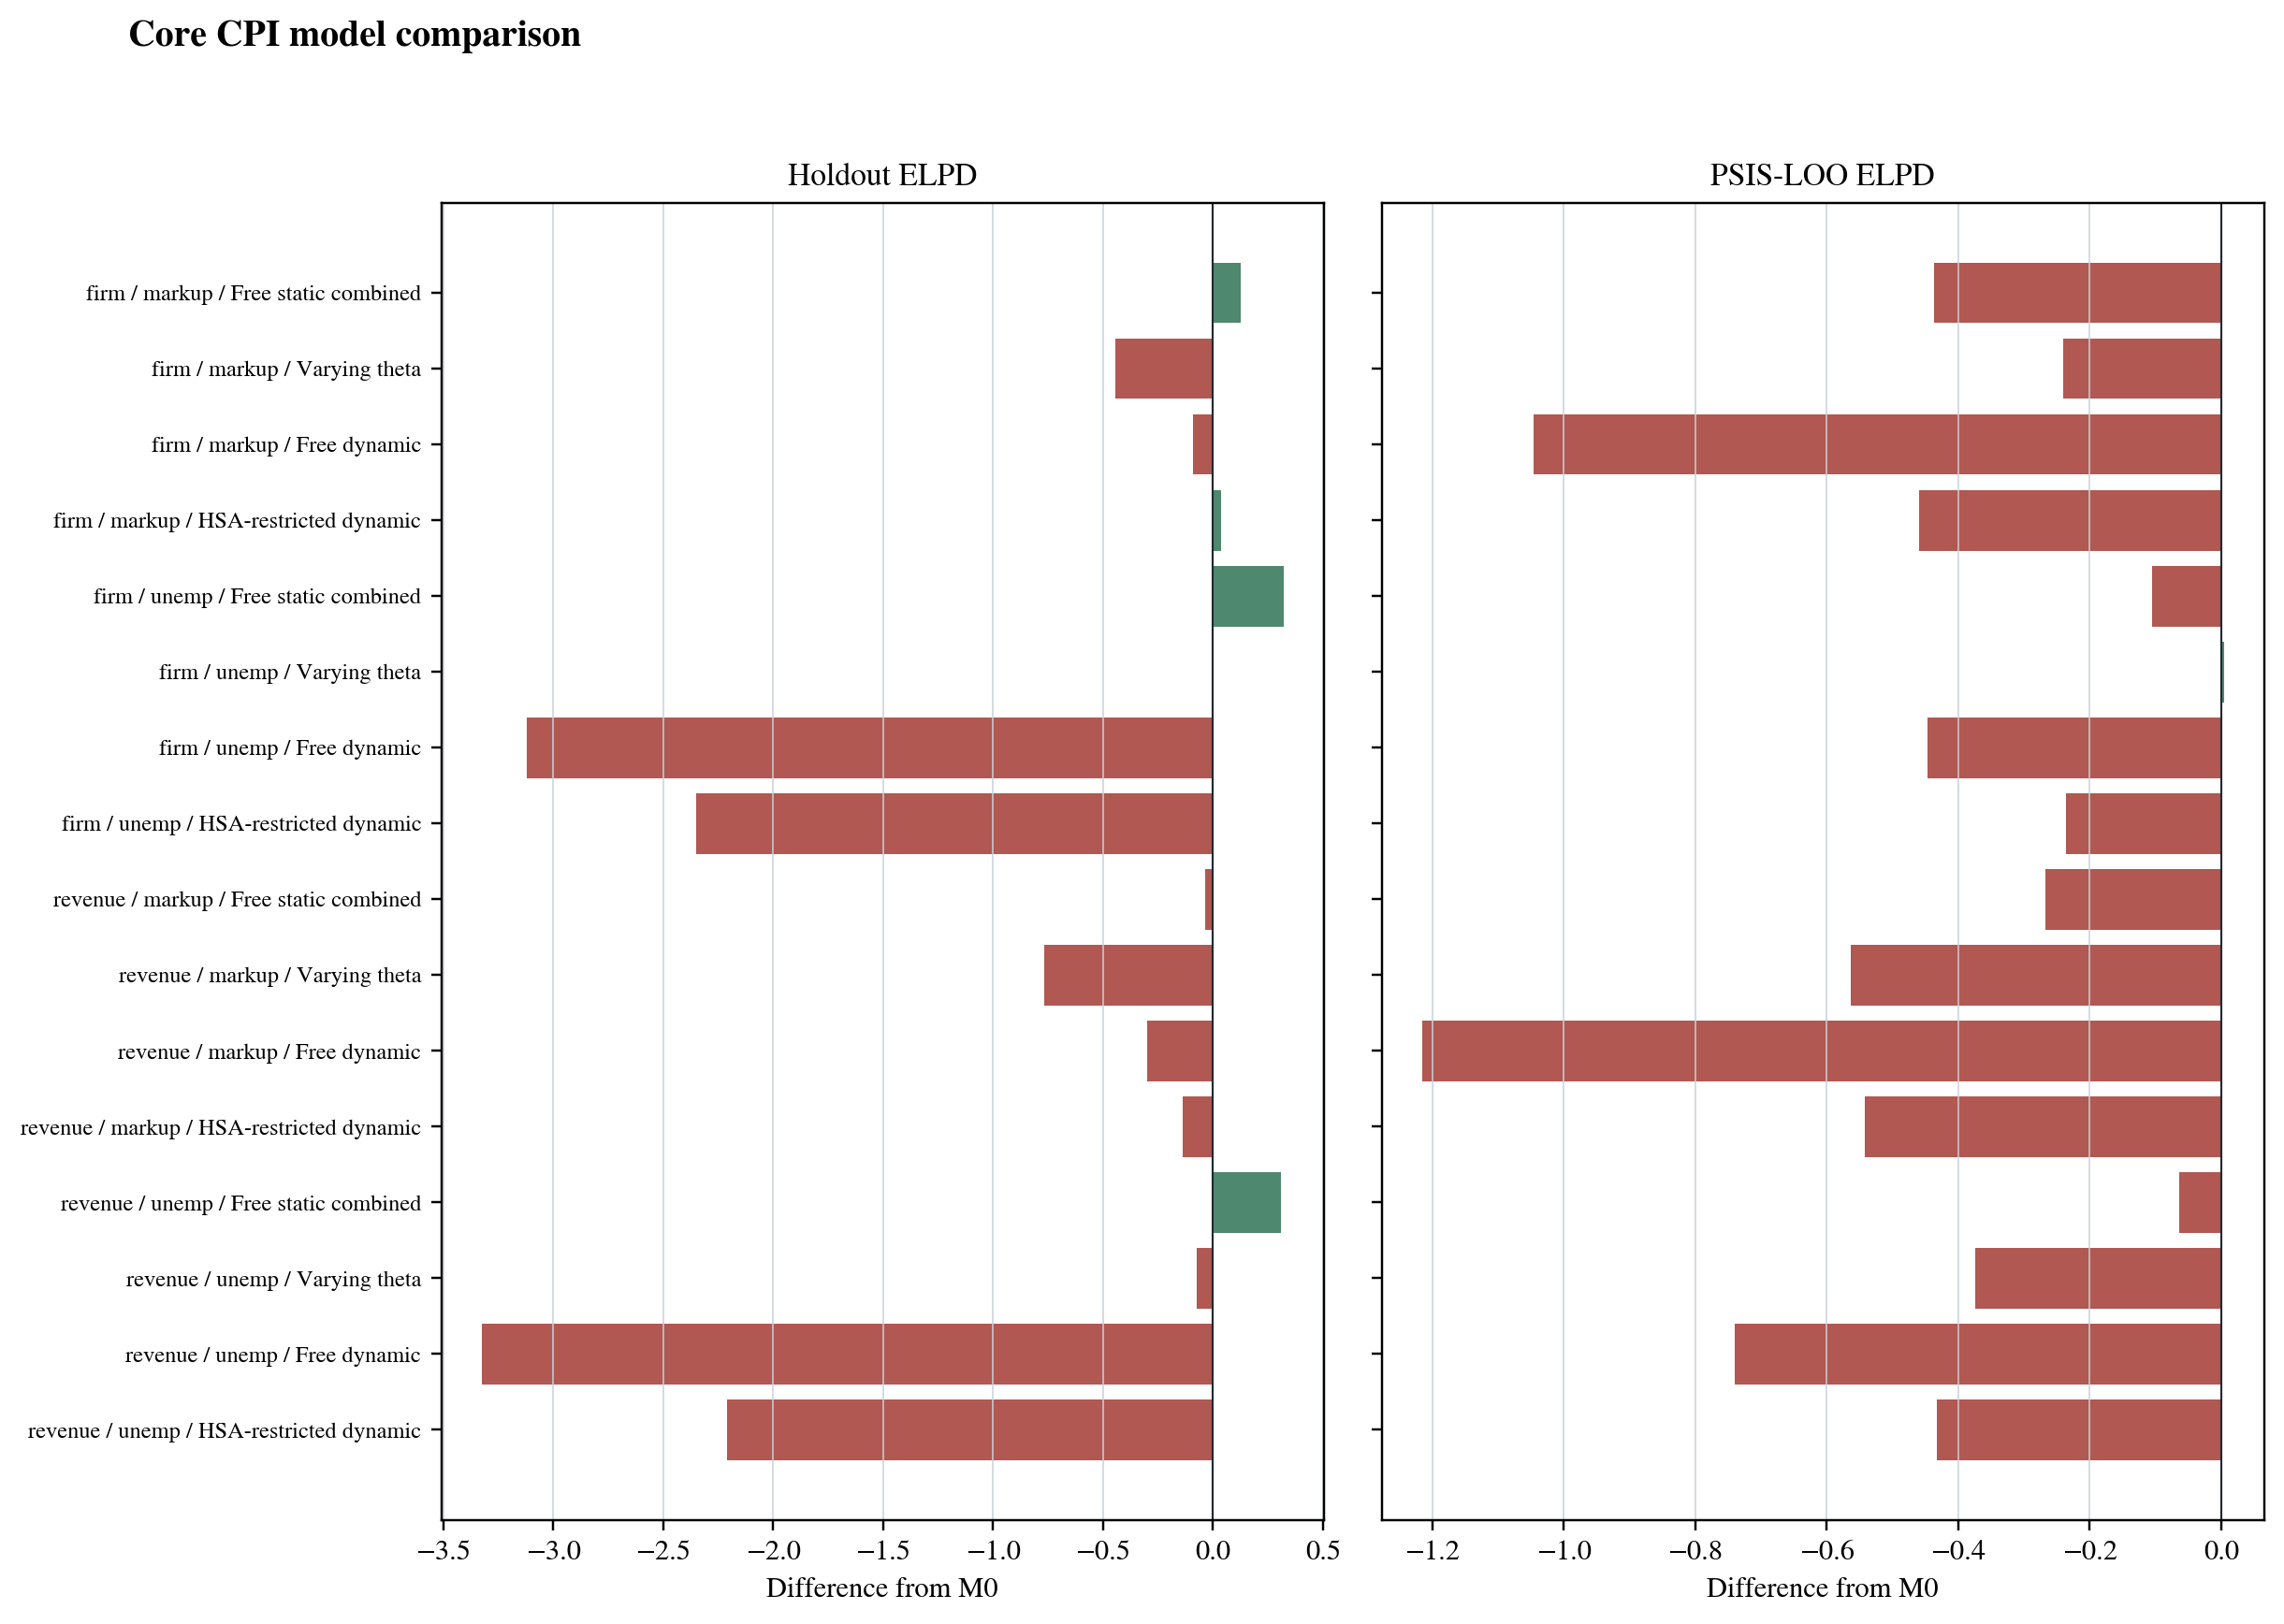
\includegraphics[width=0.91\linewidth]{core_model_comparison.png}
\caption{Core CPI predictive comparison relative to M0.}
\end{figure}

\begin{table}[H]
\centering
\caption{Core CPI IID versus persistent AR(1), firm-weighted unemployment-gap cell}
\scriptsize
\begin{tabular}{@{}llcc@{}}
\toprule
Model & Parameter & IID & Persistent AR(1) \\
\midrule
Constant theta & theta\_CIQ & \makecell{-0.016\\{\scriptsize [-0.111, 0.078]}} & \makecell{-0.021\\{\scriptsize [-0.106, 0.064]}} \\
Free static combined & delta & \makecell{-0.016\\{\scriptsize [-0.067, 0.037]}} & \makecell{-0.009\\{\scriptsize [-0.063, 0.041]}} \\
Free static combined & theta\_CIQ & \makecell{-0.029\\{\scriptsize [-0.133, 0.072]}} & \makecell{-0.027\\{\scriptsize [-0.126, 0.067]}} \\
Varying theta & theta\_0 & \makecell{-0.026\\{\scriptsize [-0.121, 0.069]}} & \makecell{-0.029\\{\scriptsize [-0.116, 0.060]}} \\
Varying theta & gamma & \makecell{0.030\\{\scriptsize [-0.025, 0.087]}} & \makecell{0.027\\{\scriptsize [-0.023, 0.079]}} \\
Free dynamic & delta\_1 & \makecell{-0.023\\{\scriptsize [-0.081, 0.034]}} & \makecell{-0.018\\{\scriptsize [-0.075, 0.039]}} \\
Free dynamic & delta\_2 & \makecell{-0.024\\{\scriptsize [-0.097, 0.048]}} & \makecell{-0.022\\{\scriptsize [-0.090, 0.050]}} \\
Free dynamic & theta\_0 & \makecell{-0.028\\{\scriptsize [-0.138, 0.088]}} & \makecell{-0.028\\{\scriptsize [-0.134, 0.077]}} \\
Free dynamic & gamma & \makecell{0.018\\{\scriptsize [-0.048, 0.083]}} & \makecell{0.016\\{\scriptsize [-0.046, 0.082]}} \\
HSA-restricted dynamic & theta\_0 & \makecell{-0.016\\{\scriptsize [-0.111, 0.044]}} & \makecell{-0.014\\{\scriptsize [-0.103, 0.046]}} \\
HSA-restricted dynamic & gamma & \makecell{0.009\\{\scriptsize [-0.057, 0.071]}} & \makecell{0.009\\{\scriptsize [-0.051, 0.064]}} \\
HSA-restricted dynamic & lambda & \makecell{0.564\\{\scriptsize [-8.287, 9.120]}} & \makecell{0.524\\{\scriptsize [-7.949, 9.008]}} \\
\bottomrule
\end{tabular}

\end{table}

AR(1) errors do not restore the HSA signs. The complete observed Core-CPI run has maximum
R-hat 1.0036 and minimum bulk ESS 1,220.2.

\begin{table}[H]
\centering
\caption{Core CPI observed IID convergence}
\scriptsize
\begin{tabular}{@{}llrr@{}}
\toprule
Model & Cell & Max R-hat & Min bulk ESS \\
\midrule
Constant theta & Firm / unemployment & 1.0013 & 2506.3 \\
Constant theta & Revenue / unemployment & 1.0013 & 2565.3 \\
Constant theta & Firm / inverse markup & 1.0002 & 2496.8 \\
Constant theta & Revenue / inverse markup & 1.0008 & 2720.7 \\
Free static combined & Firm / unemployment & 1.0015 & 2272.7 \\
Free static combined & Revenue / unemployment & 1.0009 & 2722.5 \\
Free static combined & Firm / inverse markup & 1.0027 & 2534.3 \\
Free static combined & Revenue / inverse markup & 1.0011 & 2486.9 \\
Varying theta & Firm / unemployment & 1.0006 & 6664.0 \\
Varying theta & Revenue / unemployment & 1.0007 & 6284.3 \\
Varying theta & Firm / inverse markup & 1.0005 & 6442.0 \\
Varying theta & Revenue / inverse markup & 1.0006 & 6538.9 \\
Free dynamic & Firm / unemployment & 1.0008 & 6788.1 \\
Free dynamic & Revenue / unemployment & 1.0010 & 6648.0 \\
Free dynamic & Firm / inverse markup & 1.0012 & 6200.0 \\
Free dynamic & Revenue / inverse markup & 1.0012 & 6388.3 \\
HSA-restricted dynamic & Firm / unemployment & 1.0016 & 1413.2 \\
HSA-restricted dynamic & Revenue / unemployment & 1.0021 & 1639.9 \\
HSA-restricted dynamic & Firm / inverse markup & 1.0003 & 3825.2 \\
HSA-restricted dynamic & Revenue / inverse markup & 1.0004 & 3951.1 \\
\bottomrule
\end{tabular}

\end{table}

The computational conclusion is unambiguous: the Core-CPI sign differences and wide HSA
intervals are posterior features, not nonconvergence artifacts.

% -----------------------------------------------------------------------------
\section{Prespecified Oil-Control Extension}

\subsection{Why this is an admissible robustness exercise}

QoQ PPI contains a large input-cost component, especially around the 2008--09 oil-price
collapse and rebound. If that component is omitted, it can inflate the NKPC residual variance
and reduce precision. It can also bias a competition coefficient if oil-price changes happen
to covary with the competition regressors. The extension was therefore fixed before it was
run: one oil series, one transformation, and exactly the current and first lag. No result-based
lag selection or sign restriction was allowed.

Let $R_t^o$ denote the repository's FRED-derived real WTI-to-CPI index and define
\begin{equation}
q_t^o=400\left(\log R_t^o-\log R_{t-1}^o\right).
\label{eq:oil}
\end{equation}
The normalization of the level cancels in the log difference. Every M0--M4 equation is
augmented in exactly the same way:
\begin{align}
\pi_t^q={}&a+\alpha_b\pi_{t-1}^q+\alpha_fE_t\pi_{t+1}^q
+\beta_{o,0}q_t^o+\beta_{o,1}q_{t-1}^o \notag\\
&+\kappa_t x_t-\theta_t\Nhat_t+\varepsilon_t.
\label{eq:oil_nkpc}
\end{align}
The definitions of $\kappa_t$ and $\theta_t$ remain those of M0--M4 in Section~7. Thus oil
is a conditional input-cost control, not an additional competition channel, and the
competition-state posterior remains cut from inflation.

The oil priors are zero-mean Gaussian. For $j\in\{0,1\}$,
\begin{equation}
\beta_{o,j}\sim N\!\left(0,\left[\frac{s_\pi}{s_{q_j^o}}\right]^2\right).
\end{equation}
This gives the effect of a one-SD oil movement a prior SD of one outcome SD. The prior is
weak relative to the observed PPI pass-through and is applied by the same scale rule to Core
CPI.

\begin{table}[H]
\centering
\caption{Oil-control data summary}
\begin{tabular}{@{}p{0.15\linewidth}p{0.25\linewidth}p{0.16\linewidth}cccrr@{}}
\toprule
Series & Source & Transformation & Start & End & $T$ & Mean & SD \\
\midrule
Oil control & FRED-derived real WTI/CPI index & $400\Delta\log R_t^o$ & 1993Q2 & 2013Q4 & 83 & 5.295 & 54.921 \\
Oil control, lag 1 & Same series & $q_{t-1}^o$ & 1993Q2 & 2013Q4 & 83 & 5.523 & 54.791 \\
\bottomrule
\end{tabular}

\end{table}

Two cautions remain. First, the input is a real WTI/CPI index, so the CPI denominator makes
it a relative input-price control rather than a pure nominal oil shock. Second, current oil
prices are not instrumented and may respond to aggregate conditions. The coefficient is
therefore conditional pass-through, not a causal oil-shock estimate.

\begin{figure}[H]
\centering
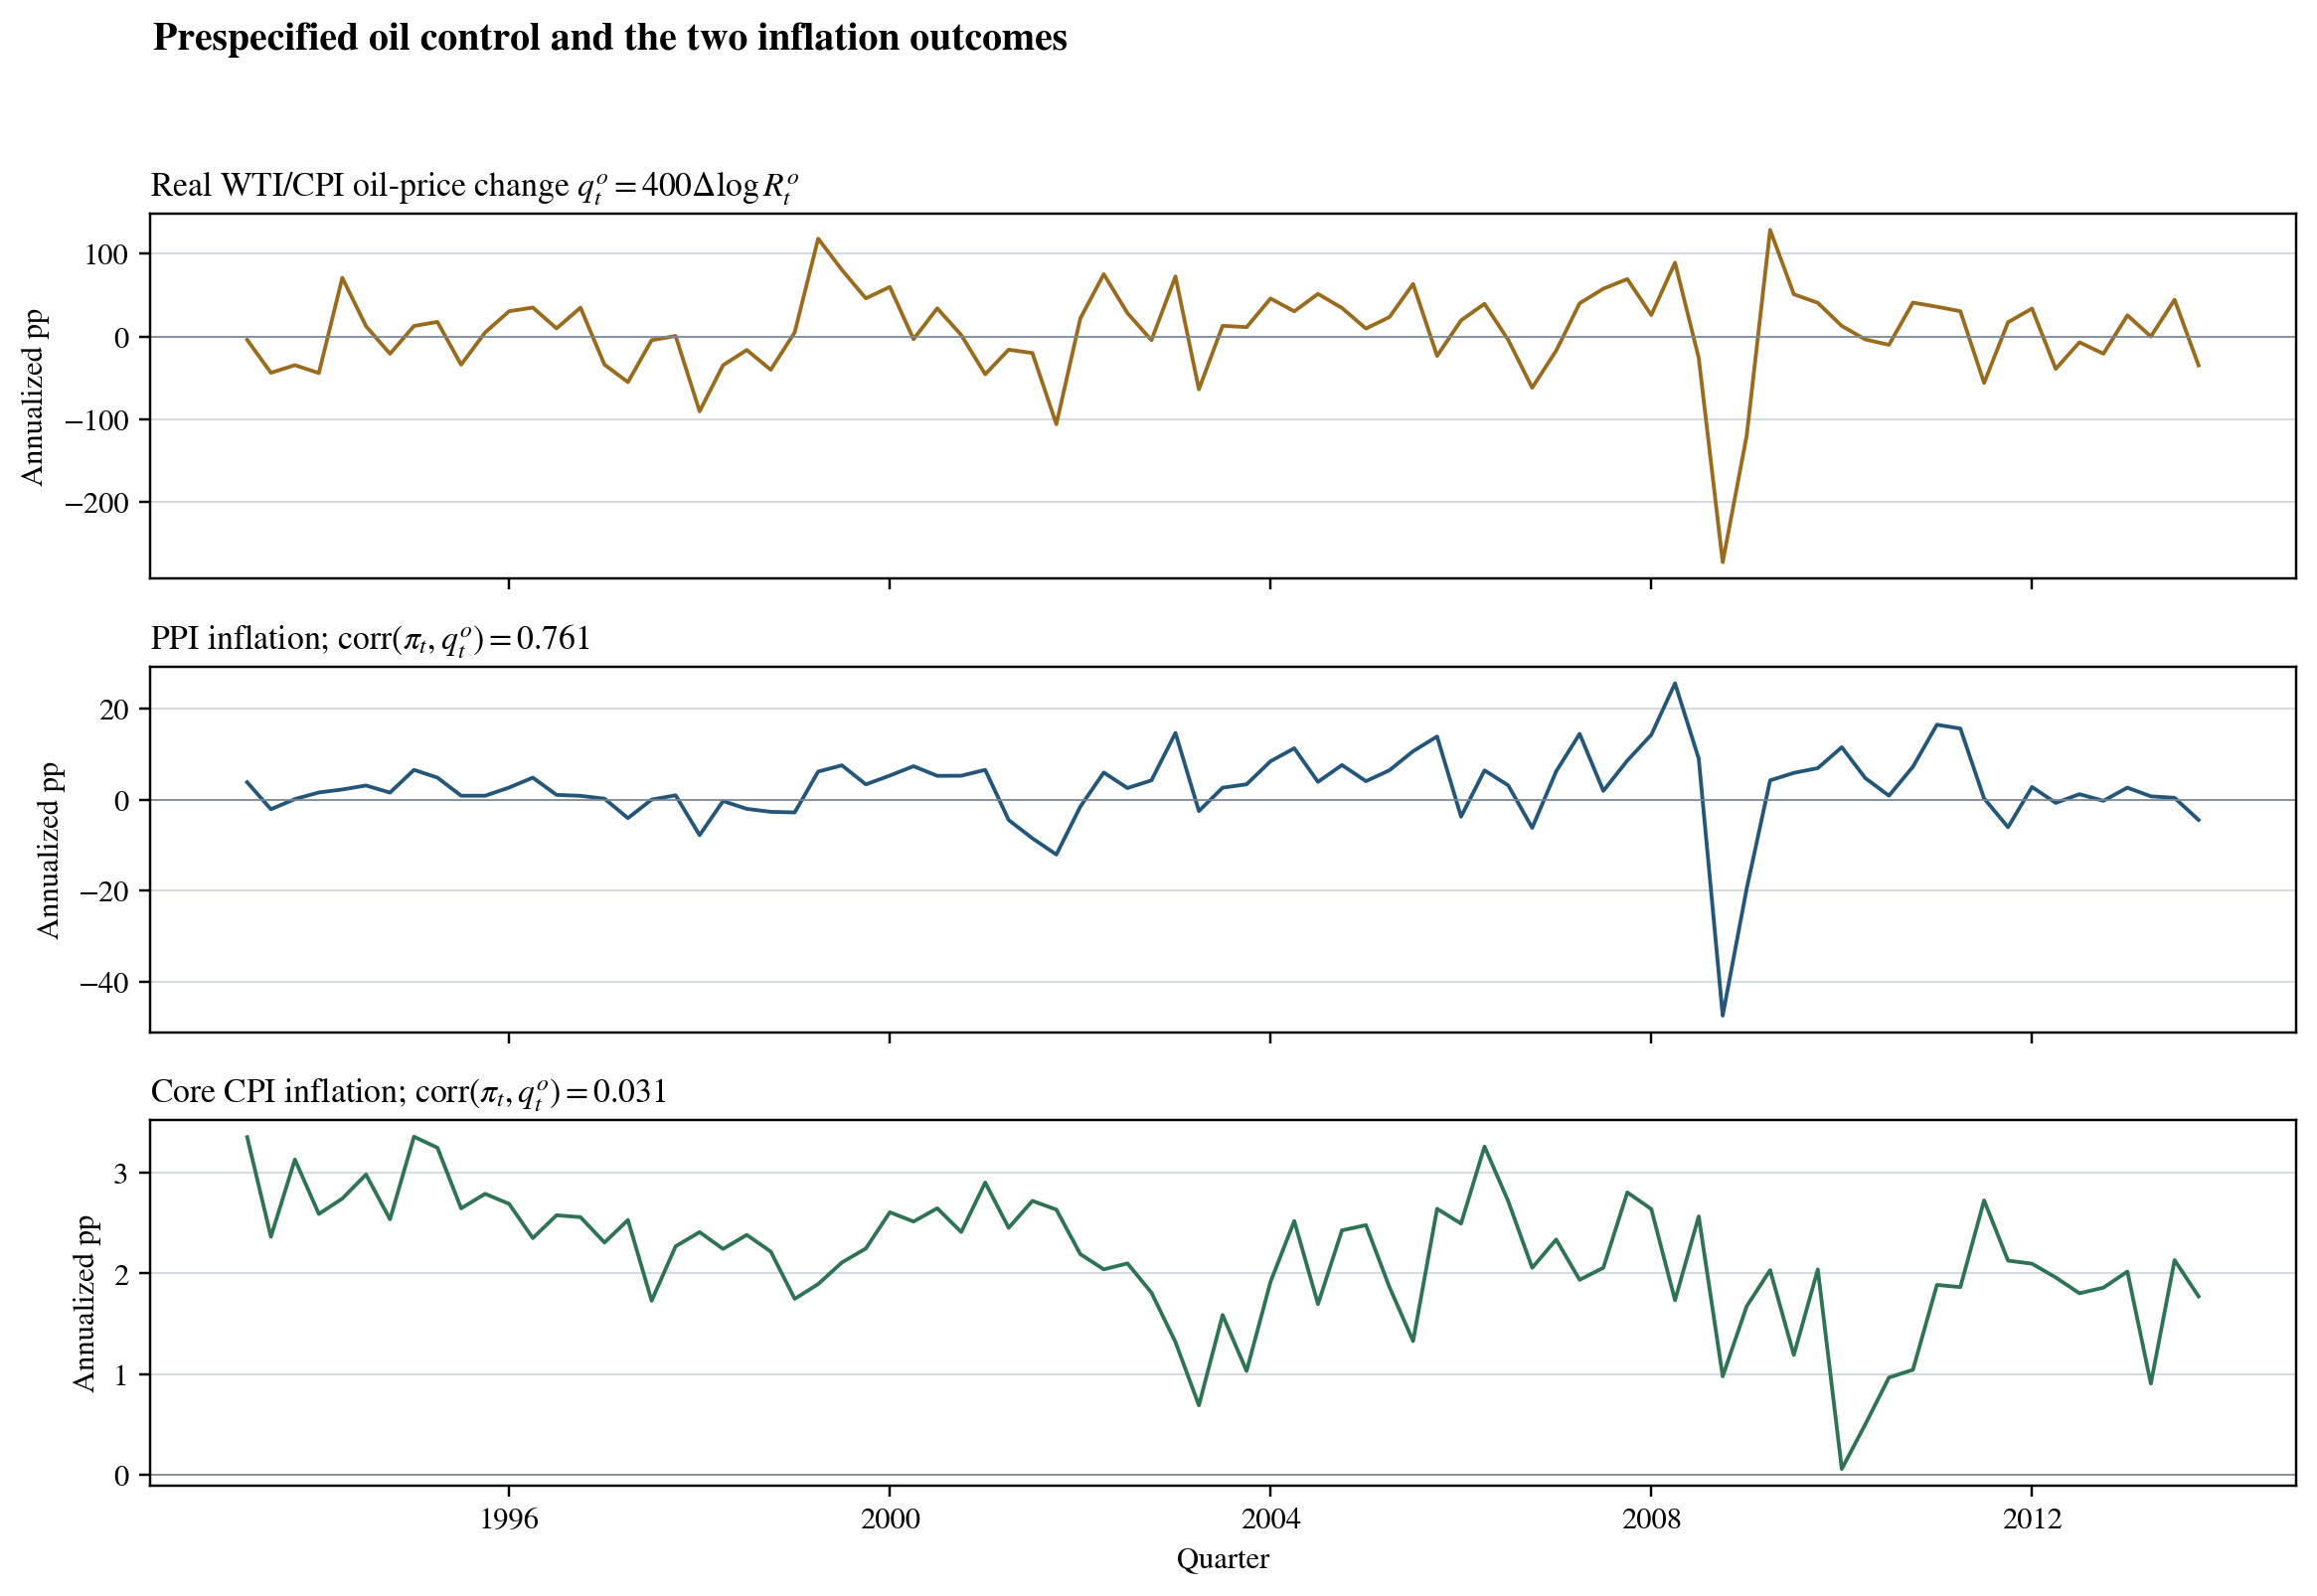
\includegraphics[width=0.90\linewidth]{oil_timeseries.png}
\caption{Prespecified real-oil-price control and the matched inflation outcomes.}
\end{figure}

The sample correlation of current oil-price change with PPI inflation is 0.761, compared
with 0.031 for Core CPI. More importantly for omitted-variable bias, its correlations with
the firm-weighted posterior-mean Capital-IQ cycle, the Gustavo slow state, and the negative
unemployment gap are only $-0.040$, $-0.059$, and 0.019. The oil extension therefore mostly
removes PPI residual variation rather than projecting out the competition regressors.

% -----------------------------------------------------------------------------
\section{Oil-Control Coefficients and Competition-Channel Stability}

\begin{figure}[H]
\centering
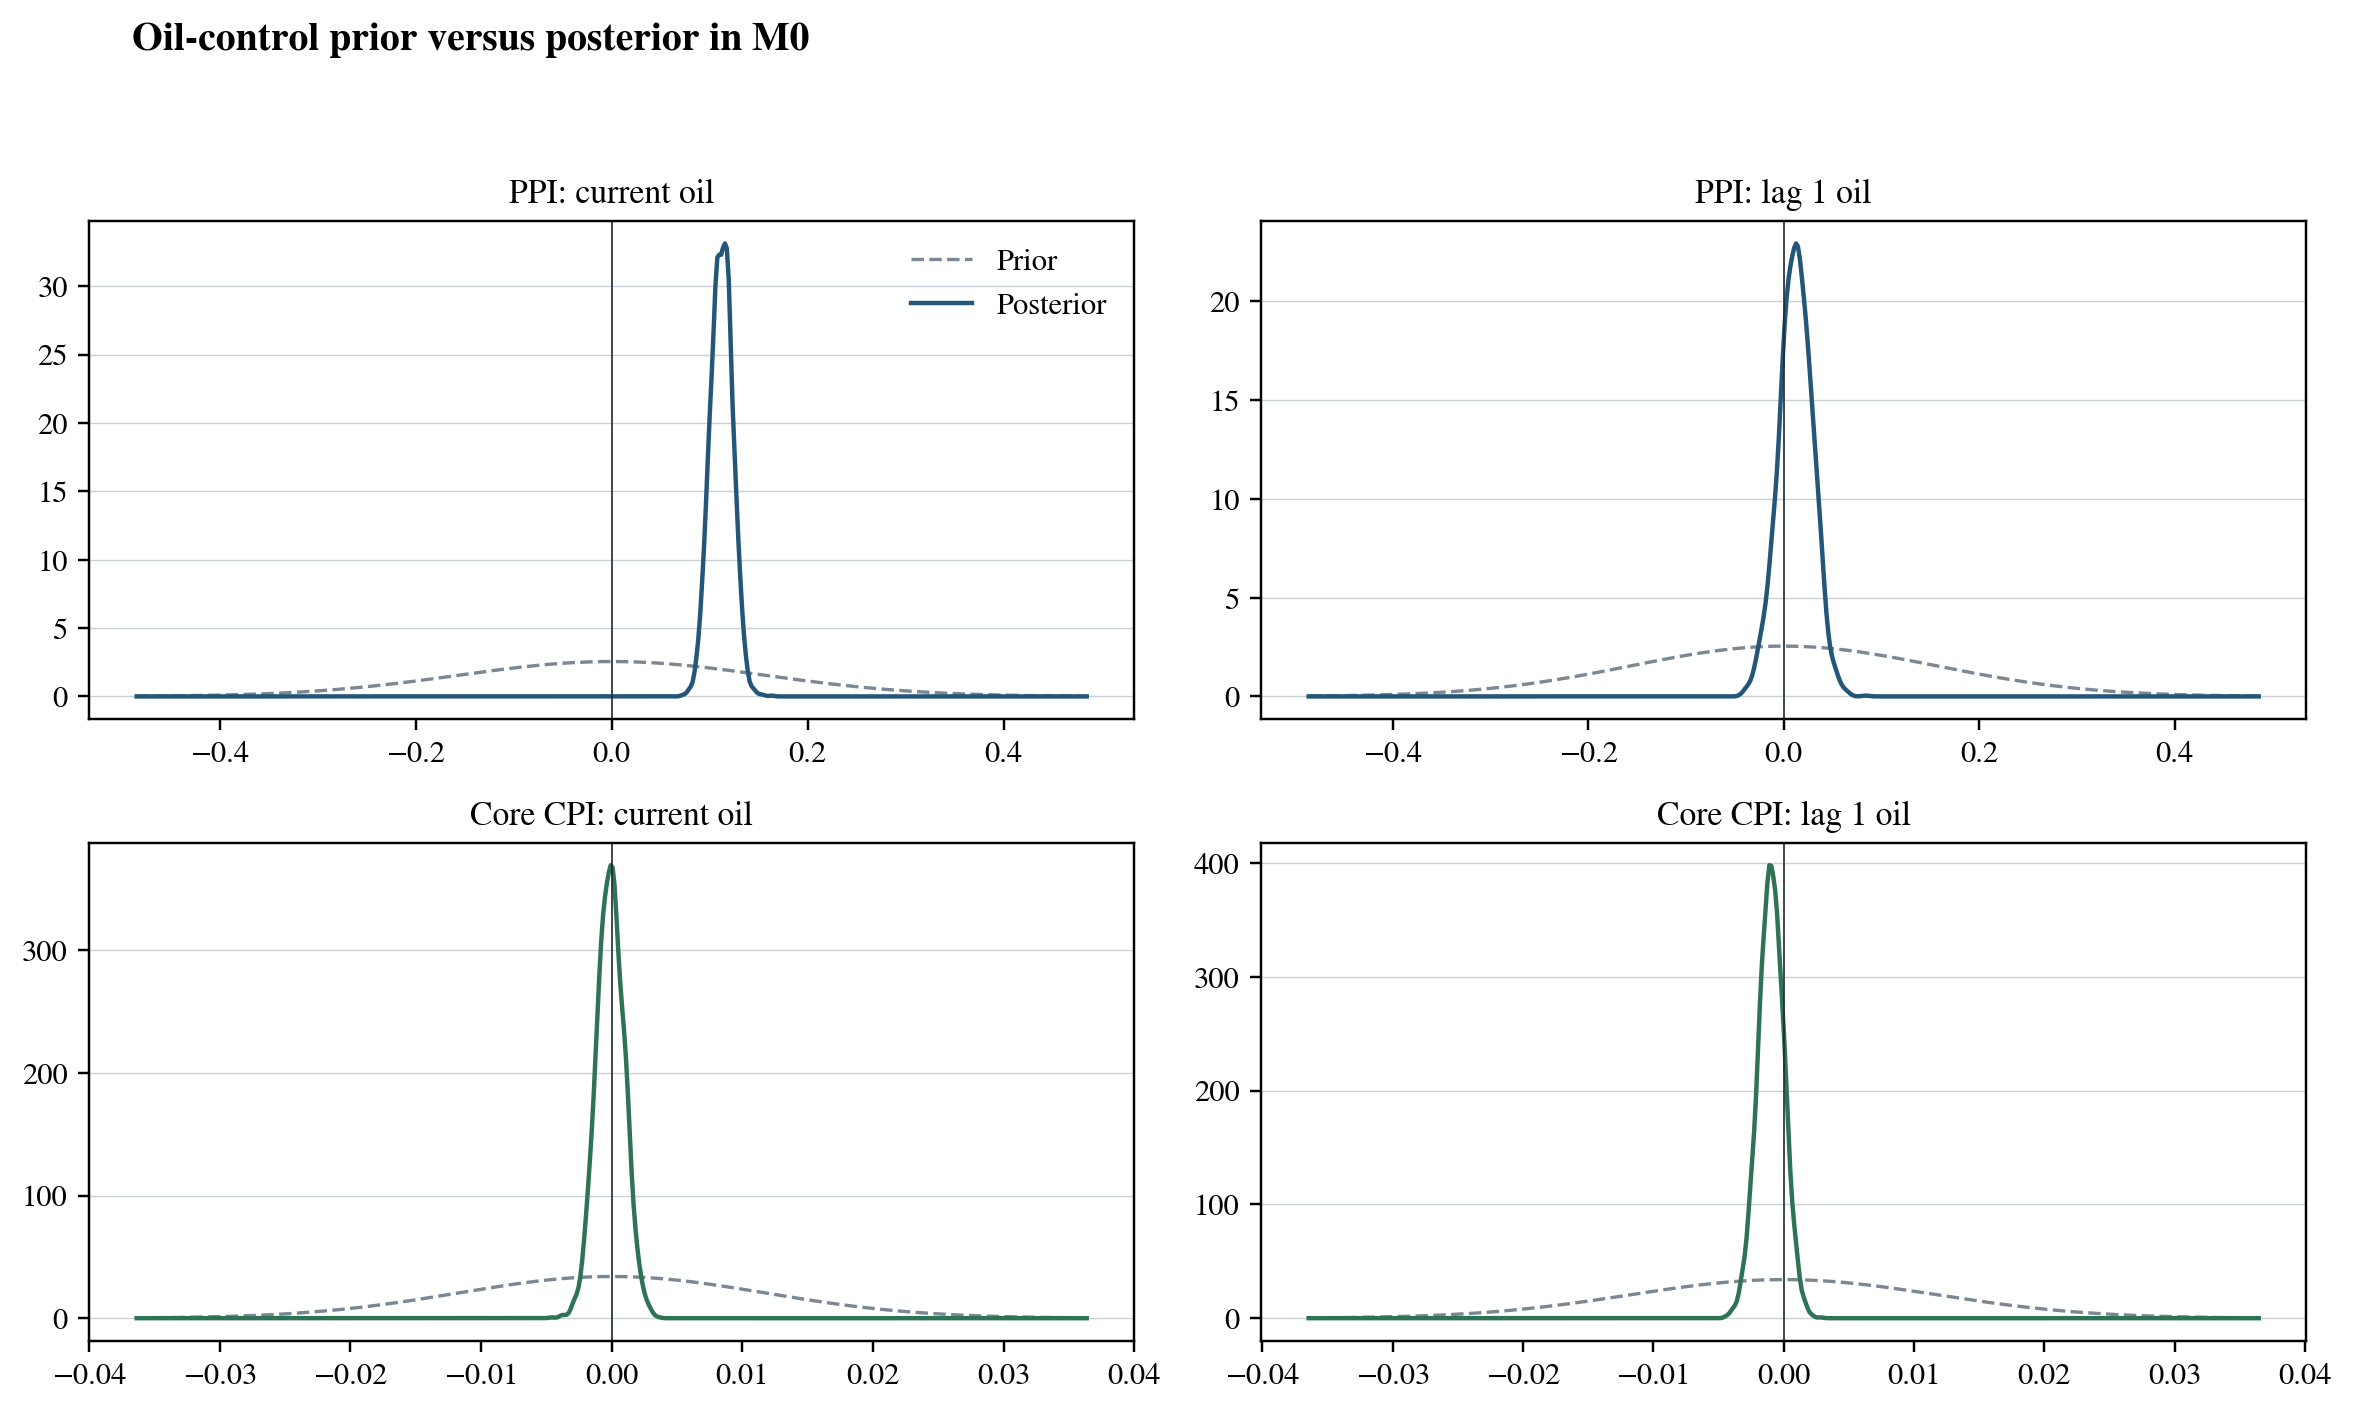
\includegraphics[width=0.88\linewidth]{oil_prior_posterior.png}
\caption{Prior versus posterior for current and lagged oil controls in M0.}
\end{figure}

For PPI the current coefficient is exceptionally well learned:
\[
\beta_{o,0}=0.112[0.091,0.133],\qquad
\beta_{o,1}=0.012[-0.023,0.045]
\]
in the firm-weighted unemployment-gap M0 cell. The lag-one coefficient is directionally
positive but not separately sign-identified. For Core CPI both coefficients are economically
near zero. This outcome difference is visible in the posterior densities and is not imposed
by their priors.

\begin{table}[H]
\centering
\caption{Oil-control coefficients and competition targets; firm-weighted cells}
\scriptsize
\begin{tabular}{@{}lcccc@{}}
\toprule
Target & PPI / unemployment & PPI / inverse markup & Core CPI / unemployment & Core CPI / inverse markup \\
\midrule
M0 $\beta_{o,0}$ & \makecell{0.112\\{\scriptsize [0.091, 0.133]}} & \makecell{0.111\\{\scriptsize [0.089, 0.133]}} & \makecell{-0.000\\{\scriptsize [-0.002, 0.002]}} & \makecell{-0.000\\{\scriptsize [-0.002, 0.002]}} \\
M0 $\beta_{o,1}$ & \makecell{0.012\\{\scriptsize [-0.023, 0.045]}} & \makecell{0.012\\{\scriptsize [-0.022, 0.045]}} & \makecell{-0.001\\{\scriptsize [-0.003, 0.001]}} & \makecell{-0.001\\{\scriptsize [-0.003, 0.001]}} \\
M0 $\theta$ & \makecell{0.691\\{\scriptsize [-0.391, 1.813]}} & \makecell{0.723\\{\scriptsize [-0.310, 1.782]}} & \makecell{-0.015\\{\scriptsize [-0.115, 0.078]}} & \makecell{-0.022\\{\scriptsize [-0.123, 0.070]}} \\
M1 $\delta$ & \makecell{0.072\\{\scriptsize [-0.538, 0.710]}} & \makecell{0.042\\{\scriptsize [-2.384, 2.421]}} & \makecell{-0.013\\{\scriptsize [-0.068, 0.039]}} & \makecell{0.029\\{\scriptsize [-0.213, 0.266]}} \\
M1 $\theta$ & \makecell{0.775\\{\scriptsize [-0.443, 2.016]}} & \makecell{0.732\\{\scriptsize [-0.374, 1.840]}} & \makecell{-0.025\\{\scriptsize [-0.129, 0.078]}} & \makecell{-0.026\\{\scriptsize [-0.124, 0.072]}} \\
M2 $\theta_0$ & \makecell{0.731\\{\scriptsize [-0.374, 1.853]}} & \makecell{0.772\\{\scriptsize [-0.375, 1.933]}} & \makecell{-0.024\\{\scriptsize [-0.121, 0.072]}} & \makecell{-0.033\\{\scriptsize [-0.130, 0.063]}} \\
M2 $\gamma$ & \makecell{-0.098\\{\scriptsize [-0.714, 0.518]}} & \makecell{-0.109\\{\scriptsize [-0.710, 0.506]}} & \makecell{0.029\\{\scriptsize [-0.027, 0.086]}} & \makecell{0.022\\{\scriptsize [-0.033, 0.077]}} \\
M4 $\lambda$ & \makecell{0.425\\{\scriptsize [-4.024, 5.513]}} & \makecell{0.260\\{\scriptsize [-9.893, 10.725]}} & \makecell{0.611\\{\scriptsize [-7.466, 8.870]}} & \makecell{0.944\\{\scriptsize [-9.852, 12.058]}} \\
\bottomrule
\end{tabular}

\end{table}

The central before/after comparison is:
\begin{table}[H]
\centering
\caption{Primary unemployment-gap coefficients before and after oil control}
\begin{tabular}{@{}lcccc@{}}
\toprule
Target & PPI: no oil & PPI: oil & Core: no oil & Core: oil \\
\midrule
M0 $\theta$ & \makecell{0.674\\{\scriptsize [-0.845, 2.200]}} & \makecell{0.691\\{\scriptsize [-0.391, 1.813]}} & \makecell{-0.016\\{\scriptsize [-0.111, 0.078]}} & \makecell{-0.015\\{\scriptsize [-0.115, 0.078]}} \\
M1 $\delta$ & \makecell{0.173\\{\scriptsize [-0.517, 0.861]}} & \makecell{0.072\\{\scriptsize [-0.538, 0.710]}} & \makecell{-0.016\\{\scriptsize [-0.067, 0.037]}} & \makecell{-0.013\\{\scriptsize [-0.068, 0.039]}} \\
M1 $\theta$ & \makecell{0.784\\{\scriptsize [-0.832, 2.388]}} & \makecell{0.775\\{\scriptsize [-0.443, 2.016]}} & \makecell{-0.029\\{\scriptsize [-0.133, 0.072]}} & \makecell{-0.025\\{\scriptsize [-0.129, 0.078]}} \\
M2 $\gamma$ & \makecell{-0.165\\{\scriptsize [-1.030, 0.707]}} & \makecell{-0.098\\{\scriptsize [-0.714, 0.518]}} & \makecell{0.030\\{\scriptsize [-0.025, 0.087]}} & \makecell{0.029\\{\scriptsize [-0.027, 0.086]}} \\
M4 $\lambda$ & \makecell{0.402\\{\scriptsize [-5.288, 5.952]}} & \makecell{0.425\\{\scriptsize [-4.024, 5.513]}} & \makecell{0.564\\{\scriptsize [-8.287, 9.120]}} & \makecell{0.611\\{\scriptsize [-7.466, 8.870]}} \\
\bottomrule
\end{tabular}

\end{table}

For PPI M0, the direct-loading mean is nearly unchanged, moving from 0.674 to 0.691. Its
95\% interval narrows from $[-0.845,2.200]$ to $[-0.391,1.813]$, its posterior/prior SD ratio
falls from 0.549 to 0.403, and $P(\theta>0)$ rises from 0.816 to 0.890. The correct reading is
that oil removes residual noise; it does not explain away the direct-loading mean. Because
the 95\% interval still includes zero, this is stronger directional evidence rather than
strong sign identification.

M1 answers the next nesting question. With oil and a freely estimated slope channel,
\[
\delta=0.072[-0.538,0.710],\qquad
\theta=0.775[-0.443,2.016],\quad P(\theta>0)=0.896.
\]
The direct loading survives almost unchanged, while $\delta$ falls toward zero relative to
its no-oil mean of 0.173. Thus the PPI data continue to prefer a direct direction over a
slow-state slope interaction.

\begin{figure}[H]
\centering
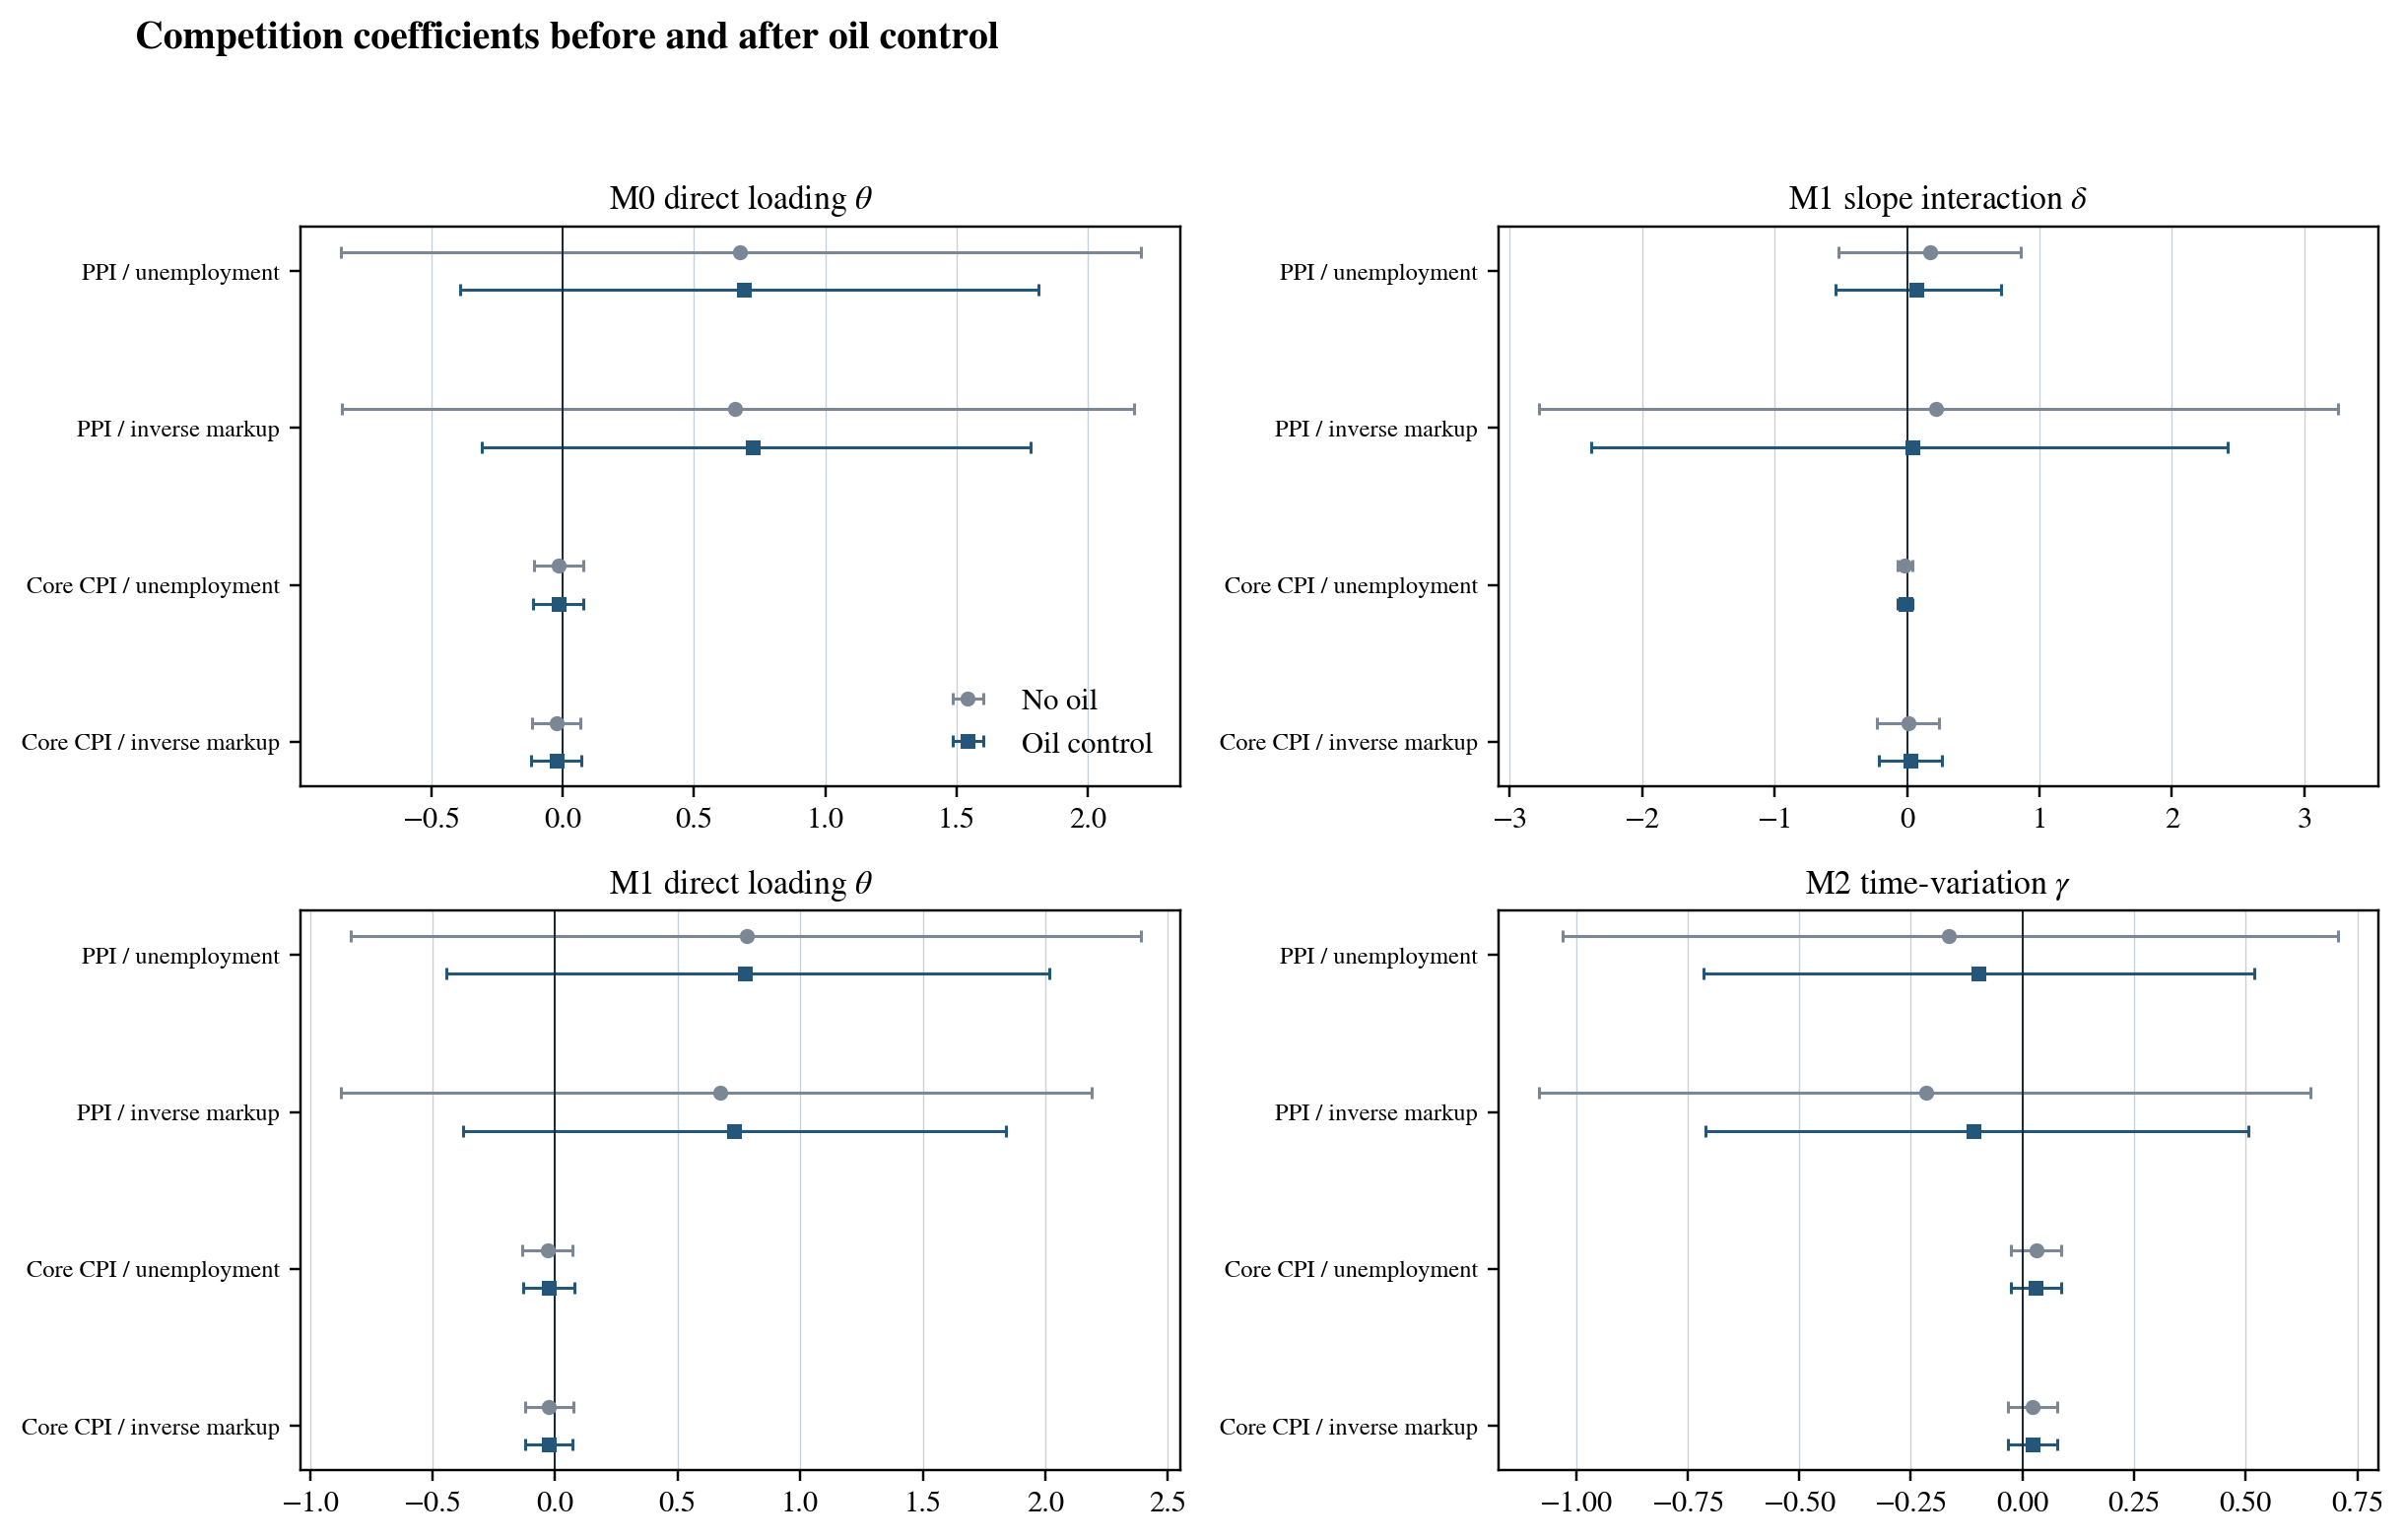
\includegraphics[width=0.91\linewidth]{oil_parameter_comparison.png}
\caption{Competition coefficients before and after the fixed oil-control extension.}
\end{figure}

M2 does not reveal time variation after oil is included:
\[
\theta_0=0.731[-0.374,1.853],\qquad
\gamma=-0.098[-0.714,0.518].
\]
M3 remains weak, and M4 still gives
$\lambda=0.425[-4.024,5.513]$ with zero-crossing derived slope coefficients. The oil
control improves the inflation residual equation but cannot solve the multiplicative
identification of $\lambda\theta_0$ and $\lambda\gamma$.

Core CPI is a useful placebo-like comparison. Its M0 loading changes only from
$-0.016[-0.111,0.078]$ to $-0.015[-0.115,0.078]$. Its M2 $\gamma$ remains directionally
positive but zero-crossing. The same oil terms therefore do not manufacture a common HSA
sign across price indices.

% -----------------------------------------------------------------------------
\section{Oil-Control Prediction, Recovery, and Convergence}

\begin{figure}[H]
\centering
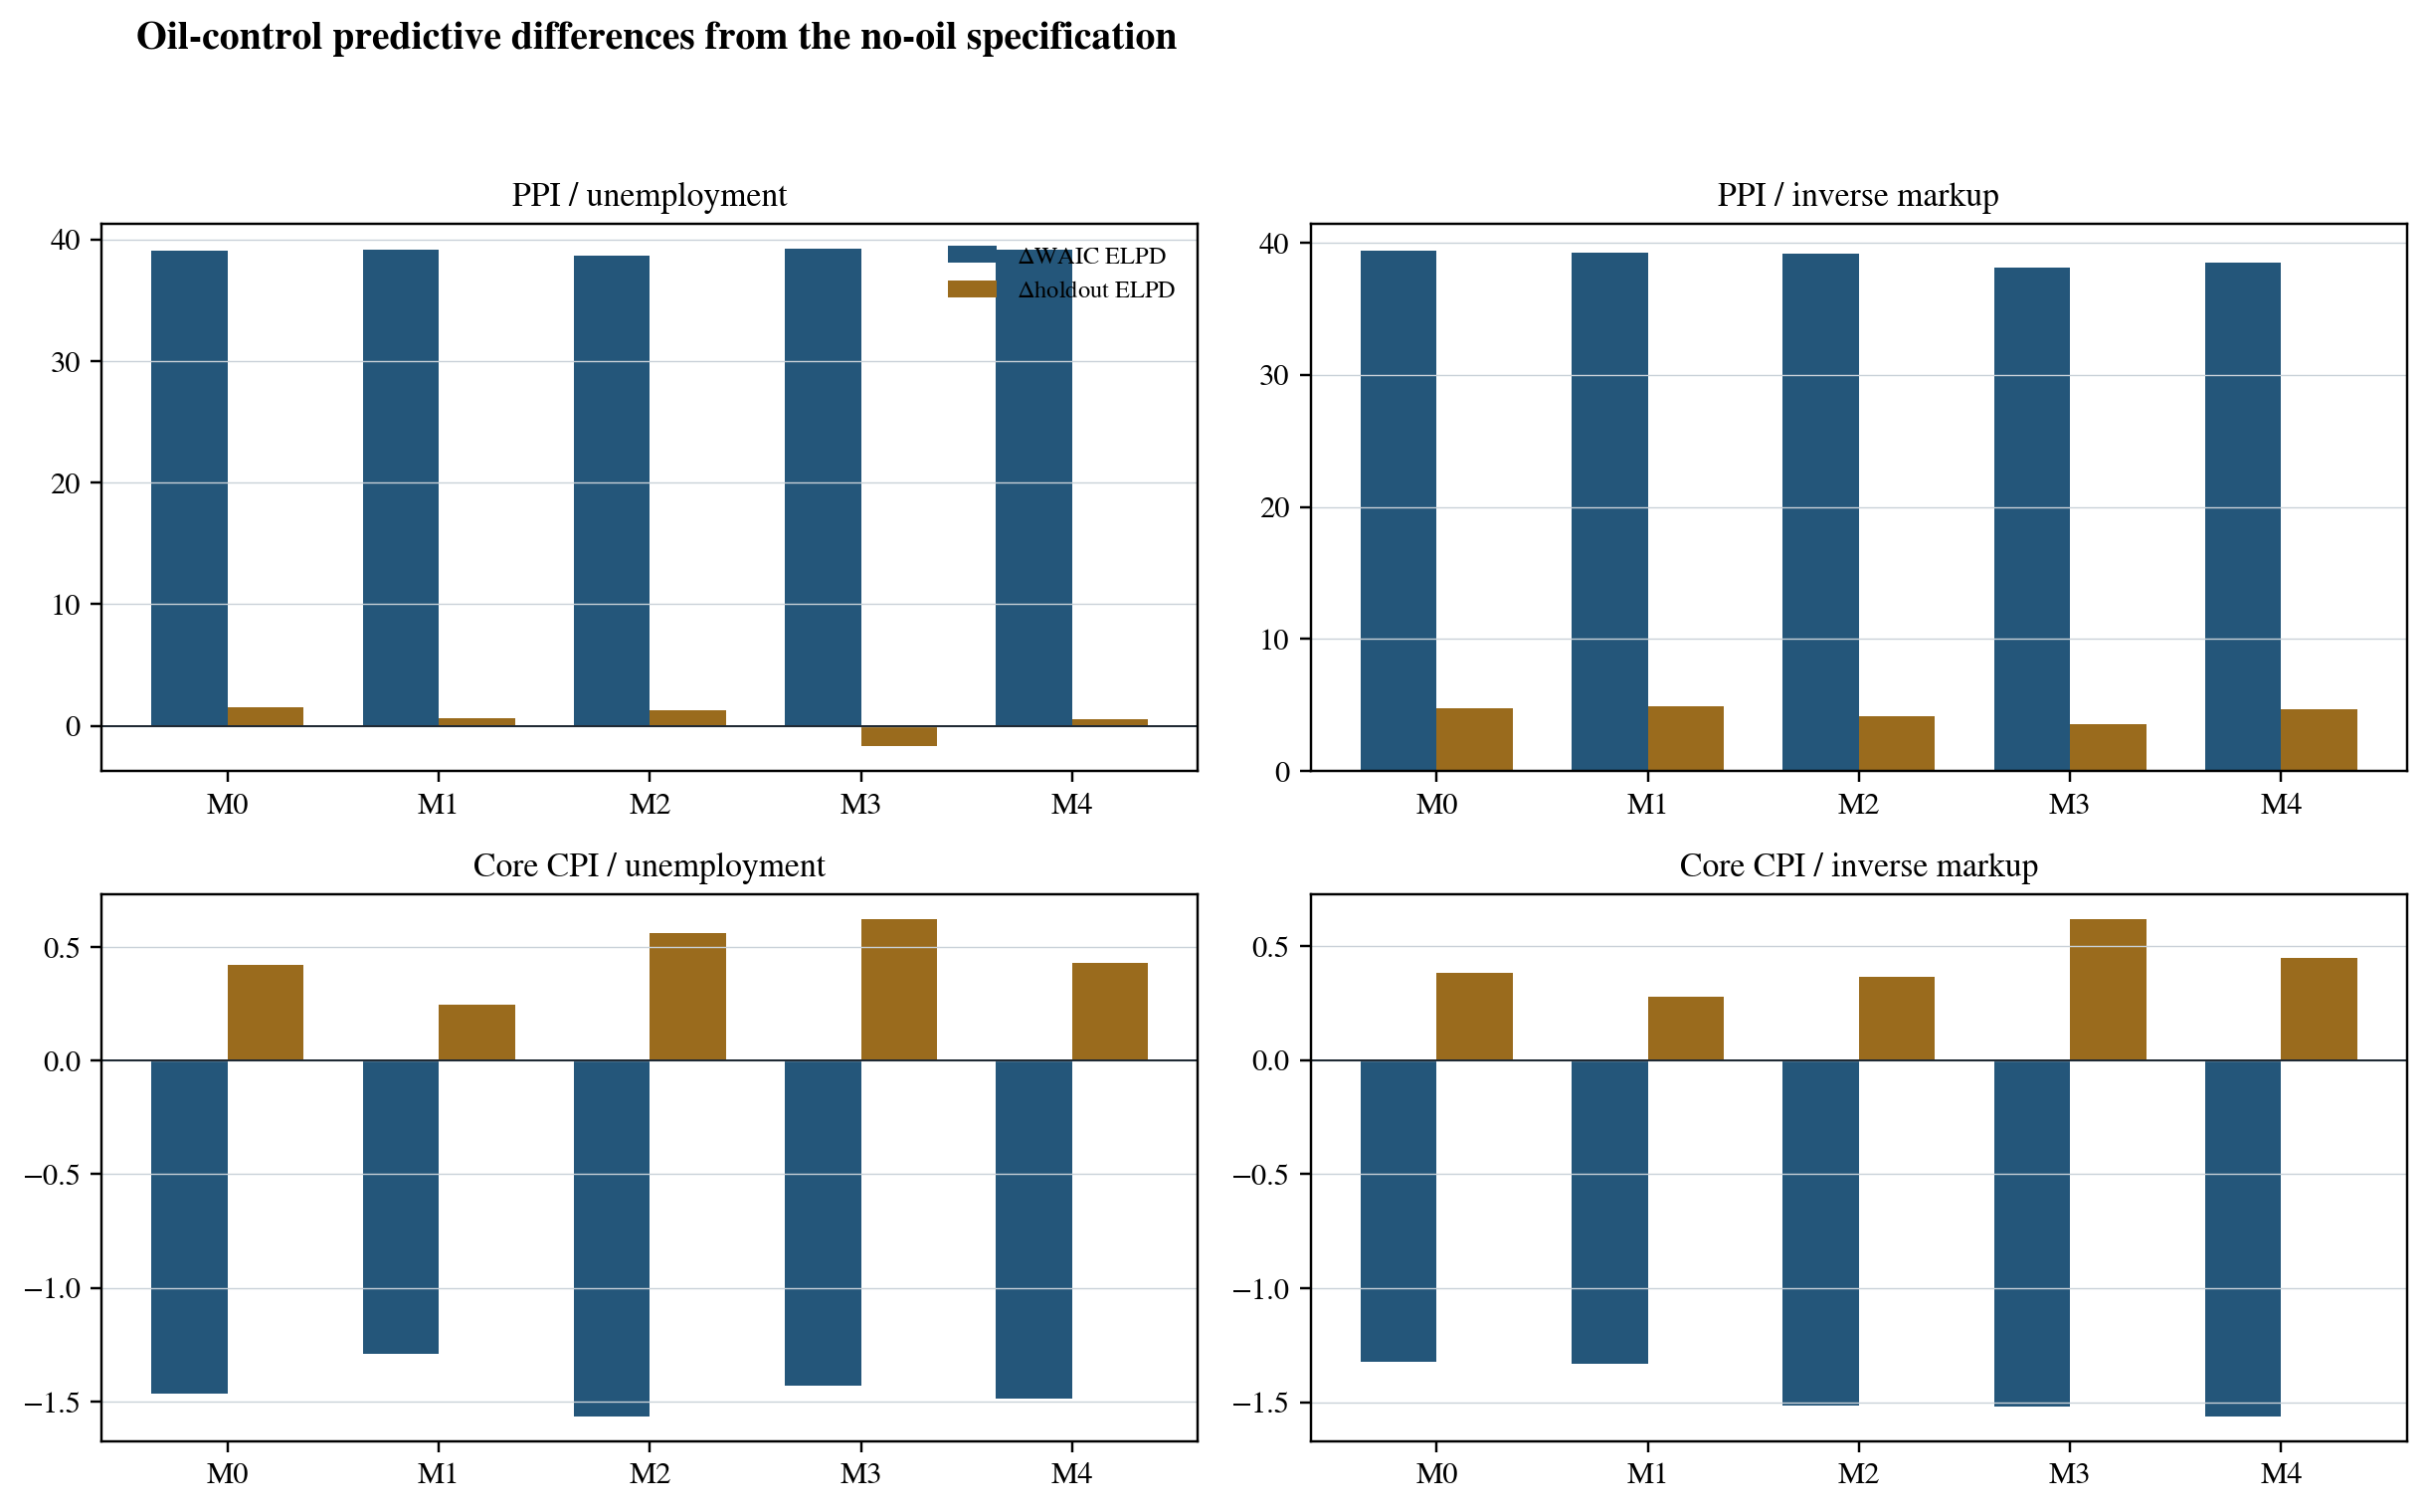
\includegraphics[width=0.91\linewidth]{oil_prediction.png}
\caption{Oil-control predictive differences relative to each otherwise identical no-oil model.}
\end{figure}

PPI WAIC improves by roughly 38--39 ELPD units across M0--M4. Its PSIS-LOO comparisons
point in the same direction, but maximum Pareto $k$ remains above one, so the LOO magnitudes
are not used as decisive evidence. Holdout behavior is more informative and less uniform.
With inverse markup, oil raises holdout ELPD by 3.53--4.91 and lowers RMSE by 0.58--1.01.
With the unemployment gap, M0 raises holdout ELPD by 1.55 but raises RMSE by 0.21, while M3
deteriorates materially. Oil is clearly useful for fitting PPI, but its out-of-sample benefit
depends on the activity proxy and model complexity.

For Core CPI, WAIC falls by 1.3--1.6. Holdout ELPD rises by only 0.25--0.62 and RMSE changes
by less than 0.015. These small, mixed changes do not justify describing oil as an important
Core-CPI control in this sample.

\begin{table}[H]
\centering
\caption{Oil versus no-oil predictive comparison; firm-weighted cells}
\scriptsize
\resizebox{0.91\linewidth}{!}{\begin{tabular}{@{}llrrrr@{}}
\toprule
Cell & Model & $\Delta$WAIC & $\Delta$holdout & $\Delta$RMSE & max $k$ \\
\midrule
PPI / unemployment & Constant theta & 39.077 & 1.555 & 0.213 & 1.20 \\
PPI / unemployment & Free static combined & 39.169 & 0.620 & 0.747 & 1.21 \\
PPI / unemployment & Varying theta & 38.648 & 1.254 & 0.334 & 1.28 \\
PPI / unemployment & Free dynamic & 39.213 & -1.692 & 2.083 & 1.19 \\
PPI / unemployment & HSA-restricted dynamic & 39.201 & 0.565 & 1.076 & 1.25 \\
PPI / inverse markup & Constant theta & 39.420 & 4.802 & -0.951 & 1.40 \\
PPI / inverse markup & Free static combined & 39.237 & 4.914 & -1.008 & 1.28 \\
PPI / inverse markup & Varying theta & 39.178 & 4.152 & -0.803 & 1.11 \\
PPI / inverse markup & Free dynamic & 38.088 & 3.534 & -0.577 & 1.17 \\
PPI / inverse markup & HSA-restricted dynamic & 38.495 & 4.682 & -0.814 & 1.50 \\
Core CPI / unemployment & Constant theta & -1.466 & 0.423 & -0.004 & 0.61 \\
Core CPI / unemployment & Free static combined & -1.290 & 0.246 & -0.000 & 0.64 \\
Core CPI / unemployment & Varying theta & -1.566 & 0.561 & -0.009 & 0.61 \\
Core CPI / unemployment & Free dynamic & -1.429 & 0.623 & -0.009 & 0.61 \\
Core CPI / unemployment & HSA-restricted dynamic & -1.487 & 0.428 & -0.003 & 0.62 \\
Core CPI / inverse markup & Constant theta & -1.324 & 0.380 & -0.003 & 0.53 \\
Core CPI / inverse markup & Free static combined & -1.331 & 0.277 & -0.002 & 0.56 \\
Core CPI / inverse markup & Varying theta & -1.514 & 0.363 & -0.007 & 0.49 \\
Core CPI / inverse markup & Free dynamic & -1.520 & 0.618 & -0.015 & 0.63 \\
Core CPI / inverse markup & HSA-restricted dynamic & -1.562 & 0.449 & -0.006 & 0.66 \\
\bottomrule
\end{tabular}
}
\end{table}

Recovery was rerun with the fitted oil contribution retained in the data-generating process.
At the observed standardized static effects $(s_\delta,s_\theta)=(0.06,0.11)$, propagated-
state suggestive recovery is 0.05 for $\delta$ and 0.40 for PPI $\theta$. Core-CPI rates are
0.05 and 0.55. At $s_\gamma=0.10$, suggestive recovery is 0.60 for PPI and 0.35 for Core CPI.

\begin{table}[H]
\centering
\caption{Oil-control propagated-state recovery at observed-scale effects}
\begin{tabular}{@{}llrrrr@{}}
\toprule
Outcome & Parameter & True effect & Suggestive & Strong & Coverage \\
\midrule
PPI & $\delta$ & 0.06 & 0.05 & 0.00 & 1.00 \\
PPI & $\theta$ & 0.11 & 0.40 & 0.00 & 1.00 \\
PPI & $\gamma$ & 0.10 & 0.60 & 0.00 & 1.00 \\
Core CPI & $\delta$ & 0.06 & 0.05 & 0.00 & 1.00 \\
Core CPI & $\theta$ & 0.11 & 0.55 & 0.05 & 1.00 \\
Core CPI & $\gamma$ & 0.10 & 0.35 & 0.05 & 1.00 \\
\bottomrule
\end{tabular}

\end{table}

These rates remain below a conventional power target. The realized PPI sample becomes more
directional after oil control, but repeated-sample recovery still warns against treating
that posterior as reliable structural sign identification.

\begin{table}[H]
\centering
\caption{Oil-control convergence; firm-weighted unemployment-gap cells}
\begin{tabular}{@{}llrr@{}}
\toprule
Outcome & Model & Max R-hat & Min bulk ESS \\
\midrule
PPI & Constant theta & 1.0031 & 2523.0 \\
PPI & Free static combined & 1.0008 & 2625.8 \\
PPI & Varying theta & 1.0013 & 6481.0 \\
PPI & Free dynamic & 1.0005 & 5795.2 \\
PPI & HSA-restricted dynamic & 1.0008 & 3901.3 \\
Core CPI & Constant theta & 1.0021 & 2595.4 \\
Core CPI & Free static combined & 1.0020 & 2415.0 \\
Core CPI & Varying theta & 1.0004 & 6493.4 \\
Core CPI & Free dynamic & 1.0005 & 6488.4 \\
Core CPI & HSA-restricted dynamic & 1.0032 & 1755.0 \\
\bottomrule
\end{tabular}

\end{table}

All 90 observed fits pass: maximum R-hat is 1.0046 and minimum bulk ESS is 1,106.3. Across
the 560 recovery fits, maximum R-hat is 1.0180 and minimum bulk ESS is 344.4. Persistent
AR(1) errors leave the PPI M0 result essentially unchanged:
$\theta=0.690[-0.501,1.916]$ and
$\beta_{o,0}=0.112[0.089,0.134]$. The substantive limits are identification and predictive
stability, not MCMC convergence.

% -----------------------------------------------------------------------------
\section{Why the Dynamic HSA Exercise Does Not Succeed}

The evidence points to several complementary explanations rather than one coding or sampling
defect.

\begin{enumerate}
\item \textbf{Low signal-to-noise ratio.} QoQ PPI inflation has an SD of 8.59 annualized
percentage points. Core CPI is smoother, but its estimated competition contributions are
also small. In both outcomes the observed standardized direct and slope effects remain below
the reliable recovery region.

\item \textbf{Short aggregate sample.} The NKPC has only 83 quarters. Dynamic models add
several competition interactions while estimating inflation persistence, the forward term,
the activity slope, and innovation variance. Aggregate time-series variation is limited.

\item \textbf{The forward coefficient is weakly learned.} $\alpha_f$ retains nearly its prior
dispersion. Expectation and persistence uncertainty consumes variation that might otherwise
identify small competition contributions.

\item \textbf{State uncertainty is real but not decisive.} Capital IQ measurement error is
material. Yet oracle-state recovery remains weak at observed effects, showing that a perfectly
known cycle would not by itself solve the problem.

\item \textbf{Empirical coordinate versus theoretical $N$.} Capital IQ inverse concentration
is not literally the HSA active-firm stock. The negative firm-weighted slow loading and the
near-zero revenue-weighted loading reveal an unstable level mapping. A weak structural result
may reflect measurement mapping as well as lack of an economic mechanism.

\item \textbf{Multiplicative HSA weak identification.} The restricted likelihood depends on
$\lambda\theta_0$ and $\lambda\gamma$. Near zero, $\lambda$ is weakly identified and sign
symmetries remain. A broad $N(0,10^2)$ prior correctly exposes this rather than imposing a
preferred sign or fixed value.

\item \textbf{The sign pattern is not stable across price indices.} PPI average direct
loadings lean positive and PPI $\gamma$ leans negative. Core CPI produces the reverse pattern.
Because neither set excludes zero, pooling or selecting one outcome would not establish a
common HSA sign.

\item \textbf{No catastrophic linear collinearity to fix.} Condition numbers are modest.
Dropping one regressor solely to manufacture significance would not address the underlying
signal limitation and would change the economic question.

\item \textbf{Activity and expectation proxies are imperfect.} GDP-deflator expectations
are not PPI-specific, and headline-CPI expectations are not Core-CPI-specific. The aggregate
inverse markup is a proxy for theoretical real marginal cost, while the unemployment gap is
generated using an estimated natural rate. The present conditional regression does not
instrument these variables.

\item \textbf{Dynamic models do not predict better consistently.} All twelve PPI dynamic
holdout ELPD differences are negative. In Core CPI, tiny improvements for M1 or isolated M2
cells coexist with clear M3/M4 losses. The extra flexibility does not earn stable out-of-sample
support.

\item \textbf{Oil control clarifies but does not complete identification.} The fixed oil
terms explain a large share of QoQ PPI variation and narrow the PPI direct-loading posterior.
They do not make its 95\% interval exclude zero, raise observed-scale recovery to a reliable
level, identify $\delta$ or $\gamma$, or resolve the multiplicative HSA restriction.
\end{enumerate}

These points rule out a convenient rescue by longer MCMC alone. Longer chains reduce Monte
Carlo error, but they do not increase economic variation or repair an uncertain measurement
mapping.

% -----------------------------------------------------------------------------
\section{Interpretation, Scope, and Next Empirical Steps}

\subsection{What may be carried forward}

The QoQ switch is useful. It aligns horizons, removes mechanical YoY overlap, and produces
direct coefficients that are visibly updated from symmetric zero-mean priors. The PPI
direction is positive and the Core-CPI direction is negative; both survive adding a slow
slope and the AR(1) error law. The robust statement is therefore about outcome-specific
empirical updating, not a common structural sign.

\subsection{What may not be claimed}

The 95\% intervals do not identify the theoretical sign for either outcome. $\gamma$,
$\lambda$, and both HSA derived slope terms are not identified. There is no valid current
claim that HSA dynamic beats CES in marginal likelihood, nor that $\lambda$ is a demand
elasticity. The time-varying median paths cannot be interpreted as identified historical
evolution.

\subsection{Admissible next steps}

\begin{enumerate}
\item Move from aggregate $T=83$ to industry-by-quarter variation while maintaining an
inflation-cut competition measurement block. This is the most direct way to raise information
without tuning priors to the desired sign.
\item Validate the mapping from Capital IQ inverse concentration to an active-firm stock using
external firm-stock or entry/exit data. The mapping should be tested before assigning a
structural interpretation to $\lambda$.
\item Use PPI-specific and Core-CPI-specific expectation measures if defensible historical
series become available, and propagate expectation uncertainty rather than treating either
proxy as exact.
\item Address activity endogeneity with an economically defensible instrument or explicit shock
system. A more elaborate state law should not substitute for identification of $x_t$.
\item If a larger panel or longer comparable sample becomes available, rerun simulation recovery
before the empirical HSA restriction. The minimum detectable $\theta$, $\gamma$, and slope
effects should remain predeclared.
\end{enumerate}

The appropriate current specification for reporting remains constant theta separately by
price index, described as outcome-specific directional evidence. For PPI, the prespecified
current-plus-lagged oil control is the better residual specification; for Core CPI it is a
reported robustness exercise rather than a necessary control. Free and restricted dynamic
models remain diagnostics of what the aggregate data cannot yet distinguish.

% -----------------------------------------------------------------------------
\section{Reproducibility and Audit Trail}

The report uses only saved results from
\code{tests/gustavo\_state\_capitaliq\_cycle}. The competition measurement draws are paired
and reused byte-for-byte across the inflation models. The staged and dynamic manifests record
the same processed-data SHA-256 hash and the same two measurement-draw hashes.

The dynamic run contains 27 observed fits: 24 IID fits from two Capital IQ cycles, two
activity measures, three dynamic models, and full/train samples, plus three full-sample AR(1)
robustness fits. It also contains 300 varying-theta recovery fits. The preceding staged run
contains 17 observed fits and 640 free-static recovery fits.

The Core-CPI extension contains 45 observed fits: 40 IID full/train fits from two cycles,
two activities, and all five M0--M4 models, plus five full-sample AR(1) robustness fits. It
also contains 480 free-static and 300 varying-theta recovery fits. The saved Core-CPI manifest
records maximum observed R-hat 1.0036 and minimum bulk ESS 1,220.2. A separate 45-fit smoke
run verified plumbing before the full run; its short-chain posterior is not used in this report.

The oil extension contains 90 observed fits: 80 IID full/train fits from two outcomes, two
cycles, two activities, and all five M0--M4 models, plus ten full-sample AR(1) robustness
fits. It also contains 560 recovery fits. The saved manifest records maximum observed R-hat
1.0046 and minimum bulk ESS 1,106.3; recovery maximum R-hat is 1.0180 and minimum bulk ESS
344.4. The state-draw hashes are unchanged from the no-oil runs.

Assets and tables are regenerated with:
\begin{verbatim}
PYTHONPATH=src:. python docs/report/qoq_gustavo_capitaliq/build_assets.py
\end{verbatim}
The Core-CPI estimation is reproduced with:
\begin{verbatim}
PYTHONPATH=src:. python \
  tests/gustavo_state_capitaliq_cycle/run_core_cpi_validation.py \
  --mode full --workers 4
\end{verbatim}
The oil-control estimation is reproduced with:
\begin{verbatim}
PYTHONPATH=src:. python \
  tests/gustavo_state_capitaliq_cycle/run_oil_control_validation.py \
  --mode full --workers 4
\end{verbatim}
The LaTeX report is compiled from this directory with:
\begin{verbatim}
latexmk -pdf qoq_hsa_report.tex
\end{verbatim}

The detailed numerical records remain in \code{RESULTS\_STAGED.md},
\code{RESULTS\_DYNAMIC.md}, \code{RESULTS\_CORE\_CPI.md}, and
\code{RESULTS\_OIL\_CONTROL.md}; the frozen equations and
interpretation rules remain in \code{SPECIFICATION.md}. Structural claims remain gated by
identification and recovery rather than computational convergence alone.

\end{document}
